\chapter{نتایج و تفسیر آنها}
\clearpage
\section{مقدمه}
کشف گرافن با پراکندگی خطی آن باعث شد که الکترون‌ها مانند فرمیون های بدون جرم دیراک حرکت کنند [1،2]. وجود نقاط دیراک در گرافن باعث ایجاد خواص الکترونیکی، مکانیکی و نوری متفاوتی نسبت به سایر آلوتروپ های کربن می شود [3]. شناسایی این رفتارهای جدید رویای وسایل الکترونیکی را بسیار دست یافتنی تر به نظر می رساند. از سوی دیگر، فقدان شکاف نوار و تحرک بالای حامل ها، کاربرد گرافن را در دستگاه های نیمه هادی محدود می کند. بنابراین، مواد دو بعدی دیگر مانند سیلیس [4]، ژرمانن [5]، استانن [6]، فسفر سیاه [7] و آنتیمونن [8]، دی سولفید مولیبدن [9]، دیکالکوژنیدهای فلزی میانی (\ce{TMDC}) [10] و نیترید بور شش ضلعی (\ce{h-BN}) [11] به آسانی با روش های سنتز قوی در دسترس هستند و با موفقیت در کاربردهای الکترونیکی استفاده شده اند [12-14]. اخیراً، ماده دو بعدی دیگری به نام بوروفن بر روی بستر نقره [15،16] شرایط خلاء بسیار بالا بر اساس محاسبات نظری [17-19] سنتز شده است که به دلیل خواص خارقالعاده‌اش جلب توجه میکند. خواص مکانیکی جذاب آن را به رقیبی برای گرافن تبدیل کرده است [15]. همچنین دارای خواص فلز ناهمسانگرد است که منجر به خواص فیزیکی وابسته به جهت مناسب برای استفاده در دستگاه های انعطاف پذیر می شود.

با گذشت زمان، قانون مور برای موثر ماندن با چالش های جدی تری مواجه خواهد شد. با توجه به اینکه الکترونیک سنتی تنها بر اساس حمل و نقل و ذخیره بار الکتریکی استوار است، ادامه فرآیند کوچک سازی محدودیت های بیشتر و چالش های عمیق تری را به همراه خواهد داشت. بنابراین، دستگاه های مبتنی بر اصول جدید تبدیل به یک کانون در دوران پس از مور 1،2 شده اند. اسپینترونیک\LTRfootnote{Spintronics} یکی از فناوری هایی است که ممکن است قانون مور را به چالش بکشد. هدف اسپینترونیک درک برهمکنش اسپین ذرات با محیط جامد اطراف آنها، به ویژه تأثیر اسپین الکترون بر رسانایی (یا جریان) است. مشکل اصلی در اسپینترونیک ساخت دستگاه های مبتنی بر اسپینترونیک است. از زمان کشف GMR در سال 1988 3،4، اسپینترونیک شامل ترابرد گشتاور اسپینی 5،6، اسپینترونیک نیمه هادی، اسپینترونیک تک الکترونی و غیره، به عنوان یک زمینه تحقیقاتی جدید فعال بوده است. یکی از شگفت انگیزترین کاربردهای اسپینترونیک اثر شیر اسپینی\LTRfootnote{Spin Valve} 5 است که بادستکاری زاویه نسبی مغناطش زیرلایه مغناطیسی در لیدها فابل تنظیم است. شیر اسپینی اولین بار در سال 1991 توسعه یافت، که بعداً صنعت حسگرهای مغناطیسی، هدهای دیسک سخت و حافظه‌های دسترسی تصادفی مغناطیسی (MRAM) 8-11 را متحول کرد. دستگاه شیر اسپینی از دو یا چند اتصال مغناطیسی تشکیل شده است. در یک دستگاه شیر اسپینی با دو اتصال مغناطیسی، بسته به اینکه اتصالات مغناطیسی در جهت جریان درون صفحه (CIP) یا عمود بر صفحه (CPP) باشد، دو ساختار هندسی متفاوت تشکیل می شود. مقاومت مغناطیسی به پدیده ای اطلاق می شود که مقاومت یک فلز یا نیمه هادی با یک میدان مغناطیسی خارجی تغییر می کند.
% تصویر برای cip و cpp

در میان آلوتروپ های مختلف پیشنهاد شده برای بوروفن [20-23]، $\beta_{12}$  پایدارترین تک لایه بور [24].همچنین نسبت به سایر آلوتروپ های خود در برابر اکسیداسیون بی اثرتر است، که مزیت خوبی برای کاربرد دستگاه ها در آینده است [16].


\subsection{شبکه شش گوشی پنهان}
بوروفن $\beta_{12}$ یک ورقه گرافن مانند دوبعدی پایدار است که توسط محاسبات و آزمایشات اصول اولیه\LTRfootnote{First Principle Calculations} تأیید شده است [26]. ساختار $\beta_{12}$ یک شبکه مستطیلی با تقارن \lr{P2MM} است با پایه ای که دارای پنج اتم است که در شکل \ref{fig:borophene}(e) نشان داده شده است. ثابت های شبکه مستطیلی \lr{\AA}2.92 و \lr{\AA}5.06 هستند. [53]، بنابراین فاصله اتمی \ce{B-B} طبق محاسبات اصول \lr{\AA} $l=1.69$ است. اولیه\LTRfootnote{First Principle Calculations}، ثابت شبکه \lr{BNR} های بدون اتم مرکزی (بوروفن با ساختار لانه زنبوری) 0.4\% کمتر از بوروفن $\beta_{12}$ است، و چگالی بار در اطراف اتم مرکزی، در مقایسه با سطح هم سطح لانه زنبوری چگالی بار، رقیق شده است. از سوی دیگر، شش پیوند درون صفحه در $\beta_{12}$ ($\sigma$ پیوندهای) دارای تقارن انتقالی هستند. بنابراین ما شبکه ای از لانه زنبوری داریم که در $\beta_{12}$ پنهان شده است، که در آن اتم مرکزی به عنوان یک الکترون دهنده عمل می کند تا پیوندهای $\sigma$ داخل ساختار لانه زنبوری را پر کند [54]. 

اگرچه ساختار $\beta_{12}$، بر خلاف گرافن و سیلیسین، به جای ساختار شبکه شش ضلعی، دارای ساختار شبکه ای مستطیلی است، محاسبات اصول اولیه نشان داد که چگالی الکترونی موضعی حالات \lr{(LDOS)} در $\beta_{12}$ در مرکز سلول واحد آن است. بسیار کمتر از همسایگان خود [25]، و بنابراین می توان انتظار داشت که بوروفن نیز میزبان مخروط های دیراک باشد. فرمیون های دیراک توسط آزمایش های طیف سنجی انتشار نوری با وضوح زاویه ای \lr{(ARPES)} و محاسبات اصل اول مشاهده می شوند [26]. ساختار نوار به خوبی توسط یک مدل اتصال محکم بازتولید شده است، به طوری که، به دلیل ساختار مسطح کامل آن، در نظر گرفتن تنها اوربیتال های $P_z$ کافی است. اگرچه بوروفن بر روی بسترهای فلزی سنتز شده است، اما هنوز جدا نشده است، و بسیاری از درک خواص نوری الکترونیکی آن از تئوری و محاسبات ناشی می شود. به طور خاص، مطالعات تئوری تابعی چگالی \lr{(DFT)} ساختار نواری آلوتروپ های مختلف بوروفن را بررسی کرده است. این مطالعات پیش‌بینی می‌کنند که ساختارهای کریستالی کم انرژی مختلف میتوانند منجر به رفتار فلزی یا نیمه فلزی شوند [25،27-30]، ممکن است حاوی مخروطهای دیراک در یا نزدیک انرژی فرمی [30-35] باشند و اغلب ناهمسانگردی رسانایی درون صفحه را نشان میدهند. به پیکربندی اتصال ناهمسانگرد [36،37]. همچنین نشان داده شده است که علاوه بر فرمیونهای دیراک، مدلهای دیراک در نقاط تماس سه نواری نیز وجود دارد و شکل صریح همیلتون‌های مؤثر آنها به دست میآید [38]. مطالعات نظری زیادی روی $\beta_{12}$ انجام شده است، [39-41] از جمله پیشبینی رفتار ابررسانا در محدوده دمایی 10-20 کلوین به دلیل جرم اتمی کوچک آن، که باعث جفت شدن قوی الکترون-فونون میشود [42].
همچنین نشان داده شده است که نانوروبانهای دارای لبه‌های آرمچیر بدون بار لبه‌ای هستند، زیرا اتمهای لبه آنها به یک زیرشبکه ختم میشوند. \lr{LDOS} در نزدیکی انرژی فرمی، چگالی الکترونی فضایی حالتها در کل محل نانوروبان بوروفن ارمچیر با یک مکان خالی در لبه بالایی خالی، یک جای خالی، و دو جای خالی در وسط نانو نوار رسم شده است. نوع بنابراین، اگرچه آنها به طور کلی نیمه هادی هستند، اما حالت های صفر را می توان در عرض های به درستی انتخاب شده ایجاد کرد [58]. این باعث می شود که نانوروبان های لبه ارمچیر بین رفتارهای نیمه هادی و هادی در نوسان باشند. بنابراین، رفتار مشابه مشاهده شده در \lr{BNR} ها را می توان به عنوان تاییدی بر وجود شبکه لانه زنبوری پنهان در نظر گرفت.

توابع موج به دست آمده از سایت های a،b،d و e به دو زیرشبکه تقسیم می شوند. ما زیرشبکه A را به اتم های a,d و زیرشبکه B را به اتم های b,e نامیدیم. نشان داده شده است که یک مدل اتصال محکم پنج نوار با انتخاب ضرایب انرژی در محل و پرش مناسب به خوبی با\gls{محاسبات اصول اولیه} مطابقت دارد [26،55]. در این مدل، انرژی های موجود در محل، تقارن وارونگی سازه را به دلیل تأثیرات زیرلایه \lr{Ag} می شکنند و به همین دلیل به آن مدل نا متقارن وارونگی \lr{(INS)} می گویند. به منظور حذف اثرات زیرلایه، یک مدل متقارن وارونگی \lr{(IS)} تعریف شده و برای افزودن همگنی، یک مدل همگن معرفی شده است [38]. ما همه این ضرایب را در جدول \ref{tbl:hoppingtable} فهرست کردهایم. همیلتونین پیوندی محکم از بوروفن $\beta_{12}$ که صرفاً اوربیتالهای $P_z$ را در فضای واقعی در نظر میگیرد، میتواند به صورت زیر ارائه شود:
\begin{equation}
  \mathcal{H}=\sum_{i}\varepsilon_i a_i^\dagger a_i +\sum_{ij} t_{ij}a_i^\dagger a_j+c.c
\end{equation}
که $a_i^\dagger$($a_i$) عملگرهای خلق و (فنا) هستند که بر الکترون‌های $\pi$ در مکان $i$ام عمل میکنند، $\varepsilon_i$ انرژی مکان $i$ام و $t_{ij}$ انرژی جهش بین نزدیک ترین همسایه اول است.
درصورتی که بخواهیم ملاحضات اسپینی را لحاظ کنیم:
\begin{equation}
  H= H_L + H_R + H_c + H_T,
\end{equation}
که:
\begin{equation}
H_{L}=\sum\limits_{i\in L,\sigma }{\left( E_{L}+\sigma M_{L} \right)} a_{i\sigma }^{\dagger} a_{i\sigma }-\sum\limits_{i,i+\alpha \in L,\sigma}{\left( t_{\alpha } a_{i\sigma}^{\dagger} a_{i+\alpha \ \sigma }+H.c.\right)},
\end{equation}
\begin{equation}
\begin{split}
H_{R}=\sum_{i\in R,\sigma}{\left( E_{R}+\sigma M_{R} cos\phi M_{R}\sin \phi\right)} a_{i\sigma}^{\dagger} a_{i\sigma } \\
-\sum_{i\in R,\sigma} t_{\alpha } a_{i\sigma}^{\dagger} a_{i+\alpha\sigma}+H.c.,
\end{split}
\end{equation}
\begin{equation}
H_{C}=\sum_{i\in \ C,\sigma }{{{E}_{C}}}a_{i\sigma }^{\dagger}{{a}_{i\sigma }}-\sum_{i,i+\alpha \in \ C,\sigma }{({{t}_{\alpha }}\ a_{i}^{\dagger }{{a}_{i+\alpha }}+H.c.)},
\end{equation}
\begin{equation}
H_{T}=-\sum_{i\in \ C,i+\alpha \in L,R,\sigma}{{{t}_{\alpha }}}\ a_{i\sigma }^{\dagger }{{a}_{i+\alpha \ \sigma }}+H.c.,
\end{equation}
جایی که $E_L$، $E_R$ و $E_C$ انرژی‌های جایگزیده در نانونوارهای بوروفن در سمت چپ و راست و منطقه مرکزی هستند که می‌توانند توسط ولتاژ گیت تنظیم شوند، بسته به مکان نقطه توری، همانطور که در جدول \ref{tbl:hoppingtable} نشان داده شده است. $a^{\dagger}_{i\sigma}$ ($a_{i\sigma}$) اپراتورهای ایجاد (انحلال) الکترون در سایت $i$ با شاخص اسپین ($\sigma$) هستند. $M_L$ و $M_R$ مغناطیس‌گرایی الکترودهای FM چپ و راست هستند و $\theta$ زاویه بین جهت‌دهی‌های $M_L$ و $M_R$ است. جریان الکتریکی که از طریق سیستم جاری می‌شود ممکن است با استفاده از روش تابع سبز غیرتعادل مشخص شود.

\begin{table}
  \centering
  \caption{پارامترهای پرش \lr{$\beta_{12}$-borophene} معرفی شده توسط \lr{Ezawa}\cite{ezawaTripletFermionsDirac2017}\label{tbl:hoppingtable}}
\begin{latin}
  \begin{tabular}{cccccccc}
  \toprule
   & H & INS & IS &
   & H & INS & IS\\
  \midrule
  $\varepsilon_a$& 0 &  0.196 &  0.196 & $t_{ab}=t_{de}$& -2 & -2.04 & -2.04 \\
  $\varepsilon_b$& 0 & -0.058 & -0.058 & $t_{ac}=t_{ce}$& -2 & -1.79 & -1.79 \\
  $\varepsilon_c$& 0 & -0.845 & -0.845 & $t_{ae}$& -2 & -2.12 & -2.12   \\
  $\varepsilon_d$& 0 &  0.196 & -0.058 & $t_{bc}=t_{cd}$& -2 & -1.84 & -1.84 \\
  $\varepsilon_e$& 0 & -0.058 &  0.196 & $t_{bd}$& -2 & -1.91 & -1.91  \\
  \bottomrule
  \end{tabular}
  \end{latin}
\end{table}
\section{رسانش کلید ساخت وسایل الکترونیکی}
در اینجا باید اشاره کنیم که در میان تمام خاصیت هایی که مواد دوبعدی دارند رسانندگی اهمیت ویژه ای برای ساخت ریز دستگاه های اکترونیکی دارند. بنابراین رسانش را در سه حالت کلی بررسی میکنیم
۱. رسانش کوانتومی بار
۲. رسانش کوانتومی اسپین
۳. رسانش کوانتومی درهها
\section{رسانش کوانتومی بار}
طیف های ترابرد نانوروبان های بوروفن بکر \lr{(BNRs)} ساختار پله ای شناخته شده ای را نشان می دهد. ارتفاع پله‌ها مربوط به تعداد نوارهای انرژی است که از انرژی داده شده عبور می کنند. علاوه بر این، برخلاف نانوروبانهای گرافن \lr{(GNRs)}، تعداد کانالهای رسانایی در انرژی فرمی ثابت نمی‌ماند [57] و با افزایش عرض نانوروبانها افزایش می‌یابد که در نانوروبانهایی با لبه زیگزاگ در مقایسه با لبهاارمچیر یک بیشتر دیده میشود [38]. دلیل وابستگی عرض به تعداد کانال های رسانایی در انرژی فرمی را می توان به وجود اتم مرکزی در داخل سلول واحد نسبت داد. هر یک از اتم های پایه در سلول واحد نوارهای $\beta_{12}$ می تواند روی لبه باشد و بر اساس اتم لبه، پنج نوع ابرسلول زیگزاگ در نظر گرفته می شود. وقتی اتم \lr{e} روی لبه قرار می گیرد، دیگر لبه زیگزاگی نخواهد بود، بنابراین در مجموع 16 نوع ابرسلول زیگزاگ دیده می شود. میتوانیم ابرسلول‌ها را با نام اتمهای لبه‌های بالا و پایین نامگذاری کنیم، مثلاً \lr{ZNBR-cd} که به اتم \lr{c} در لبه بالا و اتم d در لبه پایین ختم میشود. محاسبات ما نشان میدهد که اگرچه \lr{ZNBR-cd} با عرض\lr{\AA} 8.8 دارای شکافهای نوار بسیار کوچکی است، اما اغلب خواص فلزی را نشان میدهند. زیرا ابرسلول هایی که از هر دو انتها به یک سلول ختم می شوند در بسیاری از محاسبات استفاده شده اند [26،38]. در این تحقیق نیز همین ساختار مورد توجه قرار گرفته است. در مورد لبه های آرمچیر، هر لبه می تواند به \lr{b-d(ac-a)} ختم شود که آن را به ترتیب $\alpha$ ($\gamma$) می نامیم، بنابراین چهار نوع ابرسلول آرمچیر داریم که یک نمونه آن\lr{ABNR-$\alpha\alpha$}است.محاسبات ما نشان می دهد که برخلاف \lr{ZBNR} ها، نانوروبان های لبه آرمچیر دارای رفتار نیمه هادی یا فلزی وابسته به عرض روبان \lr{W} هستند، به طوری که برای عرض بیشتر از مقدار بحرانی \AA $W_c = 11.08$، رسانایی را می توان یافت و برعکس یا $W\leq W_c$، سیستم مانند یک نیمه هادی رفتار می کند. وابستگی حالت های الکترونی به عرض نانوروبان‌ها در یک شبکه لانه زنبوری با حل معادله دیراک (شرودینگر) با شرایط مرزی مناسب، که دارای توابع موج صفر در هر دو لبه نانوروبان هستند، درک می شود. بر اساس محاسبات انجام شده مشاهده می شود که نانوروبان هایی با لبه های زیگزاگی که لبه های بالایی و پایینی آنها به زیرشبکه های مختلف ختم می شود، توابع موج لبه ایجاد می کنند. همانطور که می دانیم، بر خلاف الکترون های بلوخ، حالت های لبه به طور تصاعدی در فواصل کوتاه از لبه‌ها تحلیل می روند. حالت های لبه در شکاف انرژی در نیمه هادی‌ها و همچنین در شکاف های جایگزیده در هادی‌ها قرار دارند.

%%%% این قسمت نیاز دارد که برخی از نمودارها که در مقالات نیاوردهایم بیاوریم و نتایج را حاصل محاسبات خود مطرح کنیم.

\section{رسانش کوانتومی بار نانونوارها در حضور انواع نقص}
وجود عیوب در مواد دو بعدی در حین ساخت آنها امری رایج است. به عنوان مثال، گرافن، با وجود پایداری حرارتی بالا، دارای عیوب گوناگونی در فرآیند رشد کریستال خود است [49،50]. از سوی دیگر، از آنجایی که پایداری حرارتی بوروفن کمتر از گرافن است، احتمال بروز نقص در هنگام ساخت بیشتر است [51]. بر خلاف سایر مواد دو بعدی، بوروفن اخیراً دارای فرآیندهای رشد لبه است و در حالی که شکل تعادل ترمودینامیکی آن تقریباً مستطیلی است، در مشاهدات تجربی مشاهده نشده است و در بیشتر موارد، ناهمواری‌های لبه وجود دارد [52]. در نتیجه، این فرض که اشکال‌ها لبه‌های متنوعی از ممکن است بر اساس عیوب نقطه لبه تشکیل شوند، بیش از یک فرض نظری ساده است. نقص‌ها می توانند به طور قابل توجهی بر خواص الکترونیکی مواد دو بعدی تأثیر بگذارند. به منظور بررسی نقش عیوب لبه در نانوروبان‌های بوروفن \lr{(BNRs)}، می‌توان با حذف یک یا دو اتم در لبه‌های \lr{BNR}، نقصهای منفرد ایجاد کرد. در این رساله رسانایی بوروفن $\beta_{12}$ را با روش \lr{NEGF} با کمک یک هامیلتونین \gls{تنگ بست} بدست می آوریم. نشان میدهیم که رسانایی به عرض نوارها و نوع لبه‌های نوار بستگی دارد. همچنین، از آنجایی که یک شبکه لانه زنبوری پنهان در داخل $\beta_{12}$ وجود دارد، نقصهای منفرد در لبه را می‌توان بر اساس یک مدل ساده توجیه کرد که در آن حالتهای لبه توسط حالت‌های ناشی از ناخالصی‌های لبه ضد تشدید ایجاد میشوند. در نهایت، ما اثرات اختلال‌های اندرسون را بررسی می‌کنیم و وابستگی آنها را به عرض نوار و قدرت پتانسیل اختلال نشان می‌دهیم.
\subsection{انواع عیوب}
در اینجا باید انواع عبوب را به نظر بیان کنیم و علت اهمیت آنها را بیان کنیم و بگوییم که چرا این عیوب را محاسبه کرده ایم.
\begin{itemize}
  \item جای خالی‌ها
  \item جایگزینی‌ها
  \item عیوب لبه‌ای
  \item عیوب میانی
  \item اختلال ضعیف
\end{itemize}
رسانایی نانوروبانهای $\beta_{12}$ \lr{(BNRs)} با نقصهای تک لبه و اختلال ضعیف در چارچوب مدل\gls{تنگ بست}با استفاده از تکنیک\gls{تابع گرین} مورد مطالعه قرار میگیرد. مشخص شد که نقص های تک لبه باعث ایجاد حالت های شبه موضعی در مجاورت عیوب می شوند، که منجر به کاهش رسانایی در انرژی های مربوط به انرژی ضد تشدید حالت های لبه و حالت های شبه موضعی ناشی از نقص لبه می شود. نتایج محاسبات نشان می دهد که تأثیر یک جای خالی منفرد بر رسانایی یک \lr{BNR} بسیار بزرگتر از دو جای خالی است، که می‌توان آن را به شکست تقارن زیرشبکه‌ها نسبت داد. یک اختلال ضعیف در لبه‌های نانوروبانها بر رسانایی کمی تأثیر می‌گذارد. با افزایش قدرت پتانسیل بی نظمی، حالت‌های ویژه موضعی بیشتری نسبت به حالت‌های توسعه یافته در نانوروبان ایجاد می‌شود که به دلیل جایگزیده سازی اندرسون باعث گذر هادی به نیمه‌هادی می شود.
% شبیه‌سازی تابع گرین (NEGF) همچنین برای بررسی ویژگیهای حرارتی و هدایت حرارتی [42]، و همچنین تأثیر پارامترهای هندسی بر رسانا [43] و ترابرد اسپین [44] مورد استفاده قرار گرفت.
% مشابه سایر مواد دو بعدی مانند گرافن، فسفرن، تحقیقات زیادی برای یافتن روشهای مؤثر برای اصلاح شکاف نوار با روشهای مختلف از اعمال میدان الکتریکی تا جذب مولکولی انجام شده است [45-48]. همانطور که می دانیم 
\begin{figure*}[!ht]
  \centering
    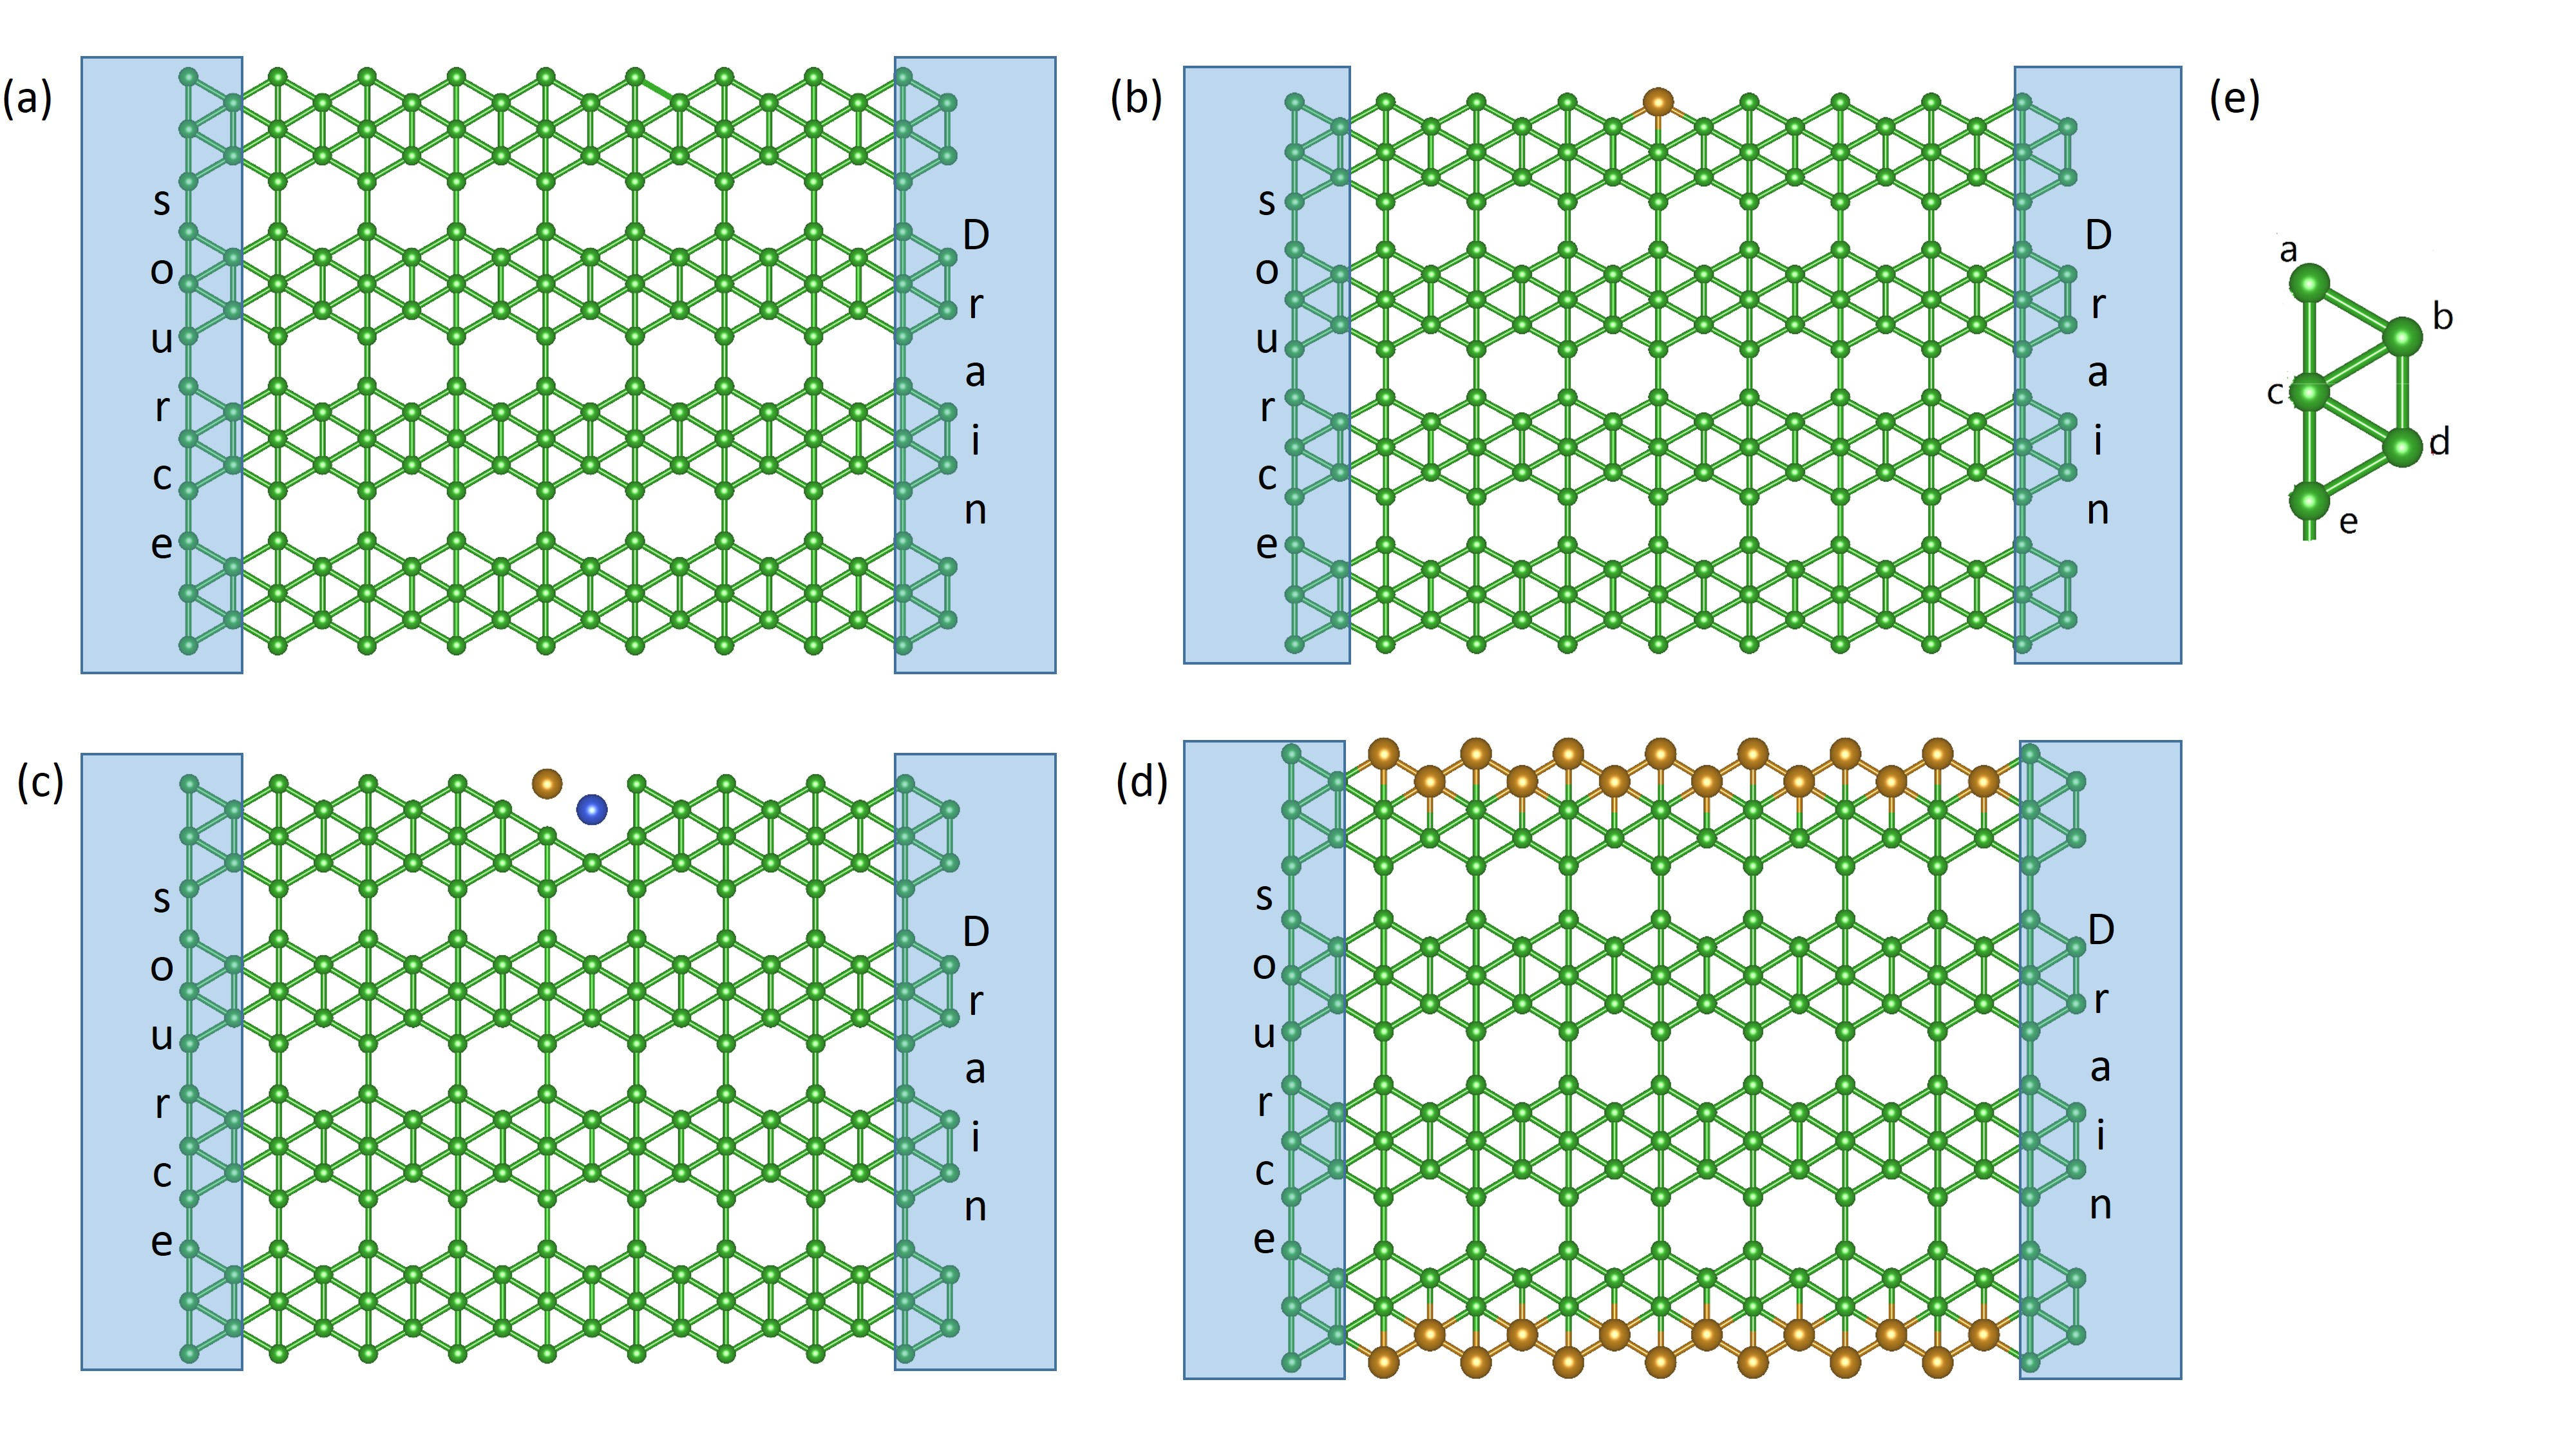
\includegraphics[width=1\linewidth]{./figures/borophene_structure(3).JPG}
    \caption{(الف) شماتیک نانوروبان زیگزاگ $\beta_{12}$-بوروفن که این ساختار از یک شبکه مربعی با پایه تشکیل شده است.(ب) شماتیک یک نانوروبان زیگزاگ $\beta_{12}$-بوروفن با ناخالصی لبه پراکنده.(ج) نمودار یک نانوروبان زیگزاگ $\beta_{12}$-بوروفن با یک و دو جای خالی در لبه.(د) شماتیک نانوروبان زیگزاگ $\beta_{12}$-بوروفن با اختلال لبه اندرسون.(ه) اساس شامل پنج اتم است که با \lr{a، b، c، d و e} نشان داده می شوند.}
   \label{fig:borophene}
\end{figure*}
  \begin{figure}[!ht]
    \centering
    % GNUPLOT: LaTeX picture with Postscript
\begingroup
  % Encoding inside the plot.  In the header of your document, this encoding
  % should to defined, e.g., by using
  % \usepackage[cp1252,<other encodings>]{inputenc}
  % \inputencoding{cp1252}%
  \makeatletter
  \providecommand\color[2][]{%
    \GenericError{(gnuplot) \space\space\space\@spaces}{%
      Package color not loaded in conjunction with
      terminal option `colourtext'%
    }{See the gnuplot documentation for explanation.%
    }{Either use 'blacktext' in gnuplot or load the package
      color.sty in LaTeX.}%
    \renewcommand\color[2][]{}%
  }%
  \providecommand\includegraphics[2][]{%
    \GenericError{(gnuplot) \space\space\space\@spaces}{%
      Package graphicx or graphics not loaded%
    }{See the gnuplot documentation for explanation.%
    }{The gnuplot epslatex terminal needs graphicx.sty or graphics.sty.}%
    \renewcommand\includegraphics[2][]{}%
  }%
  \providecommand\rotatebox[2]{#2}%
  \@ifundefined{ifGPcolor}{%
    \newif\ifGPcolor
    \GPcolorfalse
  }{}%
  \@ifundefined{ifGPblacktext}{%
    \newif\ifGPblacktext
    \GPblacktexttrue
  }{}%
  % define a \g@addto@macro without @ in the name:
  \let\gplgaddtomacro\g@addto@macro
  % define empty templates for all commands taking text:
  \gdef\gplbacktext{}%
  \gdef\gplfronttext{}%
  \makeatother
  \ifGPblacktext
    % no textcolor at all
    \def\colorrgb#1{}%
    \def\colorgray#1{}%
  \else
    % gray or color?
    \ifGPcolor
      \def\colorrgb#1{\color[rgb]{#1}}%
      \def\colorgray#1{\color[gray]{#1}}%
      \expandafter\def\csname LTw\endcsname{\color{white}}%
      \expandafter\def\csname LTb\endcsname{\color{black}}%
      \expandafter\def\csname LTa\endcsname{\color{black}}%
      \expandafter\def\csname LT0\endcsname{\color[rgb]{1,0,0}}%
      \expandafter\def\csname LT1\endcsname{\color[rgb]{0,1,0}}%
      \expandafter\def\csname LT2\endcsname{\color[rgb]{0,0,1}}%
      \expandafter\def\csname LT3\endcsname{\color[rgb]{1,0,1}}%
      \expandafter\def\csname LT4\endcsname{\color[rgb]{0,1,1}}%
      \expandafter\def\csname LT5\endcsname{\color[rgb]{1,1,0}}%
      \expandafter\def\csname LT6\endcsname{\color[rgb]{0,0,0}}%
      \expandafter\def\csname LT7\endcsname{\color[rgb]{1,0.3,0}}%
      \expandafter\def\csname LT8\endcsname{\color[rgb]{0.5,0.5,0.5}}%
    \else
      % gray
      \def\colorrgb#1{\color{black}}%
      \def\colorgray#1{\color[gray]{#1}}%
      \expandafter\def\csname LTw\endcsname{\color{white}}%
      \expandafter\def\csname LTb\endcsname{\color{black}}%
      \expandafter\def\csname LTa\endcsname{\color{black}}%
      \expandafter\def\csname LT0\endcsname{\color{black}}%
      \expandafter\def\csname LT1\endcsname{\color{black}}%
      \expandafter\def\csname LT2\endcsname{\color{black}}%
      \expandafter\def\csname LT3\endcsname{\color{black}}%
      \expandafter\def\csname LT4\endcsname{\color{black}}%
      \expandafter\def\csname LT5\endcsname{\color{black}}%
      \expandafter\def\csname LT6\endcsname{\color{black}}%
      \expandafter\def\csname LT7\endcsname{\color{black}}%
      \expandafter\def\csname LT8\endcsname{\color{black}}%
    \fi
  \fi
    \setlength{\unitlength}{0.0500bp}%
    \ifx\gptboxheight\undefined%
      \newlength{\gptboxheight}%
      \newlength{\gptboxwidth}%
      \newsavebox{\gptboxtext}%
    \fi%
    \setlength{\fboxrule}{0.5pt}%
    \setlength{\fboxsep}{1pt}%
\begin{picture}(4320.00,5760.00)%
    \gplgaddtomacro\gplbacktext{%
      \csname LTb\endcsname%%
      \put(300,3320){\makebox(0,0)[r]{\strut{}$0$}}%
      \put(300,3567){\makebox(0,0)[r]{\strut{}$1$}}%
      \put(300,3813){\makebox(0,0)[r]{\strut{}$2$}}%
      \put(300,4060){\makebox(0,0)[r]{\strut{}$3$}}%
      \put(300,4306){\makebox(0,0)[r]{\strut{}$4$}}%
      \put(300,4553){\makebox(0,0)[r]{\strut{}$5$}}%
      \put(300,4799){\makebox(0,0)[r]{\strut{}$6$}}%
      \put(300,5046){\makebox(0,0)[r]{\strut{}$7$}}%
      \put(300,5292){\makebox(0,0)[r]{\strut{}$8$}}%
      \put(300,5539){\makebox(0,0)[r]{\strut{}$9$}}%
      \put(432,3100){\makebox(0,0){\strut{}$-2$}}%
      \put(866,3100){\makebox(0,0){\strut{}$-1.5$}}%
      \put(1300,3100){\makebox(0,0){\strut{}$-1$}}%
      \put(1735,3100){\makebox(0,0){\strut{}$-0.5$}}%
      \put(2169,3100){\makebox(0,0){\strut{}$0$}}%
      \put(2603,3100){\makebox(0,0){\strut{}$0.5$}}%
      \put(3037,3100){\makebox(0,0){\strut{}$1$}}%
      \put(3471,3100){\makebox(0,0){\strut{}$1.5$}}%
      \put(3906,3100){\makebox(0,0){\strut{}$2$}}%
      \put(607,5428){\makebox(0,0)[l]{\strut{}(a)}}%
    }%
    \gplgaddtomacro\gplfronttext{%
      \csname LTb\endcsname%%
      \put(-52,4429){\rotatebox{-270}{\makebox(0,0){\strut{}$G/G_0$}}}%
      \csname LTb\endcsname%%
      \put(2936,5366){\makebox(0,0)[r]{\strut{}Pristine-$\beta_{12}$}}%
      \csname LTb\endcsname%%
      \put(2936,5146){\makebox(0,0)[r]{\strut{}V=1 eV}}%
      \csname LTb\endcsname%%
      \put(2936,4926){\makebox(0,0)[r]{\strut{}V=2 eV}}%
      \csname LTb\endcsname%%
      \put(2936,4706){\makebox(0,0)[r]{\strut{}V=5 eV}}%
    }%
    \gplgaddtomacro\gplbacktext{%
      \csname LTb\endcsname%%
      \put(300,704){\makebox(0,0)[r]{\strut{}$0$}}%
      \put(300,1193){\makebox(0,0)[r]{\strut{}$0.05$}}%
      \put(300,1682){\makebox(0,0)[r]{\strut{}$0.1$}}%
      \put(300,2171){\makebox(0,0)[r]{\strut{}$0.15$}}%
      \put(300,2660){\makebox(0,0)[r]{\strut{}$0.2$}}%
      \put(432,484){\makebox(0,0){\strut{}$-2$}}%
      \put(866,484){\makebox(0,0){\strut{}$-1.5$}}%
      \put(1300,484){\makebox(0,0){\strut{}$-1$}}%
      \put(1735,484){\makebox(0,0){\strut{}$-0.5$}}%
      \put(2169,484){\makebox(0,0){\strut{}$0$}}%
      \put(2603,484){\makebox(0,0){\strut{}$0.5$}}%
      \put(3037,484){\makebox(0,0){\strut{}$1$}}%
      \put(3471,484){\makebox(0,0){\strut{}$1.5$}}%
      \put(3906,484){\makebox(0,0){\strut{}$2$}}%
      \put(607,2562){\makebox(0,0)[l]{\strut{}(b)}}%
    }%
    \gplgaddtomacro\gplfronttext{%
      \csname LTb\endcsname%%
      \put(-448,1682){\rotatebox{-270}{\makebox(0,0){\strut{}LDOS}}}%
      \put(2177,154){\makebox(0,0){\strut{}Energy(eV)}}%
    }%
    \gplbacktext
    \put(0,0){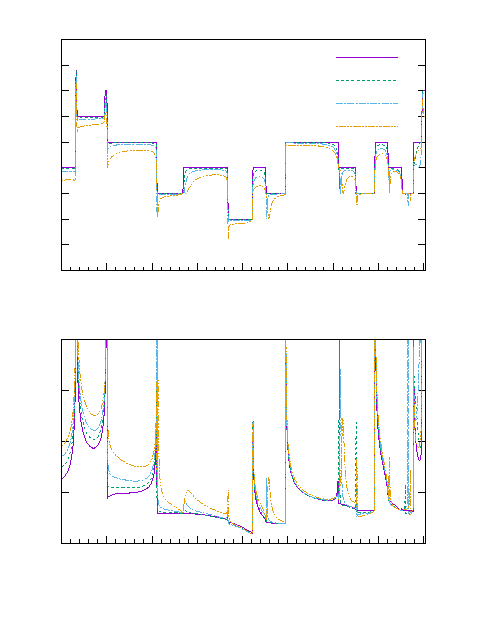
\includegraphics[width={217.00bp},height={289.00bp}]{zigscatter}}%
    \gplfronttext
  \end{picture}%
\endgroup

    \caption{الف) رسانایی نانو نوارهای زیگزاگی با عرض \lr{\AA}18.59 و طول \lr{\AA} 42.34، با ناخالصی واقع در لبه بالایی یک سوپرسل در نانو نوار. (ب) چگالی الکترونی حالات در نزدیکترین محل همسایه ناخالصی که همان a.}
    \label{zigscatter}
  \end{figure}
  \begin{figure}[ht]
    \centering
    % GNUPLOT: LaTeX picture with Postscript
\begingroup
  % Encoding inside the plot.  In the header of your document, this encoding
  % should to defined, e.g., by using
  % \usepackage[cp1252,<other encodings>]{inputenc}
  % \inputencoding{cp1252}%
  \makeatletter
  \providecommand\color[2][]{%
    \GenericError{(gnuplot) \space\space\space\@spaces}{%
      Package color not loaded in conjunction with
      terminal option `colourtext'%
    }{See the gnuplot documentation for explanation.%
    }{Either use 'blacktext' in gnuplot or load the package
      color.sty in LaTeX.}%
    \renewcommand\color[2][]{}%
  }%
  \providecommand\includegraphics[2][]{%
    \GenericError{(gnuplot) \space\space\space\@spaces}{%
      Package graphicx or graphics not loaded%
    }{See the gnuplot documentation for explanation.%
    }{The gnuplot epslatex terminal needs graphicx.sty or graphics.sty.}%
    \renewcommand\includegraphics[2][]{}%
  }%
  \providecommand\rotatebox[2]{#2}%
  \@ifundefined{ifGPcolor}{%
    \newif\ifGPcolor
    \GPcolorfalse
  }{}%
  \@ifundefined{ifGPblacktext}{%
    \newif\ifGPblacktext
    \GPblacktexttrue
  }{}%
  % define a \g@addto@macro without @ in the name:
  \let\gplgaddtomacro\g@addto@macro
  % define empty templates for all commands taking text:
  \gdef\gplbacktext{}%
  \gdef\gplfronttext{}%
  \makeatother
  \ifGPblacktext
    % no textcolor at all
    \def\colorrgb#1{}%
    \def\colorgray#1{}%
  \else
    % gray or color?
    \ifGPcolor
      \def\colorrgb#1{\color[rgb]{#1}}%
      \def\colorgray#1{\color[gray]{#1}}%
      \expandafter\def\csname LTw\endcsname{\color{white}}%
      \expandafter\def\csname LTb\endcsname{\color{black}}%
      \expandafter\def\csname LTa\endcsname{\color{black}}%
      \expandafter\def\csname LT0\endcsname{\color[rgb]{1,0,0}}%
      \expandafter\def\csname LT1\endcsname{\color[rgb]{0,1,0}}%
      \expandafter\def\csname LT2\endcsname{\color[rgb]{0,0,1}}%
      \expandafter\def\csname LT3\endcsname{\color[rgb]{1,0,1}}%
      \expandafter\def\csname LT4\endcsname{\color[rgb]{0,1,1}}%
      \expandafter\def\csname LT5\endcsname{\color[rgb]{1,1,0}}%
      \expandafter\def\csname LT6\endcsname{\color[rgb]{0,0,0}}%
      \expandafter\def\csname LT7\endcsname{\color[rgb]{1,0.3,0}}%
      \expandafter\def\csname LT8\endcsname{\color[rgb]{0.5,0.5,0.5}}%
    \else
      % gray
      \def\colorrgb#1{\color{black}}%
      \def\colorgray#1{\color[gray]{#1}}%
      \expandafter\def\csname LTw\endcsname{\color{white}}%
      \expandafter\def\csname LTb\endcsname{\color{black}}%
      \expandafter\def\csname LTa\endcsname{\color{black}}%
      \expandafter\def\csname LT0\endcsname{\color{black}}%
      \expandafter\def\csname LT1\endcsname{\color{black}}%
      \expandafter\def\csname LT2\endcsname{\color{black}}%
      \expandafter\def\csname LT3\endcsname{\color{black}}%
      \expandafter\def\csname LT4\endcsname{\color{black}}%
      \expandafter\def\csname LT5\endcsname{\color{black}}%
      \expandafter\def\csname LT6\endcsname{\color{black}}%
      \expandafter\def\csname LT7\endcsname{\color{black}}%
      \expandafter\def\csname LT8\endcsname{\color{black}}%
    \fi
  \fi
    \setlength{\unitlength}{0.0500bp}%
    \ifx\gptboxheight\undefined%
      \newlength{\gptboxheight}%
      \newlength{\gptboxwidth}%
      \newsavebox{\gptboxtext}%
    \fi%
    \setlength{\fboxrule}{0.5pt}%
    \setlength{\fboxsep}{1pt}%
\begin{picture}(4320.00,5760.00)%
    \gplgaddtomacro\gplbacktext{%
      \csname LTb\endcsname%%
      \put(300,3320){\makebox(0,0)[r]{\strut{}$0$}}%
      \put(300,3597){\makebox(0,0)[r]{\strut{}$1$}}%
      \put(300,3875){\makebox(0,0)[r]{\strut{}$2$}}%
      \put(300,4152){\makebox(0,0)[r]{\strut{}$3$}}%
      \put(300,4430){\makebox(0,0)[r]{\strut{}$4$}}%
      \put(300,4707){\makebox(0,0)[r]{\strut{}$5$}}%
      \put(300,4984){\makebox(0,0)[r]{\strut{}$6$}}%
      \put(300,5262){\makebox(0,0)[r]{\strut{}$7$}}%
      \put(300,5539){\makebox(0,0)[r]{\strut{}$8$}}%
      \put(432,3100){\makebox(0,0){\strut{}$-2$}}%
      \put(868,3100){\makebox(0,0){\strut{}$-1.5$}}%
      \put(1305,3100){\makebox(0,0){\strut{}$-1$}}%
      \put(1741,3100){\makebox(0,0){\strut{}$-0.5$}}%
      \put(2178,3100){\makebox(0,0){\strut{}$0$}}%
      \put(2614,3100){\makebox(0,0){\strut{}$0.5$}}%
      \put(3050,3100){\makebox(0,0){\strut{}$1$}}%
      \put(3487,3100){\makebox(0,0){\strut{}$1.5$}}%
      \put(3923,3100){\makebox(0,0){\strut{}$2$}}%
      \put(676,5428){\makebox(0,0)[l]{\strut{}(a)}}%
    }%
    \gplgaddtomacro\gplfronttext{%
      \csname LTb\endcsname%%
      \put(-52,4429){\rotatebox{-270}{\makebox(0,0){\strut{}$G/G_0$}}}%
      \csname LTb\endcsname%%
      \put(2936,5366){\makebox(0,0)[r]{\strut{}Pristine-$\beta_{12}$}}%
      \csname LTb\endcsname%%
      \put(2936,5146){\makebox(0,0)[r]{\strut{}V=1 eV}}%
      \csname LTb\endcsname%%
      \put(2936,4926){\makebox(0,0)[r]{\strut{}V=2 eV}}%
      \csname LTb\endcsname%%
      \put(2936,4706){\makebox(0,0)[r]{\strut{}V=5 eV}}%
    }%
    \gplgaddtomacro\gplbacktext{%
      \csname LTb\endcsname%%
      \put(300,704){\makebox(0,0)[r]{\strut{}$0$}}%
      \put(300,1095){\makebox(0,0)[r]{\strut{}$0.1$}}%
      \put(300,1486){\makebox(0,0)[r]{\strut{}$0.2$}}%
      \put(300,1878){\makebox(0,0)[r]{\strut{}$0.3$}}%
      \put(300,2269){\makebox(0,0)[r]{\strut{}$0.4$}}%
      \put(300,2660){\makebox(0,0)[r]{\strut{}$0.5$}}%
      \put(432,484){\makebox(0,0){\strut{}$-2$}}%
      \put(868,484){\makebox(0,0){\strut{}$-1.5$}}%
      \put(1305,484){\makebox(0,0){\strut{}$-1$}}%
      \put(1741,484){\makebox(0,0){\strut{}$-0.5$}}%
      \put(2178,484){\makebox(0,0){\strut{}$0$}}%
      \put(2614,484){\makebox(0,0){\strut{}$0.5$}}%
      \put(3050,484){\makebox(0,0){\strut{}$1$}}%
      \put(3487,484){\makebox(0,0){\strut{}$1.5$}}%
      \put(3923,484){\makebox(0,0){\strut{}$2$}}%
      \put(676,2562){\makebox(0,0)[l]{\strut{}(b)}}%
    }%
    \gplgaddtomacro\gplfronttext{%
      \csname LTb\endcsname%%
      \put(-316,1682){\rotatebox{-270}{\makebox(0,0){\strut{}LDOS}}}%
      \put(2177,154){\makebox(0,0){\strut{}Energy(eV)}}%
    }%
    \gplbacktext
    \put(0,0){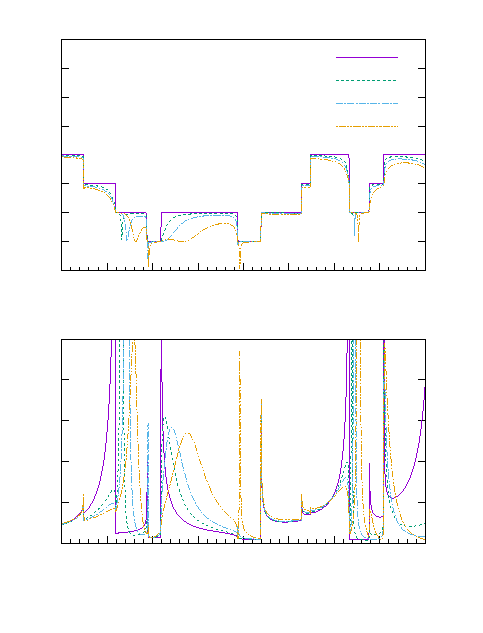
\includegraphics[width={217.00bp},height={289.00bp}]{armscatter}}%
    \gplfronttext
  \end{picture}%
\endgroup

    \caption{(الف) رسانایی نانو نوارهای آرمچیر آرمچیر با عرض \lr{\AA} 10.24 و طول \lr{\AA} 74.36 با ناخالصی واقع در لبه بالایی یک سوپرسل در نانو نوار. (ب) چگالی الکترونی حالات در نزدیکترین محل همسایه ناخالصی که همان a.}
    \label{armscatter}
  \end{figure}

\begin{figure}[ht]
    \centering
    % GNUPLOT: LaTeX picture with Postscript
\begingroup
  % Encoding inside the plot.  In the header of your document, this encoding
  % should to defined, e.g., by using
  % \usepackage[cp1252,<other encodings>]{inputenc}
  % \inputencoding{cp1252}%
  \makeatletter
  \providecommand\color[2][]{%
    \GenericError{(gnuplot) \space\space\space\@spaces}{%
      Package color not loaded in conjunction with
      terminal option `colourtext'%
    }{See the gnuplot documentation for explanation.%
    }{Either use 'blacktext' in gnuplot or load the package
      color.sty in LaTeX.}%
    \renewcommand\color[2][]{}%
  }%
  \providecommand\includegraphics[2][]{%
    \GenericError{(gnuplot) \space\space\space\@spaces}{%
      Package graphicx or graphics not loaded%
    }{See the gnuplot documentation for explanation.%
    }{The gnuplot epslatex terminal needs graphicx.sty or graphics.sty.}%
    \renewcommand\includegraphics[2][]{}%
  }%
  \providecommand\rotatebox[2]{#2}%
  \@ifundefined{ifGPcolor}{%
    \newif\ifGPcolor
    \GPcolorfalse
  }{}%
  \@ifundefined{ifGPblacktext}{%
    \newif\ifGPblacktext
    \GPblacktexttrue
  }{}%
  % define a \g@addto@macro without @ in the name:
  \let\gplgaddtomacro\g@addto@macro
  % define empty templates for all commands taking text:
  \gdef\gplbacktext{}%
  \gdef\gplfronttext{}%
  \makeatother
  \ifGPblacktext
    % no textcolor at all
    \def\colorrgb#1{}%
    \def\colorgray#1{}%
  \else
    % gray or color?
    \ifGPcolor
      \def\colorrgb#1{\color[rgb]{#1}}%
      \def\colorgray#1{\color[gray]{#1}}%
      \expandafter\def\csname LTw\endcsname{\color{white}}%
      \expandafter\def\csname LTb\endcsname{\color{black}}%
      \expandafter\def\csname LTa\endcsname{\color{black}}%
      \expandafter\def\csname LT0\endcsname{\color[rgb]{1,0,0}}%
      \expandafter\def\csname LT1\endcsname{\color[rgb]{0,1,0}}%
      \expandafter\def\csname LT2\endcsname{\color[rgb]{0,0,1}}%
      \expandafter\def\csname LT3\endcsname{\color[rgb]{1,0,1}}%
      \expandafter\def\csname LT4\endcsname{\color[rgb]{0,1,1}}%
      \expandafter\def\csname LT5\endcsname{\color[rgb]{1,1,0}}%
      \expandafter\def\csname LT6\endcsname{\color[rgb]{0,0,0}}%
      \expandafter\def\csname LT7\endcsname{\color[rgb]{1,0.3,0}}%
      \expandafter\def\csname LT8\endcsname{\color[rgb]{0.5,0.5,0.5}}%
    \else
      % gray
      \def\colorrgb#1{\color{black}}%
      \def\colorgray#1{\color[gray]{#1}}%
      \expandafter\def\csname LTw\endcsname{\color{white}}%
      \expandafter\def\csname LTb\endcsname{\color{black}}%
      \expandafter\def\csname LTa\endcsname{\color{black}}%
      \expandafter\def\csname LT0\endcsname{\color{black}}%
      \expandafter\def\csname LT1\endcsname{\color{black}}%
      \expandafter\def\csname LT2\endcsname{\color{black}}%
      \expandafter\def\csname LT3\endcsname{\color{black}}%
      \expandafter\def\csname LT4\endcsname{\color{black}}%
      \expandafter\def\csname LT5\endcsname{\color{black}}%
      \expandafter\def\csname LT6\endcsname{\color{black}}%
      \expandafter\def\csname LT7\endcsname{\color{black}}%
      \expandafter\def\csname LT8\endcsname{\color{black}}%
    \fi
  \fi
    \setlength{\unitlength}{0.0500bp}%
    \ifx\gptboxheight\undefined%
      \newlength{\gptboxheight}%
      \newlength{\gptboxwidth}%
      \newsavebox{\gptboxtext}%
    \fi%
    \setlength{\fboxrule}{0.5pt}%
    \setlength{\fboxsep}{1pt}%
\begin{picture}(4320.00,5760.00)%
    \gplgaddtomacro\gplbacktext{%
      \csname LTb\endcsname%%
      \put(300,3320){\makebox(0,0)[r]{\strut{}$0$}}%
      \put(300,3597){\makebox(0,0)[r]{\strut{}$1$}}%
      \put(300,3875){\makebox(0,0)[r]{\strut{}$2$}}%
      \put(300,4152){\makebox(0,0)[r]{\strut{}$3$}}%
      \put(300,4430){\makebox(0,0)[r]{\strut{}$4$}}%
      \put(300,4707){\makebox(0,0)[r]{\strut{}$5$}}%
      \put(300,4984){\makebox(0,0)[r]{\strut{}$6$}}%
      \put(300,5262){\makebox(0,0)[r]{\strut{}$7$}}%
      \put(300,5539){\makebox(0,0)[r]{\strut{}$8$}}%
      \put(432,3100){\makebox(0,0){\strut{}$-2$}}%
      \put(866,3100){\makebox(0,0){\strut{}$-1.5$}}%
      \put(1300,3100){\makebox(0,0){\strut{}$-1$}}%
      \put(1735,3100){\makebox(0,0){\strut{}$-0.5$}}%
      \put(2169,3100){\makebox(0,0){\strut{}$0$}}%
      \put(2603,3100){\makebox(0,0){\strut{}$0.5$}}%
      \put(3037,3100){\makebox(0,0){\strut{}$1$}}%
      \put(3471,3100){\makebox(0,0){\strut{}$1.5$}}%
      \put(3906,3100){\makebox(0,0){\strut{}$2$}}%
      \put(676,5428){\makebox(0,0)[l]{\strut{}(a)}}%
    }%
    \gplgaddtomacro\gplfronttext{%
      \csname LTb\endcsname%%
      \put(-52,4429){\rotatebox{-270}{\makebox(0,0){\strut{}$G/G_0$}}}%
      \csname LTb\endcsname%%
      \put(2936,5366){\makebox(0,0)[r]{\strut{}Pristine-$\beta_{12}$}}%
      \csname LTb\endcsname%%
      \put(2936,5146){\makebox(0,0)[r]{\strut{}One edge Vacancy}}%
      \csname LTb\endcsname%%
      \put(2936,4926){\makebox(0,0)[r]{\strut{}Two edges Vacancies}}%
    }%
    \gplgaddtomacro\gplbacktext{%
      \csname LTb\endcsname%%
      \put(300,704){\makebox(0,0)[r]{\strut{}$0$}}%
      \put(300,1095){\makebox(0,0)[r]{\strut{}$0.1$}}%
      \put(300,1486){\makebox(0,0)[r]{\strut{}$0.2$}}%
      \put(300,1878){\makebox(0,0)[r]{\strut{}$0.3$}}%
      \put(300,2269){\makebox(0,0)[r]{\strut{}$0.4$}}%
      \put(300,2660){\makebox(0,0)[r]{\strut{}$0.5$}}%
      \put(432,484){\makebox(0,0){\strut{}$-2$}}%
      \put(868,484){\makebox(0,0){\strut{}$-1.5$}}%
      \put(1305,484){\makebox(0,0){\strut{}$-1$}}%
      \put(1741,484){\makebox(0,0){\strut{}$-0.5$}}%
      \put(2178,484){\makebox(0,0){\strut{}$0$}}%
      \put(2614,484){\makebox(0,0){\strut{}$0.5$}}%
      \put(3050,484){\makebox(0,0){\strut{}$1$}}%
      \put(3487,484){\makebox(0,0){\strut{}$1.5$}}%
      \put(3923,484){\makebox(0,0){\strut{}$2$}}%
      \put(676,2562){\makebox(0,0)[l]{\strut{}(b)}}%
    }%
    \gplgaddtomacro\gplfronttext{%
      \csname LTb\endcsname%%
      \put(-316,1682){\rotatebox{-270}{\makebox(0,0){\strut{}LDOS}}}%
      \put(2177,154){\makebox(0,0){\strut{}Energy(eV)}}%
    }%
    \gplbacktext
    \put(0,0){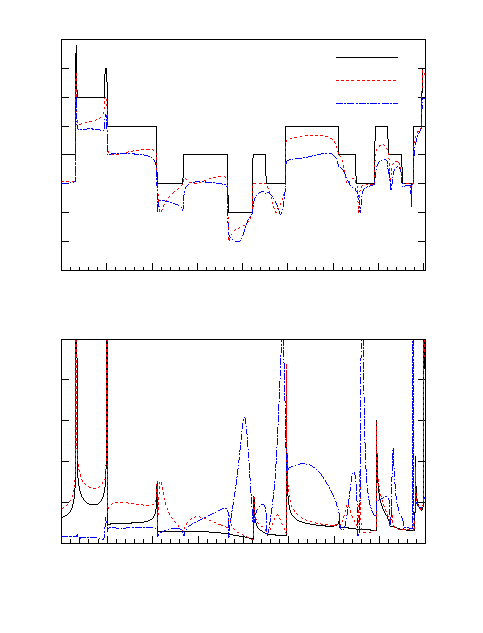
\includegraphics[width={217.00bp},height={289.00bp}]{zigvacancy}}%
    \gplfronttext
  \end{picture}%
\endgroup

    \caption{(الف) رسانایی نانو نوارهای زیگزاگی با a
    عرض \lr{\AA} 18.59 و طول \lr{\AA} 42.34، با جاهای خالی در لبه بالایی سوپرسل میانی قرار دارد.(ب) چگالی الکترونی حالات در نزدیکترین محل همسایه جاهای خالی واقع در همان (a).}
    \label{zigvacancy}
  \end{figure}
  
\begin{figure}[ht]
\centering
% GNUPLOT: LaTeX picture with Postscript
\begin{latin}
\begingroup
  \makeatletter
  \providecommand\color[2][]{%
    \GenericError{(gnuplot) \space\space\space\@spaces}{%
      Package color not loaded in conjunction with
      terminal option `colourtext'%
    }{See the gnuplot documentation for explanation.%
    }{Either use 'blacktext' in gnuplot or load the package
      color.sty in LaTeX.}%
    \renewcommand\color[2][]{}%
  }%
  \providecommand\includegraphics[2][]{%
    \GenericError{(gnuplot) \space\space\space\@spaces}{%
      Package graphicx or graphics not loaded%
    }{See the gnuplot documentation for explanation.%
    }{The gnuplot epslatex terminal needs graphicx.sty or graphics.sty.}%
    \renewcommand\includegraphics[2][]{}%
  }%
  \providecommand\rotatebox[2]{#2}%
  \@ifundefined{ifGPcolor}{%
    \newif\ifGPcolor
    \GPcolorfalse
  }{}%
  \@ifundefined{ifGPblacktext}{%
    \newif\ifGPblacktext
    \GPblacktexttrue
  }{}%
  % define a \g@addto@macro without @ in the name:
  \let\gplgaddtomacro\g@addto@macro
  % define empty templates for all commands taking text:
  \gdef\gplbacktext{}%
  \gdef\gplfronttext{}%
  \makeatother
  \ifGPblacktext
    % no textcolor at all
    \def\colorrgb#1{}%
    \def\colorgray#1{}%
  \else
    % gray or color?
    \ifGPcolor
      \def\colorrgb#1{\color[rgb]{#1}}%
      \def\colorgray#1{\color[gray]{#1}}%
      \expandafter\def\csname LTw\endcsname{\color{white}}%
      \expandafter\def\csname LTb\endcsname{\color{black}}%
      \expandafter\def\csname LTa\endcsname{\color{black}}%
      \expandafter\def\csname LT0\endcsname{\color[rgb]{1,0,0}}%
      \expandafter\def\csname LT1\endcsname{\color[rgb]{0,1,0}}%
      \expandafter\def\csname LT2\endcsname{\color[rgb]{0,0,1}}%
      \expandafter\def\csname LT3\endcsname{\color[rgb]{1,0,1}}%
      \expandafter\def\csname LT4\endcsname{\color[rgb]{0,1,1}}%
      \expandafter\def\csname LT5\endcsname{\color[rgb]{1,1,0}}%
      \expandafter\def\csname LT6\endcsname{\color[rgb]{0,0,0}}%
      \expandafter\def\csname LT7\endcsname{\color[rgb]{1,0.3,0}}%
      \expandafter\def\csname LT8\endcsname{\color[rgb]{0.5,0.5,0.5}}%
    \else
      % gray
      \def\colorrgb#1{\color{black}}%
      \def\colorgray#1{\color[gray]{#1}}%
      \expandafter\def\csname LTw\endcsname{\color{white}}%
      \expandafter\def\csname LTb\endcsname{\color{black}}%
      \expandafter\def\csname LTa\endcsname{\color{black}}%
      \expandafter\def\csname LT0\endcsname{\color{black}}%
      \expandafter\def\csname LT1\endcsname{\color{black}}%
      \expandafter\def\csname LT2\endcsname{\color{black}}%
      \expandafter\def\csname LT3\endcsname{\color{black}}%
      \expandafter\def\csname LT4\endcsname{\color{black}}%
      \expandafter\def\csname LT5\endcsname{\color{black}}%
      \expandafter\def\csname LT6\endcsname{\color{black}}%
      \expandafter\def\csname LT7\endcsname{\color{black}}%
      \expandafter\def\csname LT8\endcsname{\color{black}}%
    \fi
  \fi
    \setlength{\unitlength}{0.0500bp}%
    \ifx\gptboxheight\undefined%
      \newlength{\gptboxheight}%
      \newlength{\gptboxwidth}%
      \newsavebox{\gptboxtext}%
    \fi%
    \setlength{\fboxrule}{0.5pt}%
    \setlength{\fboxsep}{1pt}%
\begin{picture}(4320.00,5760.00)%
    \gplgaddtomacro\gplbacktext{%
      \csname LTb\endcsname%%
      \put(300,3320){\makebox(0,0)[r]{\strut{}$0$}}%
      \put(300,3597){\makebox(0,0)[r]{\strut{}$1$}}%
      \put(300,3875){\makebox(0,0)[r]{\strut{}$2$}}%
      \put(300,4152){\makebox(0,0)[r]{\strut{}$3$}}%
      \put(300,4430){\makebox(0,0)[r]{\strut{}$4$}}%
      \put(300,4707){\makebox(0,0)[r]{\strut{}$5$}}%
      \put(300,4984){\makebox(0,0)[r]{\strut{}$6$}}%
      \put(300,5262){\makebox(0,0)[r]{\strut{}$7$}}%
      \put(300,5539){\makebox(0,0)[r]{\strut{}$8$}}%
      \put(432,3100){\makebox(0,0){\strut{}$-2$}}%
      \put(868,3100){\makebox(0,0){\strut{}$-1.5$}}%
      \put(1305,3100){\makebox(0,0){\strut{}$-1$}}%
      \put(1741,3100){\makebox(0,0){\strut{}$-0.5$}}%
      \put(2178,3100){\makebox(0,0){\strut{}$0$}}%
      \put(2614,3100){\makebox(0,0){\strut{}$0.5$}}%
      \put(3050,3100){\makebox(0,0){\strut{}$1$}}%
      \put(3487,3100){\makebox(0,0){\strut{}$1.5$}}%
      \put(3923,3100){\makebox(0,0){\strut{}$2$}}%
      \put(711,5428){\makebox(0,0)[l]{\strut{}(a)}}%
    }%
    \gplgaddtomacro\gplfronttext{%
      \csname LTb\endcsname%%
      \put(-52,4429){\rotatebox{-270}{\makebox(0,0){\strut{}$G/G_0$}}}%
      \csname LTb\endcsname%%
      \put(2936,5366){\makebox(0,0)[r]{\strut{}Pristine-$\beta_{12}$}}%
      \csname LTb\endcsname%%
      \put(2936,5146){\makebox(0,0)[r]{\strut{}One edge Vacancy}}%
      \csname LTb\endcsname%%
      \put(2936,4926){\makebox(0,0)[r]{\strut{}Two edges Vacancies}}%
    }%
    \gplgaddtomacro\gplbacktext{%
      \csname LTb\endcsname%%
      \put(300,704){\makebox(0,0)[r]{\strut{}$0$}}%
      \put(300,1095){\makebox(0,0)[r]{\strut{}$0.2$}}%
      \put(300,1486){\makebox(0,0)[r]{\strut{}$0.4$}}%
      \put(300,1878){\makebox(0,0)[r]{\strut{}$0.6$}}%
      \put(300,2269){\makebox(0,0)[r]{\strut{}$0.8$}}%
      \put(300,2660){\makebox(0,0)[r]{\strut{}$1$}}%
      \put(432,484){\makebox(0,0){\strut{}$-2$}}%
      \put(868,484){\makebox(0,0){\strut{}$-1.5$}}%
      \put(1305,484){\makebox(0,0){\strut{}$-1$}}%
      \put(1741,484){\makebox(0,0){\strut{}$-0.5$}}%
      \put(2178,484){\makebox(0,0){\strut{}$0$}}%
      \put(2614,484){\makebox(0,0){\strut{}$0.5$}}%
      \put(3050,484){\makebox(0,0){\strut{}$1$}}%
      \put(3487,484){\makebox(0,0){\strut{}$1.5$}}%
      \put(3923,484){\makebox(0,0){\strut{}$2$}}%
      \put(711,2562){\makebox(0,0)[l]{\strut{}(b)}}%
    }%
    \gplgaddtomacro\gplfronttext{%
      \csname LTb\endcsname%%
      \put(-316,1682){\rotatebox{-270}{\makebox(0,0){\strut{}LDOS}}}%
      \put(2177,154){\makebox(0,0){\strut{}Energy(eV)}}%
    }%
    \gplbacktext
    \put(0,0){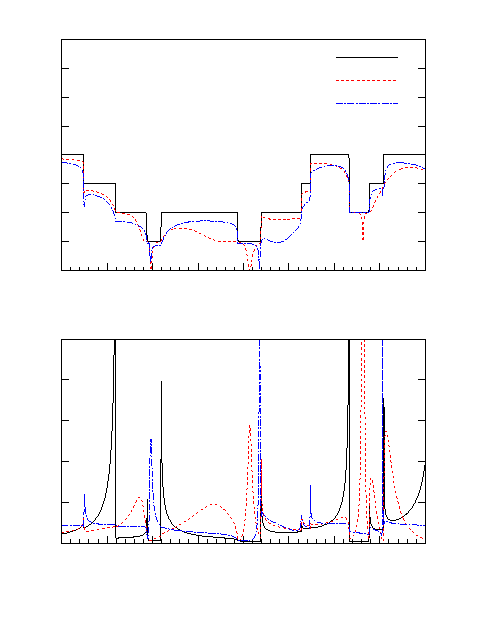
\includegraphics[width={217.00bp},height={289.00bp}]{armvacancy}}%
    \gplfronttext
  \end{picture}%
\endgroup
\end{latin}
\caption{(الف) رسانایی نانو نوارهای آرمچیر آرمچیر با a
عرض \lr{\AA} 10.24 و طول \lr{\AA} 74.36، با جاهای خالی واقع در لبه بالایی سوپرسل میانی از نانوروبان. (ب) چگالی الکترونی حالات در نزدیکترین محل همسایه جاهای خالی واقع مشابه (a).}
\label{armvacancy}
\end{figure}
\subsection{عیوب منفرد} 
به منظور توصیف اثر عیوب لبه بر الکترونیک و ترابرد نانو نوارهای شبکه لانه زنبوری، اجازه دهید ابتدا مدلی را در مورد مشکل تک نقص مورد بحث قرار دهیم. از آنجایی که مدوله \gls{شکاف نواری} تأثیر مستقیمی بر رسانایی دارد، مطالعه مدوله رسانایی در حضور انواع عیوب که در طول ساخت وسایل الکترونیکی ممکن است، مفید است. یکی از راههای مؤثر برای تعدیل شکاف نوار و در نتیجه رسانایی، ناخالصی‌های\gls{دوپینگ} است که با تغییر توزیع فضایی توابع موج در یک سیستم کوانتومی منجر به خواص نوری و الکتریکی جدید میشود. وجود نقصهای منفرد در لبه‌های نانوروبان می‌تواند تقارن زیرشبکه را بشکند و در نتیجه بر خواص الکترونیکی و ترابرد مانند رسانایی تأثیر بگذارد. بررسی نقش این عیوب لبه منجر به درک بهتر و عمیق تری برای مطالعه سایر عیوب می شود. مشکل تک نقص در نانوروبان‌ها را می توان با اعمال یک پتانسیل به اتم لبه مدل کرد. برای تفسیر نتایج شبیه سازی، می توان از یک مدل ساده بر روی شبکه لانه زنبوری استفاده کرد. همانطور که می دانیم به دلیل تقارن انتقالی در شبکه لانه زنبوری، با حل معادله شرودینگر روی یک سلول می توان تمام خصوصیات شبکه را به دست آورد، زمانی که یک پتانسیل پراکندگی با قدرت \lr{V} به یک سلول وارد شود، این تقارن شکسته می شود. سلول های حاوی ناخالصی باید بررسی شوند. بنابراین به طور جداگانه خواص اضافی ناشی از وجود یک نقص را بررسی می‌کنیم. سلولهای داخل نانوروبان را بر اساس مکانهایشان برچسبگذاری می‌کنیم به طوری که اولین سلول را در لبه بالایی سوپرسل نانوروبان به دست میآوریم (همان سلولی که پتانسیل اضافی را روی آن قرار داده‌ایم). در محل مربوط به $r = 0$ معادله شرودینگر نوشته شده است به صورت:
\begin{equation}
  \left(
  \begin{array}{cc}
    V\delta(r)&\epsilon^{*}_{k}\\
    \epsilon_k & 0
  \end{array}
  \right)
  \left(
  \begin{array}{c}
    \phi_{A}(r)\\
    \phi_{B}(r)
  \end{array}
  \right)
  =E
  \left(
  \begin{array}{c}
    \phi_{A}(r)\\
    \phi_{B}(r)
  \end{array}
  \right),
\end{equation}
جایی که $\epsilon_k$ به ساختار توری وابسته است و انرژی جهش از مکان a به مکان b در سلول واحد را تعیین می کند، با استفاده از روش استاندارد Koster-Slater%\cite{Koster1954Wave}،
% معادله خودسازگاری را که انرژی حالت را تعیین می کند، به دست می آوریم."
\begin{equation}
  \frac{1}{V}=\frac{E}{2\pi^2}\int_{1st BZ}dk\frac{1}{E^2-|\epsilon_k|^2},
  \label{virtual}
\end{equation}

\begin{figure}[!ht]
\centering
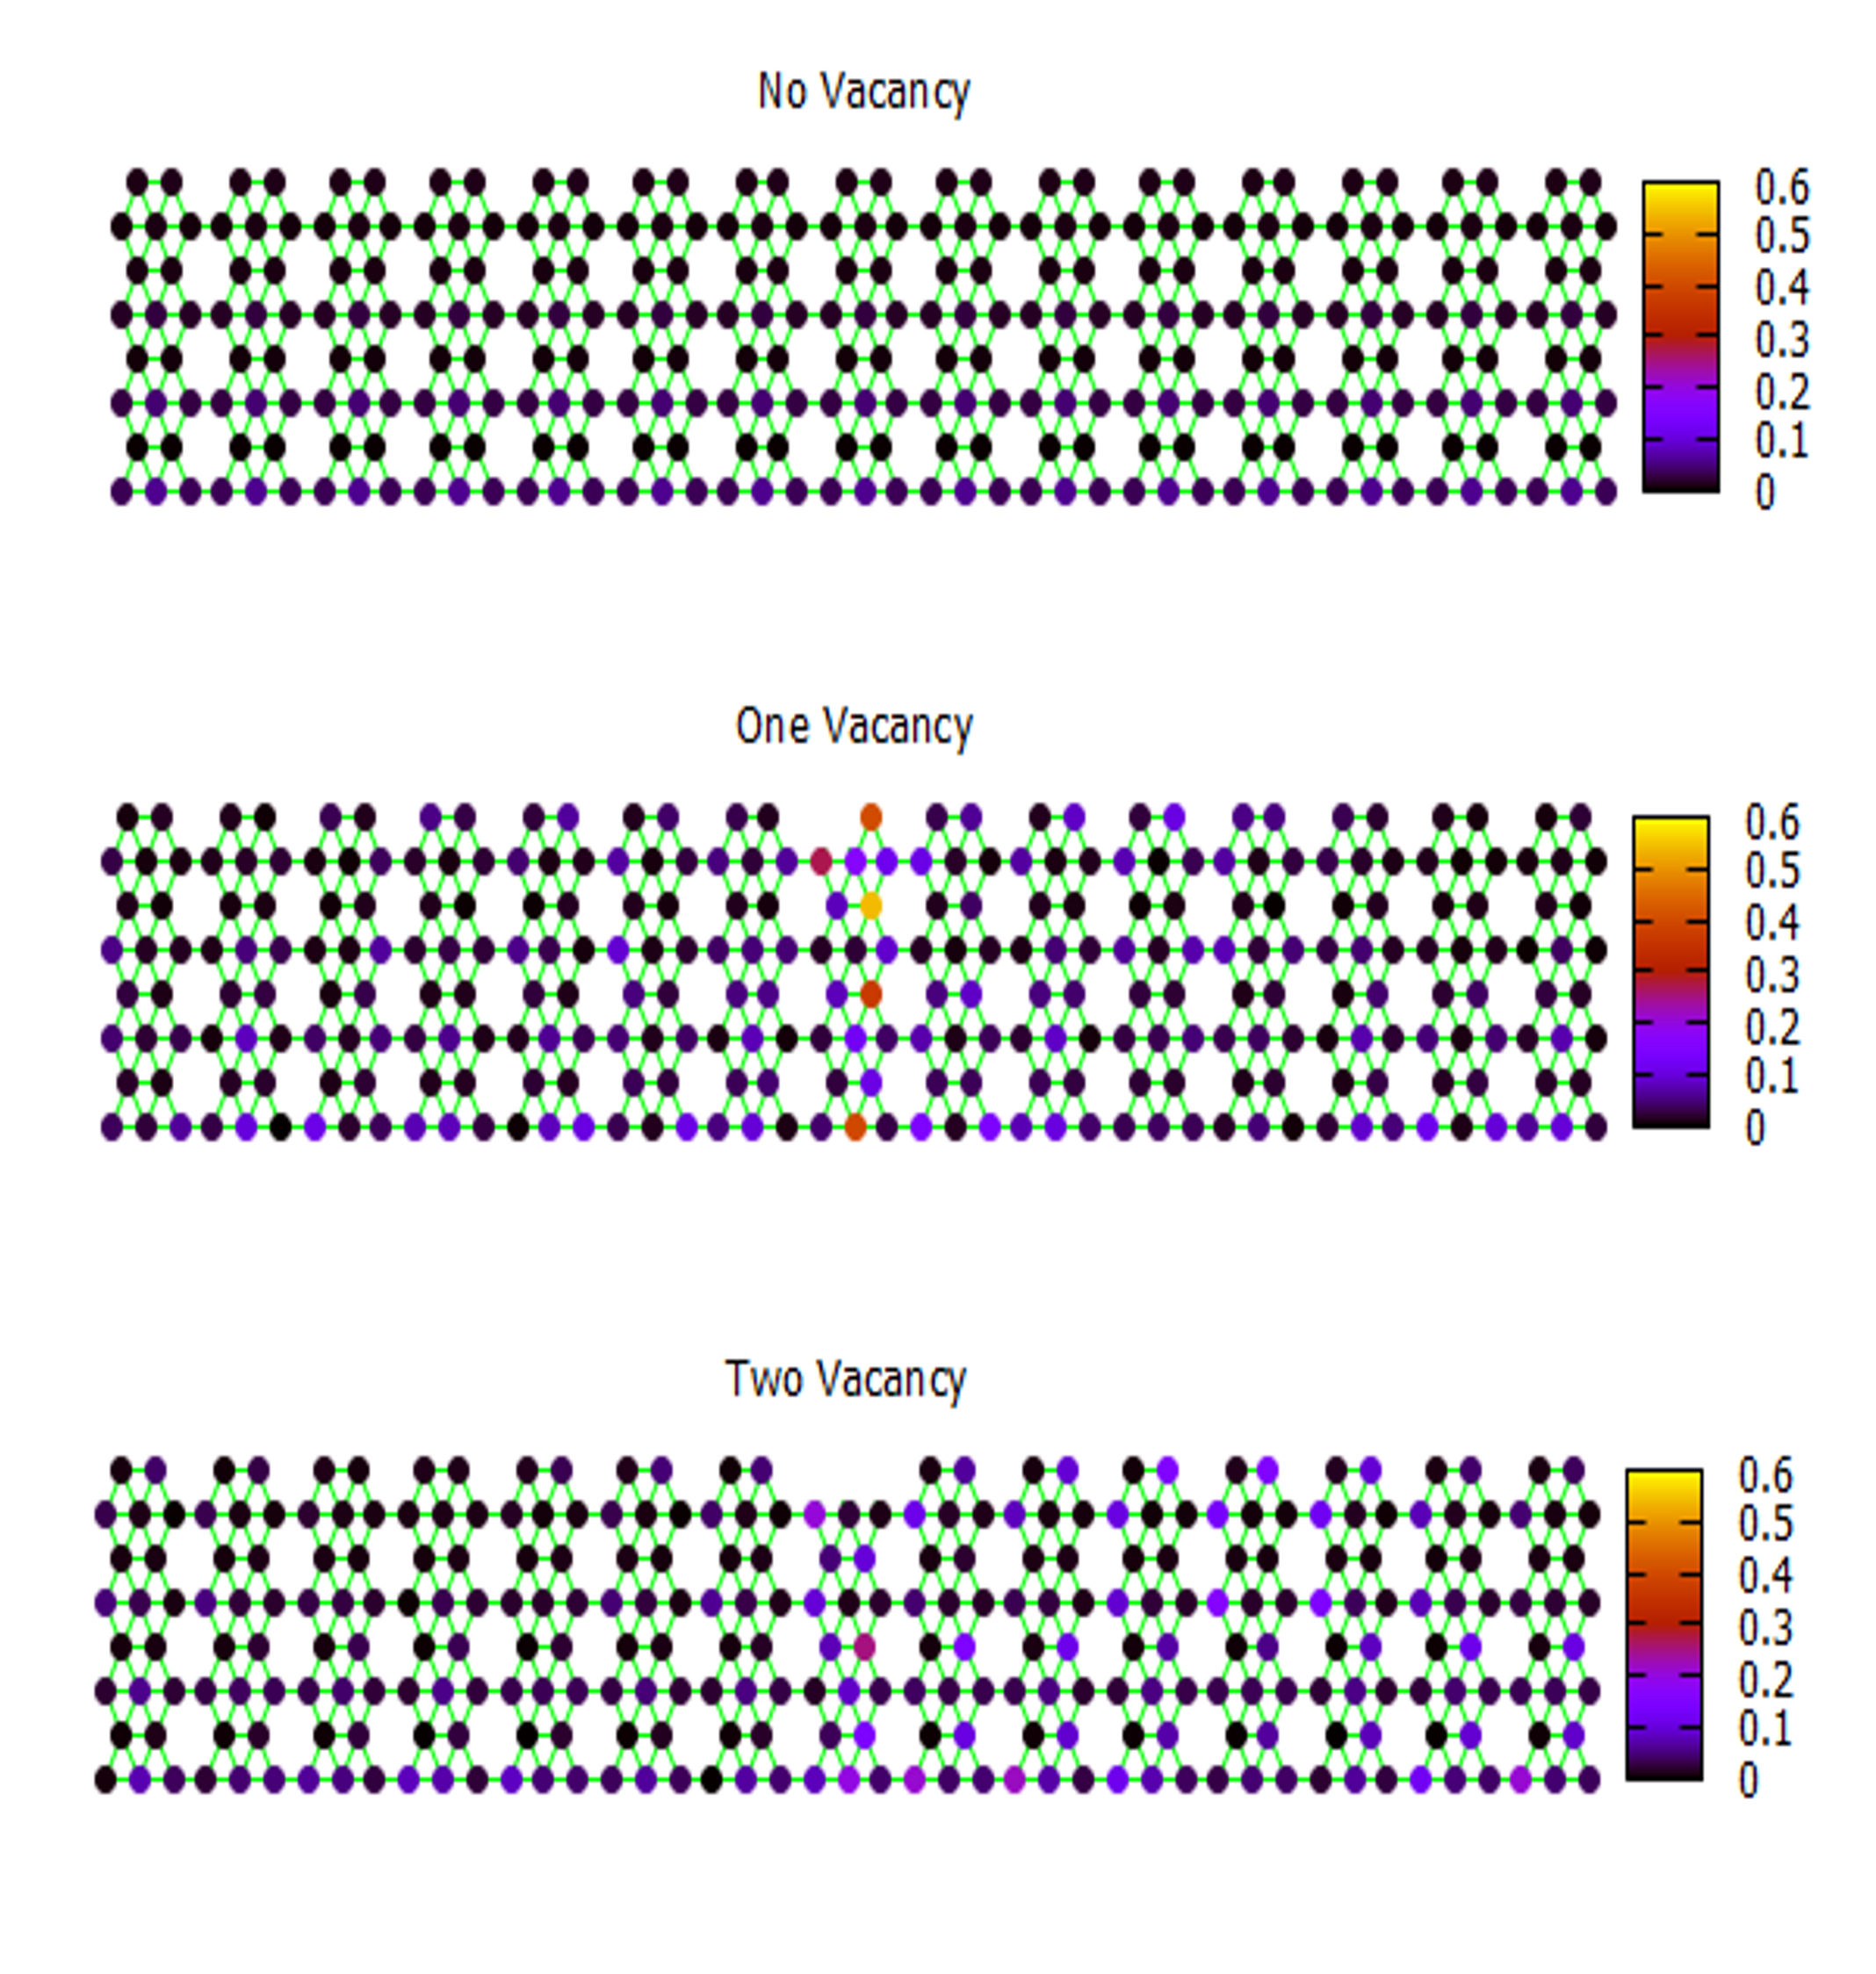
\includegraphics[width=1\linewidth]{./figures/Slide5.PNG}
\caption{در انرژی مربوط به اوج LDOS در نزدیکی انرژی فرمی، چگالی الکترونی فضایی حالات در کل محل نانوروبان بوروفن آرمچیر با یک محل خالی در لبه بالایی خالی، یک جای خالی، و دو جای خالی در وسط رسم شد. از نانو روبان}
\label{armVSLDOS}
\end{figure}
%%%% بنظر میرسد داشتن یک تصویر شماتیک برای این مبحث ضروری است که از مقاله واکی بایاشی بایدگرفت
در اینجا جهت تغییر ناپذیر انتقالی محور زیگزاگ را به عنوان محور x و محور y را عمود بر محور x در نظر می گیریم. این انتگرال عموماً یک عدد مختلط است، به این معنی که حالت کران تشدید می شود، یا به عبارت دیگر، یک حالت کران مجازی وجود دارد. برای نوارهای آرمچیر با عرض \lr{\AA}18.59 و با بی نظمی توزیع شده در هر دو لبه در طول \lr{\AA}758.81 با اختلال نسبتاً ضعیف $V_d = 1 eV$، \lr{BNR} های آرمچیر از فلز به نیمه هادی تبدیل می شوند. با یک عمر محدود در حد پتانسیل نامتناهی \lr{V} (یعنی یک جای خالی واحد در \lr{BNR}ها)، حالت کران مجازی به یک حالت کران کاملاً تعریف شده تبدیل می شود (با طول عمر نامحدود)، و سطح انرژی ناخالصی در $E = 0$ رخ می دهد. معادله شرودینگر را می‌توان برای به دست آوردن حالت ویژه در فضای \lr{k} با استفاده از این واقعیت که چگالی حالات برای یک سیستم دو بعدی با انرژی متناسب است استفاده کرد:
\begin{subequations}
  \begin{eqnarray}
    \phi_{Ak}&=\frac{V}{L^2}G_A^0\frac{E}{E^2-|\epsilon_k|^2},\\
    \phi_{Bk}&=\frac{V}{L^2}G_A^0\frac{\color{yellow}{\epsilon_k}}{E^2-|\epsilon_k|^2},
  \end{eqnarray}
  \label{}
  \end{subequations}
که در آن $G^0_A =\Sigma_k \phi_{Ak}$ با نرمال کردن توابع موج، متوجه می شویم که آنها دارای ویژگی غیرمحدود هستند، به عنوان مثال $\phi_{A}(r) = 0$ و $\phi_{B}(r)\neq 0$. بنابراین، هنگامی که یک جای خالی روی شبکه لانه زنبوری ایجاد می شود، سطح انرژی جای خالی در $E = 0$ با تابع موجی ظاهر می شود که دارای یک کاراکتر غیرمحدود است، یعنی دامنه آن در سایت \lr{a(b)} صفر است. همانطور که با معادله\ref{virtual} مشاهده می شود، وجود جاهای خالی باعث سطح انرژی $E = 0$ می شود. از سوی دیگر، نشان داده شده است که حالت های لبه فقط در نانوروبان های زیگزاگ وجود دارد و نه در آرمچیر. مشخص شده است که حالت های لبه را می توان به ترتیب در شکاف نوار یا شکاف نوار جایگزیده در نیمه هادی‌ها و هادی‌ها نیز یافت [58]. علاوه بر این، در نانوروبان‌های زیگزاگ، دو سطح انرژی در شکاف نوار وجود دارد که میتوانند با هم جفت شوند و باعث فرورفتگی رسانایی شوند، در حالی که برای نانوروبان‌های آرمچیر، هیچ کوپلینگی وجود ندارد. انرژی این افت های رسانایی مطابق با پیکربندی های ضد پیوند [60] است. بر اساس مدل فوق، اکنون ممکن است اثر یک نقص را بر رسانایی یک \lr{BNR} به صورت کمی بررسی کنیم. محاسبات عددی ما \lr{LDOS} تقریباً صفر را در محل پراکندگی نشان میدهد، که مربوط به کاراکتر نامحدود مدل مورد بررسی است. شکل 2.a رسانایی نانوروبان های زیگزاگی با عرض \lr{\AA} 18.59 و طول \lr{\AA}42.34 (15 سوپرسل) را نشان می دهد، زمانی که یک ناخالصی با انواع قدرت های بالقوه در لبه بالایی سوپرسل واقع در وسط نانو نوار وجود دارد. در شکل\ref{zigvacancy}، \lr{LDOS} در نزدیکترین محل ناخالصی همسایه مانند بالا رسم شده است. همانطور که انتظار داریم، وجود ناخالصی باعث کاهش رسانایی می شود به طوری که در انرژی های خاص منجر به افت رسانایی می شود که به طور معادل با پیک در \lr{LDOS} همراه است. همانطور که قبلا ذکر شد، یک شبکه لانه زنبوری پنهان در شبکه بوروفن $\beta_{12}$ وجود دارد، بنابراین افت رسانایی، همراه با قله های \lr{LDOS}، می تواند به حالت های شبه موضعی که در مجاورت ناخالصی رخ می دهد نسبت داد
% \subsection{چگالی حالتهای فضایی}
در این رساله، رسانایی نانوروبان‌های 
آزمایش‌ها و\gls{محاسبات اصول اولیه} نشان داده‌اند که مخروطهای دیراک از اوربیتال‌های $P_z$ مشتق شده‌اند. از آنجایی که تابع موج در انرژی فرمی در محل \lr{c} دامنه ندارد، [26] این شش اتم اطراف فاز یکدیگر را خنثی می کنند، بنابراین شکل\ref{zigCSLDOS} در انرژی متناظر تا اوج \lr{LDOS} در نزدیکی انرژی فرمی، چگالی الکترونی فضایی حالتها در کل محل نانوروبان بوروفن زیگزاگ با محل پراکندگی در لبه بالایی با \lr{V=0,1,2,5} در وسط نانوروبان ترسیم شده است. 

\begin{figure}[!ht]
  \centering
  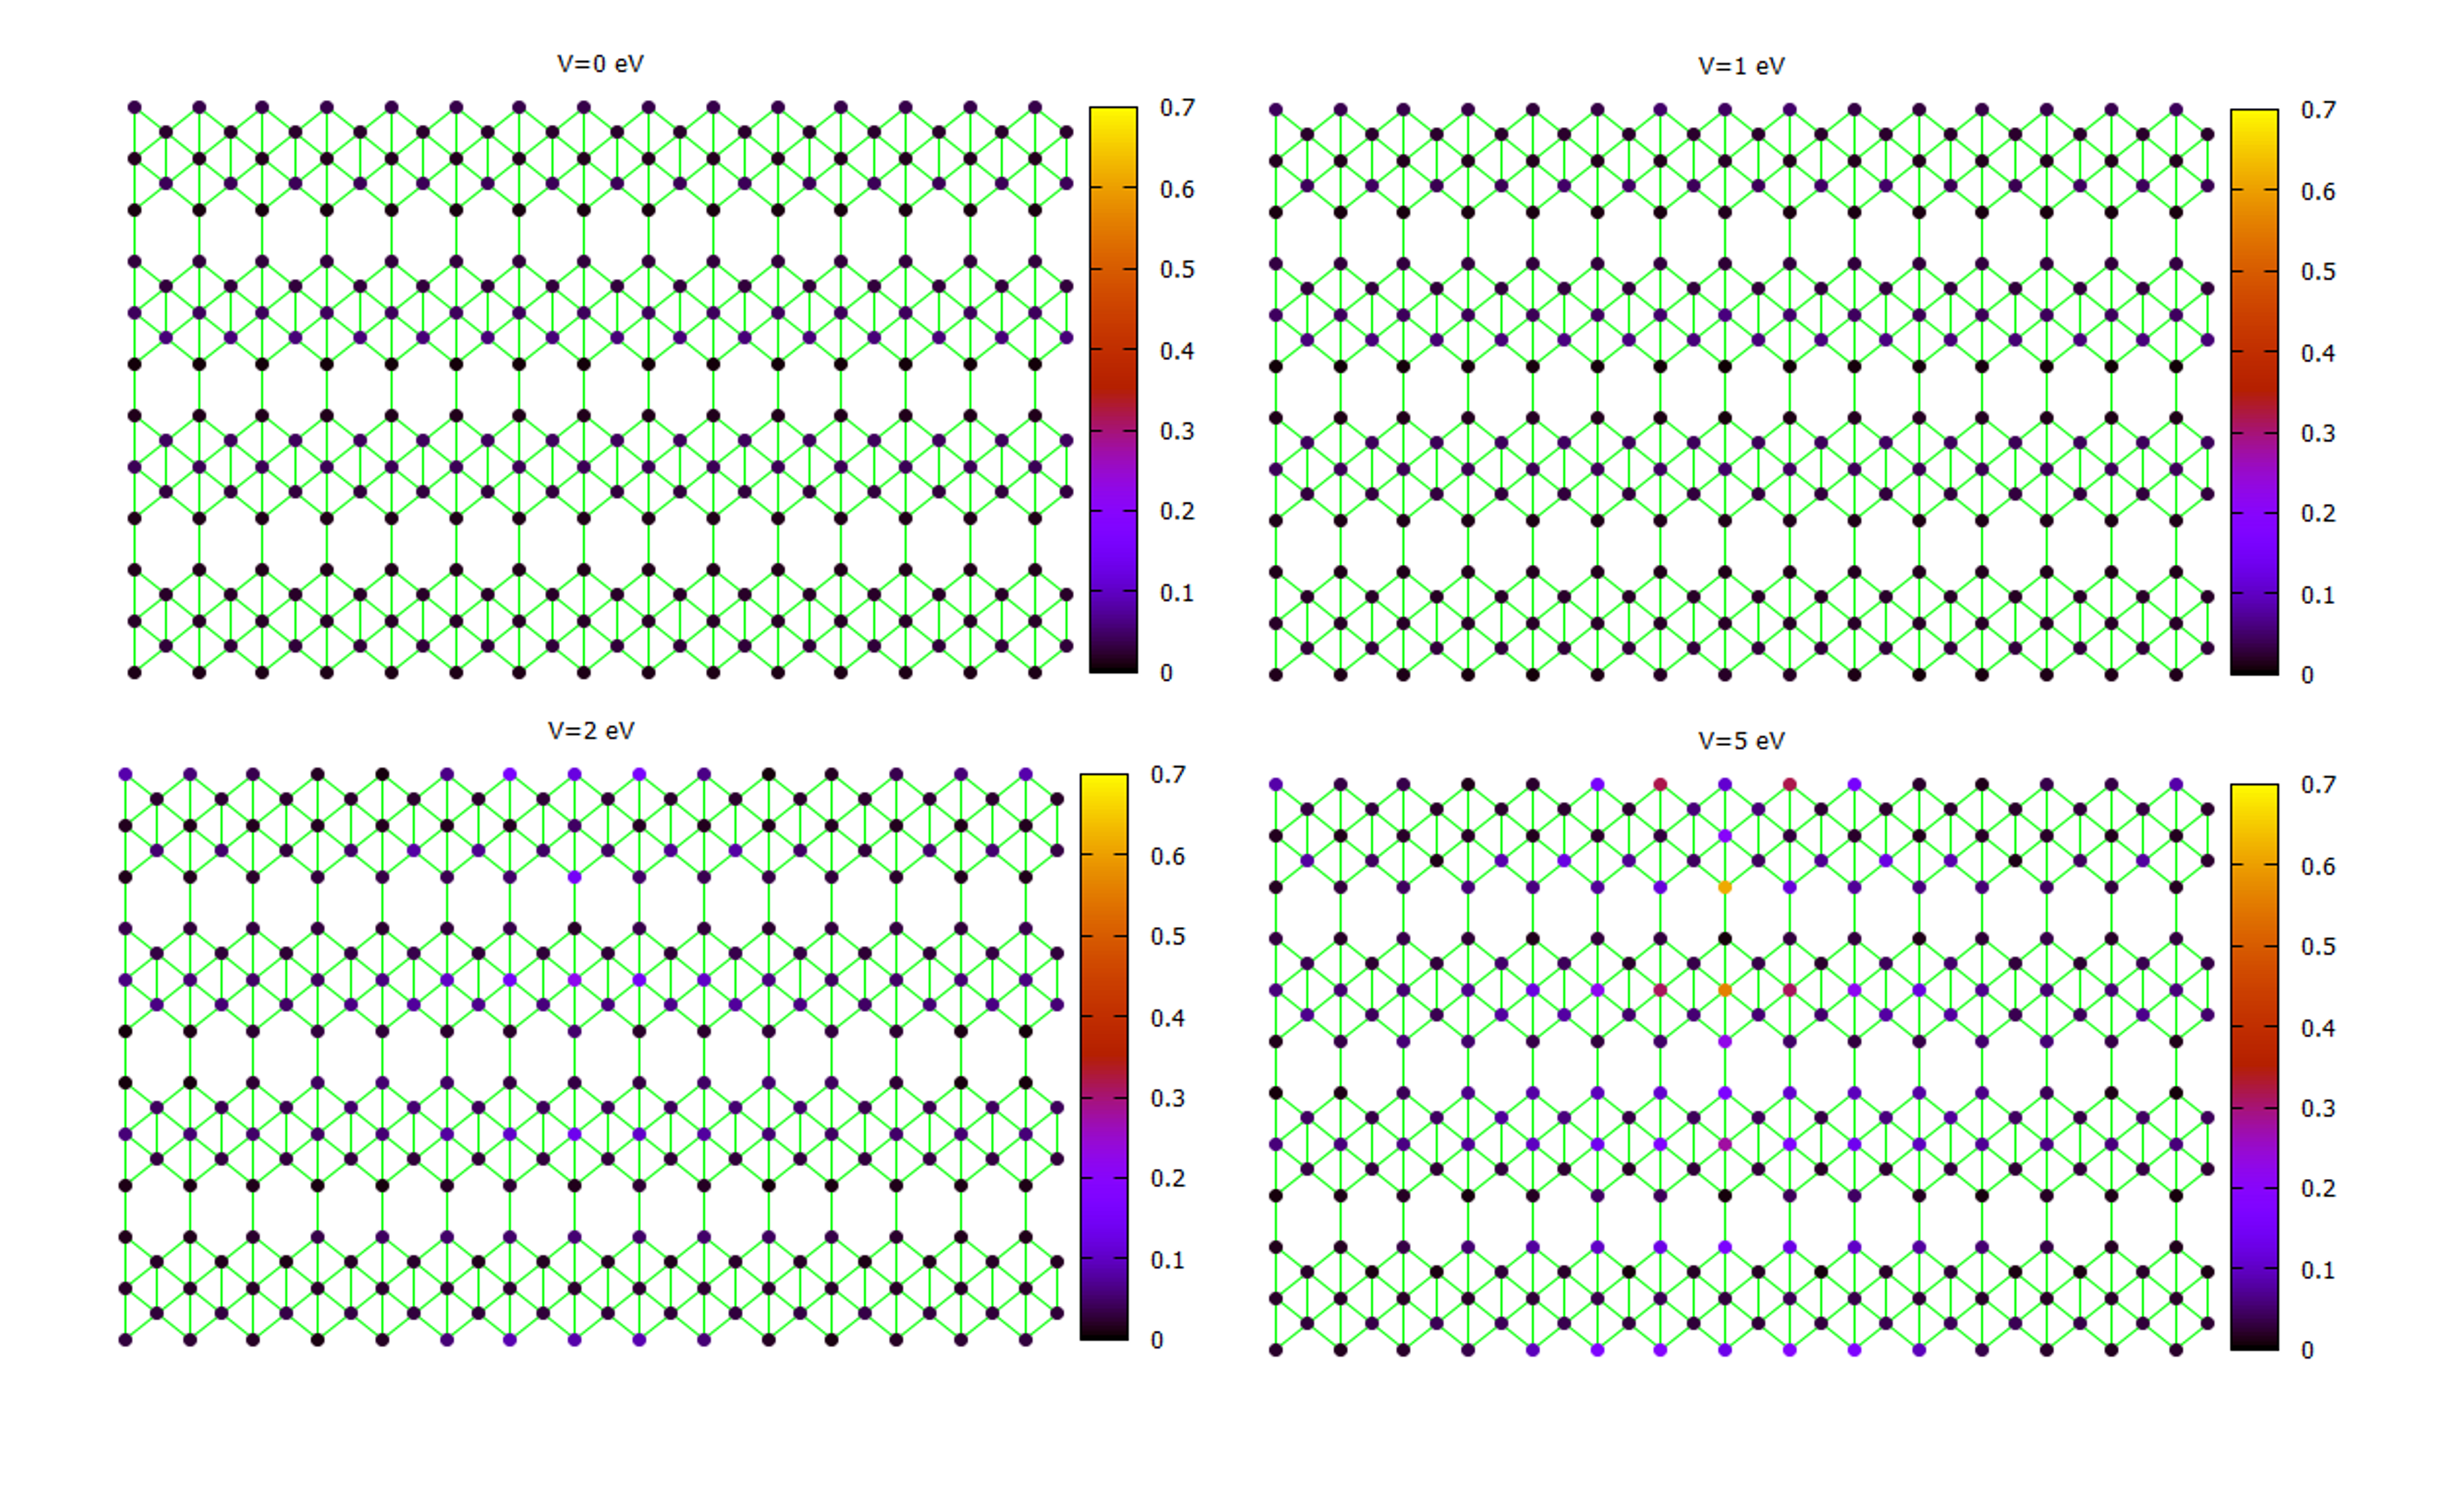
\includegraphics[width=1\linewidth]{./figures/Slide1.PNG}
  \caption{در انرژی مربوط به اوج \lr{LDOS} نزدیک انرژی فرمی، چگالی الکترونی فضایی حالات در کل محل نانوروبان بوروفن زیگزاگ با یک محل پراکندگی در لبه بالایی با \lr{V=0،1،2،5} در وسط رسم شد. از نانو روبان}
  \label{zigCSLDOS}
\end{figure}

\begin{figure}[!ht]
  \centering
  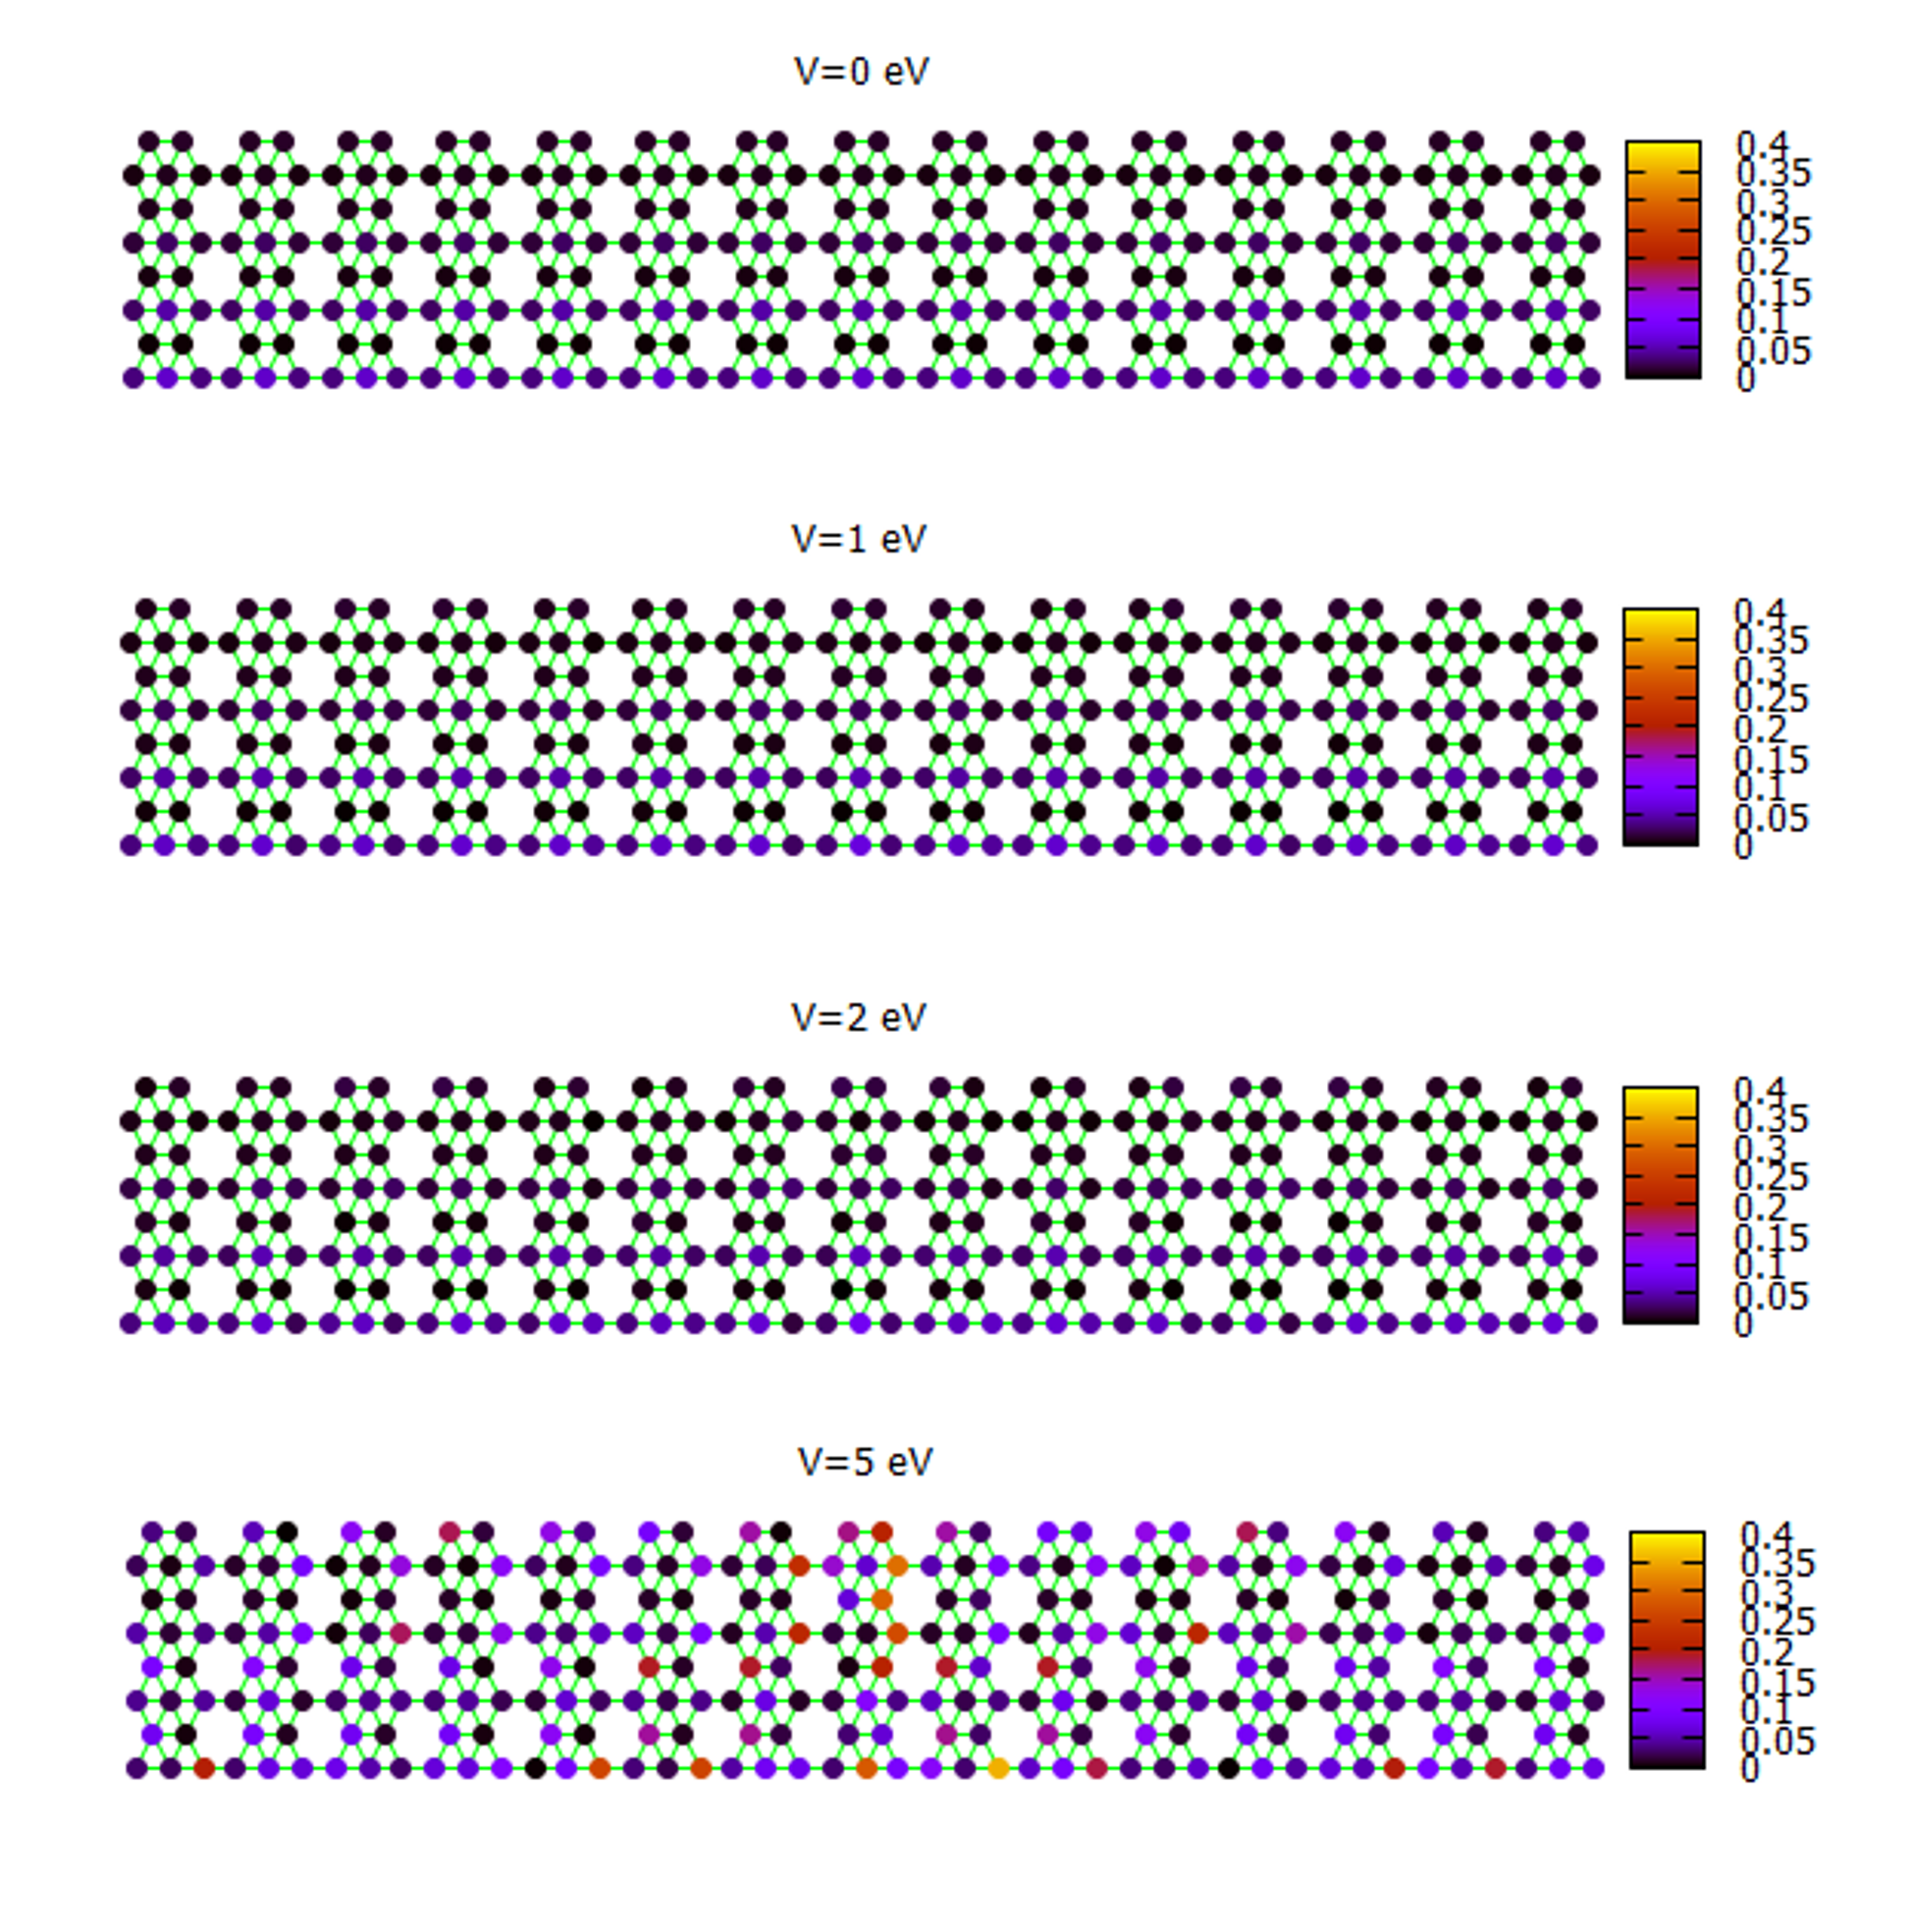
\includegraphics[width=1\linewidth]{./figures/Slide3.PNG}
  \caption{در انرژی مربوط به اوج \lr{LDOS} نزدیک انرژی فرمی، چگالی الکترونی فضایی حالات در کل محل نانوروبان بوروفن آرمچیر با یک محل پراکندگی در لبه بالایی با \lr{V=0،1،2،5} در وسط رسم شد. از نانو روبان}
  \label{armCSLDOS}
\end{figure}
\begin{figure}[!ht]
    \centering
    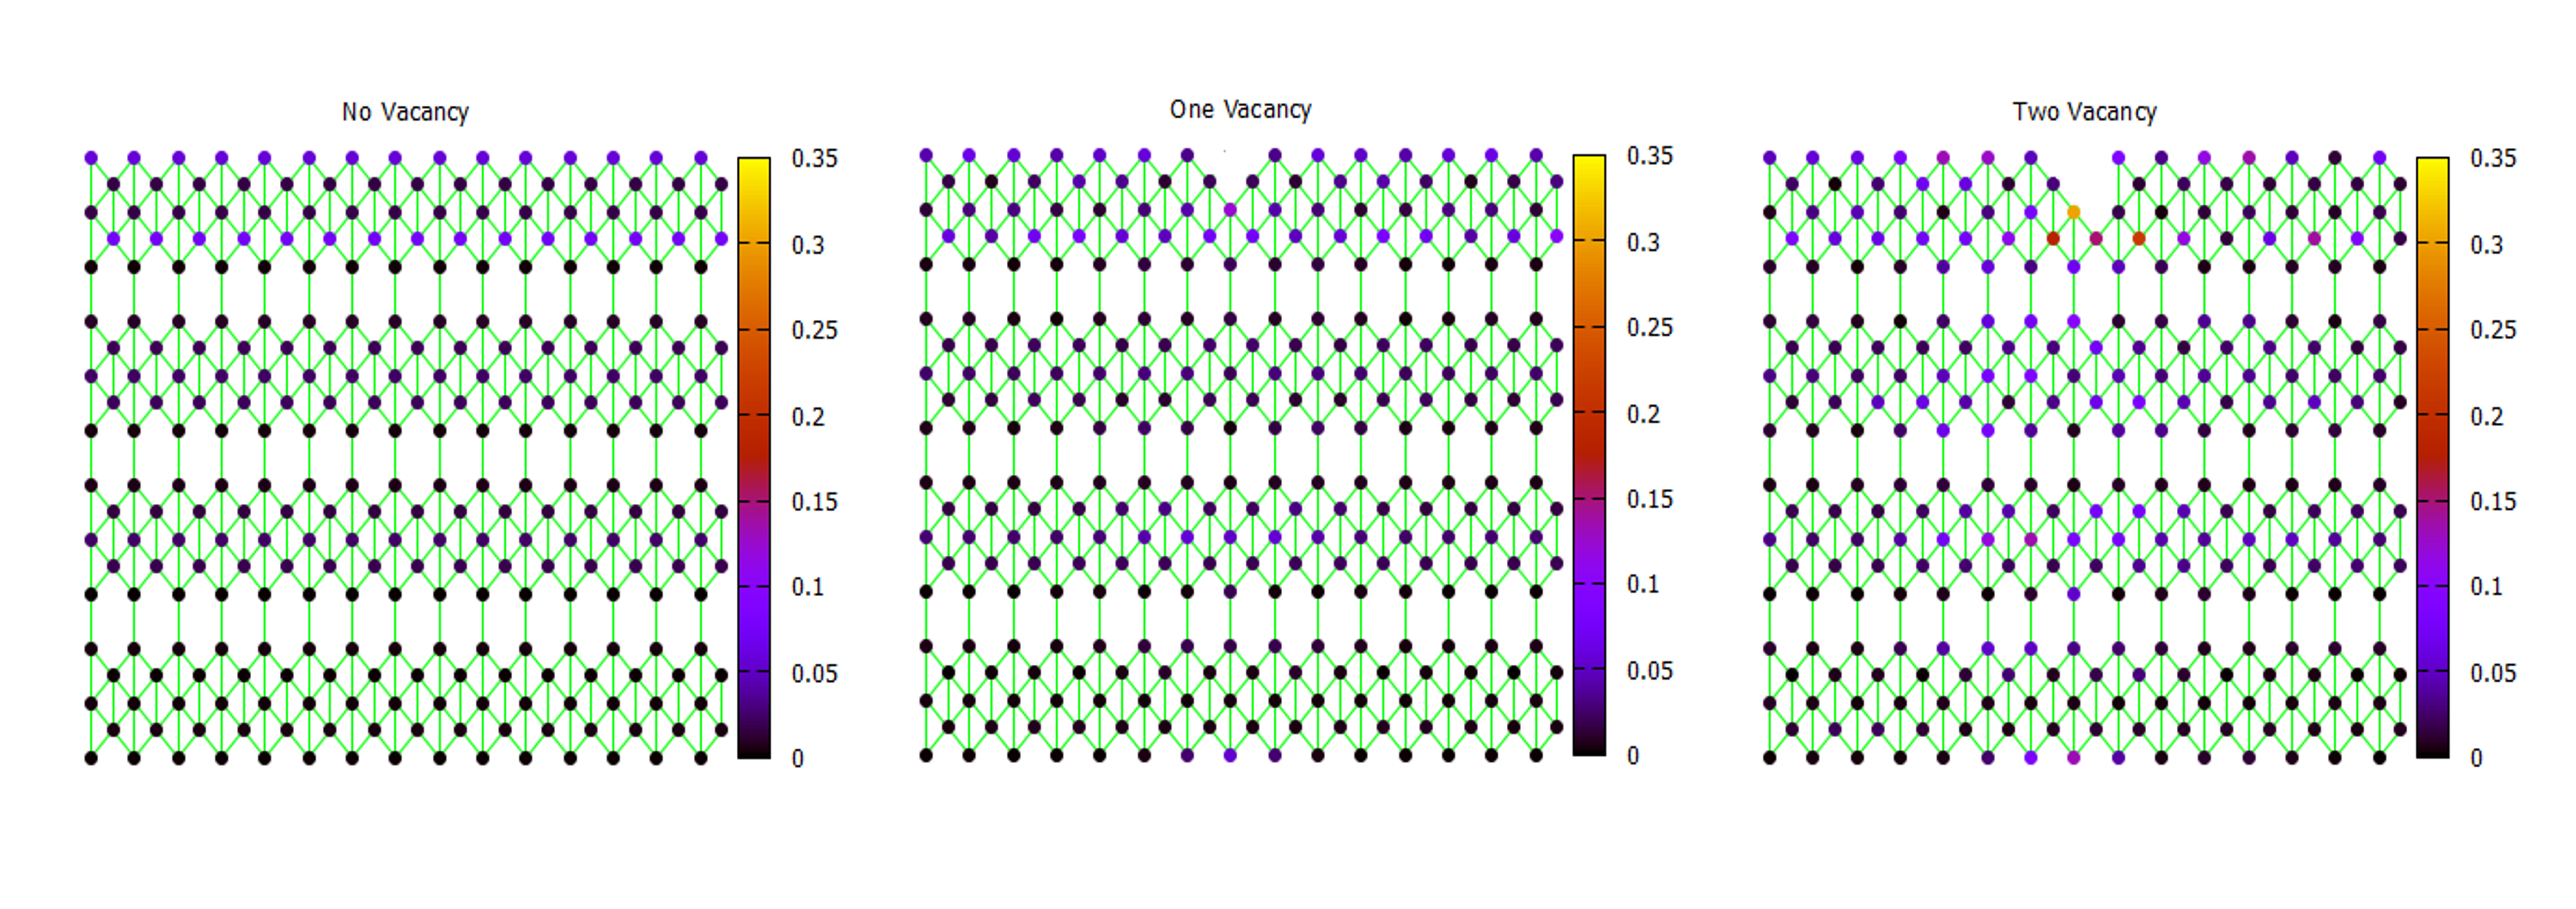
\includegraphics[width=1\linewidth]{./figures/Slide4.PNG}
    \caption{در انرژی مربوط به اوج \lr{LDOS} در نزدیکی انرژی فرمی، چگالی الکترونی فضایی حالت‌ها در کل محل نانوروبان بوروفن زیگزاگ با یک محل خالی در لبه بالایی خالی، یک جای خالی و دو جای خالی در وسط رسم شد. از نانو روبان}
    \label{zigVSLDOS}
\end{figure}
\begin{figure}[!ht]
\centering
% GNUPLOT: LaTeX picture with Postscript
\begingroup
  % Encoding inside the plot.  In the header of your document, this encoding
  % should to defined, e.g., by using
  % \usepackage[cp1252,<other encodings>]{inputenc}
  % \inputencoding{cp1252}%
  \makeatletter
  \providecommand\color[2][]{%
    \GenericError{(gnuplot) \space\space\space\@spaces}{%
      Package color not loaded in conjunction with
      terminal option `colourtext'%
    }{See the gnuplot documentation for explanation.%
    }{Either use 'blacktext' in gnuplot or load the package
      color.sty in LaTeX.}%
    \renewcommand\color[2][]{}%
  }%
  \providecommand\includegraphics[2][]{%
    \GenericError{(gnuplot) \space\space\space\@spaces}{%
      Package graphicx or graphics not loaded%
    }{See the gnuplot documentation for explanation.%
    }{The gnuplot epslatex terminal needs graphicx.sty or graphics.sty.}%
    \renewcommand\includegraphics[2][]{}%
  }%
  \providecommand\rotatebox[2]{#2}%
  \@ifundefined{ifGPcolor}{%
    \newif\ifGPcolor
    \GPcolorfalse
  }{}%
  \@ifundefined{ifGPblacktext}{%
    \newif\ifGPblacktext
    \GPblacktexttrue
  }{}%
  % define a \g@addto@macro without @ in the name:
  \let\gplgaddtomacro\g@addto@macro
  % define empty templates for all commands taking text:
  \gdef\gplbacktext{}%
  \gdef\gplfronttext{}%
  \makeatother
  \ifGPblacktext
    % no textcolor at all
    \def\colorrgb#1{}%
    \def\colorgray#1{}%
  \else
    % gray or color?
    \ifGPcolor
      \def\colorrgb#1{\color[rgb]{#1}}%
      \def\colorgray#1{\color[gray]{#1}}%
      \expandafter\def\csname LTw\endcsname{\color{white}}%
      \expandafter\def\csname LTb\endcsname{\color{black}}%
      \expandafter\def\csname LTa\endcsname{\color{black}}%
      \expandafter\def\csname LT0\endcsname{\color[rgb]{1,0,0}}%
      \expandafter\def\csname LT1\endcsname{\color[rgb]{0,1,0}}%
      \expandafter\def\csname LT2\endcsname{\color[rgb]{0,0,1}}%
      \expandafter\def\csname LT3\endcsname{\color[rgb]{1,0,1}}%
      \expandafter\def\csname LT4\endcsname{\color[rgb]{0,1,1}}%
      \expandafter\def\csname LT5\endcsname{\color[rgb]{1,1,0}}%
      \expandafter\def\csname LT6\endcsname{\color[rgb]{0,0,0}}%
      \expandafter\def\csname LT7\endcsname{\color[rgb]{1,0.3,0}}%
      \expandafter\def\csname LT8\endcsname{\color[rgb]{0.5,0.5,0.5}}%
    \else
      % gray
      \def\colorrgb#1{\color{black}}%
      \def\colorgray#1{\color[gray]{#1}}%
      \expandafter\def\csname LTw\endcsname{\color{white}}%
      \expandafter\def\csname LTb\endcsname{\color{black}}%
      \expandafter\def\csname LTa\endcsname{\color{black}}%
      \expandafter\def\csname LT0\endcsname{\color{black}}%
      \expandafter\def\csname LT1\endcsname{\color{black}}%
      \expandafter\def\csname LT2\endcsname{\color{black}}%
      \expandafter\def\csname LT3\endcsname{\color{black}}%
      \expandafter\def\csname LT4\endcsname{\color{black}}%
      \expandafter\def\csname LT5\endcsname{\color{black}}%
      \expandafter\def\csname LT6\endcsname{\color{black}}%
      \expandafter\def\csname LT7\endcsname{\color{black}}%
      \expandafter\def\csname LT8\endcsname{\color{black}}%
    \fi
  \fi
    \setlength{\unitlength}{0.0500bp}%
    \ifx\gptboxheight\undefined%
      \newlength{\gptboxheight}%
      \newlength{\gptboxwidth}%
      \newsavebox{\gptboxtext}%
    \fi%
    \setlength{\fboxrule}{0.5pt}%
    \setlength{\fboxsep}{1pt}%
\begin{picture}(5040.00,4320.00)%
    \gplgaddtomacro\gplbacktext{%
      \csname LTb\endcsname%%
      \put(550,704){\makebox(0,0)[r]{\strut{}$0$}}%
      \put(550,1128){\makebox(0,0)[r]{\strut{}$1$}}%
      \put(550,1553){\makebox(0,0)[r]{\strut{}$2$}}%
      \put(550,1977){\makebox(0,0)[r]{\strut{}$3$}}%
      \put(550,2402){\makebox(0,0)[r]{\strut{}$4$}}%
      \put(550,2826){\makebox(0,0)[r]{\strut{}$5$}}%
      \put(550,3250){\makebox(0,0)[r]{\strut{}$6$}}%
      \put(550,3675){\makebox(0,0)[r]{\strut{}$7$}}%
      \put(550,4099){\makebox(0,0)[r]{\strut{}$8$}}%
      \put(682,484){\makebox(0,0){\strut{}$-2$}}%
      \put(1177,484){\makebox(0,0){\strut{}$-1.5$}}%
      \put(1672,484){\makebox(0,0){\strut{}$-1$}}%
      \put(2167,484){\makebox(0,0){\strut{}$-0.5$}}%
      \put(2663,484){\makebox(0,0){\strut{}$0$}}%
      \put(3158,484){\makebox(0,0){\strut{}$0.5$}}%
      \put(3653,484){\makebox(0,0){\strut{}$1$}}%
      \put(4148,484){\makebox(0,0){\strut{}$1.5$}}%
      \put(4643,484){\makebox(0,0){\strut{}$2$}}%
    }%
    \gplgaddtomacro\gplfronttext{%
      \csname LTb\endcsname%%
      \put(198,2401){\rotatebox{-270}{\makebox(0,0){\strut{}$G/G_0$}}}%
      \put(2662,154){\makebox(0,0){\strut{}Energy(eV)}}%
      \csname LTb\endcsname%%
      \put(3656,3926){\makebox(0,0)[r]{\strut{}pristine ZBNR}}%
      \csname LTb\endcsname%%
      \put(3656,3706){\makebox(0,0)[r]{\strut{}V=0.25 eV}}%
      \csname LTb\endcsname%%
      \put(3656,3486){\makebox(0,0)[r]{\strut{}V=0.5 eV}}%
      \csname LTb\endcsname%%
      \put(3656,3266){\makebox(0,0)[r]{\strut{}V=2 eV}}%
    }%
    \gplbacktext
    \put(0,0){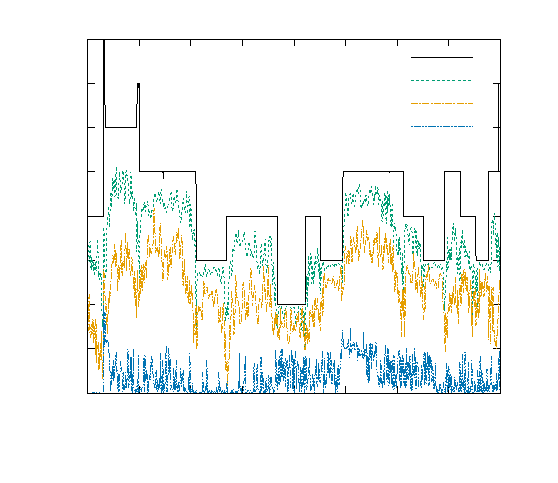
\includegraphics[width={253.00bp},height={217.00bp}]{zigzagdisorder}}%
    \gplfronttext
  \end{picture}%
\endgroup

\caption{رسانایی در مقابل انرژی برای نوارهای زیگزاگی با عرض \lr{\AA} 10.24 و با بی نظمی در هر دو لبه به طول \lr{\AA} 876.68 توزیع شده است
با یک اختلال نسبتا ضعیف $V_d=2\;eV$، \lr{BNR} های زیگزاگی از فلز به نیمه هادی تبدیل می شوند.}
\label{zigzagdisorder}
\end{figure}
توزیع چگالی حالت‌ها در همه مکان‌های نانوروبان به انرژی بستگی دارد. توزیع چگالی حالت‌ها حول $E=-0.034$ ترسیم شده است در شکل\ref{zigCSLDOS}. شکل\ref{zigCSLDOS} نشان می دهد که در حالی که هیچ پراکنده ای روی نانوروبان وجود ندارد، توزیع چگالی حالت‌ها تقریباً در همه مکان‌ها برابر است. با قرار دادن پراکنده در لبه بالایی سوپرسل میانی نانوروبان معادل شکل\ref{fig:borophene}، توزیع چگالی حالت‌ها در اطراف ابرسلول میانی افزایش می یابد. با افزایش قدرت پراکندگی، چگالی حالات در اطراف ابرسلول مرکزی افزایش می یابد. با افزایش قدرت پراکنده، توزیع چگالی حالت‌ها به سمت نزدیکترین محل به پراکنده مشهود است. در شکل\ref{armscatter}(a) و شکل \ref{armscatter}(b)،رسانایی و \lr{LDOS} به ترتیب برای \lr{ABNR}ها با عرض \lr{\AA} 10.24 رسم شده است. ناخالصی در لبه بالایی سوپرسل میانی نانوروبان قرار دارد. در هر دو \lr{BNR} آرمچیر و زیگزاگ، ناخالصی های ضعیف نمی توانند بر رسانایی تأثیر بگذارند. با این حال، با افزایش قدرت پتانسیل ناخالصی ها، شیب رسانایی در اطراف انرژی فرمی همزمان با پیک \lr{LDOS} در محل مجاور ناخالصی ایجاد می شود. بنابراین حالت های شبه موضعی را می توان در ناخالصی های قوی مشاهده کرد. در \lr{ZBNR} ها، فرورفتگی های رسانایی، در نتیجه ناخالصی لبه، به وضوح در لبه نوار مشاهده می شود، و عرض شیب‌ها زمانی که قدرت پتانسیل نقص مشاهده می شود، قابل توجه می شود. بیشتر از $2 eV$ با این حال، در \lr{ABNR} ها، یک شیب رسانایی در اطراف انرژی فرمی ظاهر می شود، جایی که یک پیک معادل، مرتبط با حالت های شبه موضعی را می توان در LDOS مشاهده کرد، زمانی که نقص قدرت بالقوه $5 eV$ باشد. شکل \ref{armCSLDOS} افزایش چگالی حالت‌ها را در اطراف سوپرسل میانی نانوروبان با لبه های آرمچیر با انرژی 0.19 eV نشان می دهد. علاوه بر این، نشان می دهد که یک پراکنده روی لبه بوروفن با لبه آرمچیر دارای تأثیر بیشتری نسبت به یک پراکنده روی لبه بوروفن با لبه زیگزاگ است. بنابراین این موضوع مقایسه رسانایی و \lr{LDOS} در شکل \ref{zigscatter} و \ref{armscatter} را تایید می کند که اثر پراکندگی بر روی رسانایی و نمودار \lr{LDOS} بوروفن با لبه آرمچیر آرمچیر قابل توجه تر است. در شکل \ref{armvacancy}، رسانایی و \lr{LDOS} مربوطه برای \lr{ABNR}ها با عرض \lr{\AA} 10.24 (4 سلول واحد در سوپرسل) در دو حالت خالی، یک یا دو اتم خالی ترسیم شده است. تأثیر جای خالی لبه تک اتمی و جای خالی لبه دو اتمی بر رسانایی \lr{ABNR} ها کاملاً متفاوت است. در حالت اول، فرورفتگیهای رسانایی در لبههای نوارها ظاهر میشوند، که متفاوت از تکینگیهای \lr{Van-Hoff} سیستم بکر است، بنابراین شواهدی مبنی بر وجود شبه ذرات در آن انرژی وجود دارد. قبلاً دیده شده است که یک شبکه لانه زنبوری پنهان در ساختار شبکه $\beta_{12}$ وجود دارد و متعاقباً مشابه گرافن، ممکن است دو زیرشبکه تعریف شود. در نتیجه، شیب رسانایی برجسته در دومی، که با یک قله بزرگ در \lr{LDOS} در انرژی فرمی همراه است، از شکستن تقارن زیرشبکه نشات میگیرد. همانطور که قبلا ذکر کردیم، در حالی که قدرت پراکندگی را تا بی نهایت افزایش می دهیم، به نانوروبان با یک جای خالی در لبه می رسیم. بنابراین، چگالی حالتها در اطراف سوپرسل میانی دارای بیشترین غلظت و تقریباً مقدار قابل توجهی \lr{LDOS} است که در نزدیکترین مکان به جای خالی قرار میگیرد. شکست تقارن انتقالی در حضور یک جای خالی در نانوروبان با لبه آرمچیر در شکل \ref{zigVSLDOS} مشاهده شده است و نتایج قبلی ذکر شده در شکل \ref{zigvacancy} را تایید می کند. \lr{ZBNR}های با جای خالی لبهای رفتاری مشابه با جای خالی لبههای نانوروبانهای گرافن آرمچیر راحتی دارند، زیرا فرورفتگیهای رسانایی در لبههای نوارهای مربوط به قلههای \lr{LDOS} رخ میدهد تا حالتهای شبه موضعی ممکن است نتیجهگیری شود. با این حال، در مورد جاهای خالی لبه دو اتمی در \lr{ZBNR}، یک شیب رسانایی بزرگ با یک \lr{LDOS} بزرگ معادل در انرژی فرمی دیده میشود، مانند مورد \lr{ABNR}، که کاملاً با \lr{GNRs} متناقض است.

این را می توان با شکستن تقارن توضیح داد. زیرشبکه به دلیل وجود اتم میانی در سلول واحد در لبه. همچنین، در بوروفن با لبه زیگزاگ (شکل\ref{zigVSLDOS})، مانند \lr{ABNR}ها، حد نهایی LDOS در نزدیکترین محل پراکنده نشان داده شده است و می توان مشاهده کرد که نتایج قبلی به دست آمده از شکل \ref{zigvacancy} را تایید می کند.
% چگالی الکترونی فضایی حالتها در کل محل نانوروبان بوروفن آرمچیر با یک مکان پراکندگی در لبه بالایی با \lr{V=0،1،2،5} در وسط نانوروبان ترسیم شده است. شکل\ref{zigvacancy}.

بورفن زیگزاگ و آرمچیر با نقص‌های منفرد و اختلالات ضعیف در لبه‌ها را در چارچوب مدل اتصال محکم با استفاده از تکنیک تابع گرین بررسی کرده‌ایم. رسانایی نانوروبانهای بوروفن بکر رفتار گام به گام را نشان میدهد و تعداد کانالهای رسانایی در انرژی فرمی به عرض بوروفن بستگی دارد، به دلیل وجود اتم مرکزی در سلول واحد بوروفن، در تضاد واضح با مورد گرافن. ابتدا دو نوع نقص لبه را معرفی میکنیم، یعنی نقصهای منفرد شامل تک پراکندگی و تک خالی و اختلال ضعیف. نانوروبانهای بوروفن زیگزاگ همگی رفتار فلزی از خود نشان میدهند، در حالی که \lr{BNR}های آرمچیر راحتی بسته به عرض، رفتار فلزی یا نیمرسانا را نشان میدهند. مشخص شده است که عیوب منفرد لبهای باعث حالتهای شبه موضعی میشوند و بنابراین افت رسانایی ظاهر میشوند. بنابراین، این نتایج ممکن است وجود شبکه لانه زنبوری پنهان را در داخل یک $\beta_{12}$-بوروفن با وجود ساختار شبکه مستطیلی آن تأیید کند. علاوه بر این، جای خالی یک اتمی و دو اتمی بر ترابرد الکترون‌ها به طور قابل توجهی نسبت به مورد قبلی از طریق تشکیل حالت های شبه موضعی و افت رسانایی تأثیر می گذارد. در \lr{BNR} های آرمچیر، جای خالی یک اتمی باعث شکسته شدن تقارن زیرشبکه می شود و بنابراین رسانایی را بیشتر از جای خالی دو اتمی تحت تاثیر قرار می دهد، در حالی که در \lr{BNR} های زیگزاگ، جای خالی دو اتمی تقارن زیرشبکه را شکسته و ترابرد را بیش از جای خالی یک اتمی تحت تاثیر قرار می دهد. توزیع تصادفی پراکندگی ضعیف روی لبههای \lr{BNR} باعث میشود که جایگزیدهسازی اندرسون اتفاق بیفتد، که منجر به ترابرد فلز به نیمهرسانا میشود. در \lr{BNR} ها، طول جایگزیده سازی اندرسون برای استحکام پتانسیل پایین بسیار طولانی است که با افزایش قدرت پتانسیل کاهش می یابد. با افزایش طول نانوروبان، رسانایی تا حد زیادی کاهش می یابد. در \lr{BNR} های آرمچیر راحتی، پتانسیل های استحکام ضعیف باعث طول کوتاه تری نسبت به جایگزیده سازی اندرسون در مقایسه با \lr{BNR} های زیگزاگ می شود. علاوه بر این، طول جایگزیده سازی به عرض \lr{BNR} ها بستگی دارد به طوری که با افزایش عرض \lr{BNR} ها، طول جایگزیده سازی نیز افزایش می یابد.

\subsection{پراکندگی اندرسون}
 در اینجا باید به کلیت پراکندگی اندرسون بپردازیم. و شقوق مختلف آنرا بیان کینم و در اخر نتایج خود رادر مورد بورفین اعلام کنیم.
% a† i (ai ) عملگرهای ایجاد الکترون (نابودی) در الکترون π در جایگاه i هستند، εi انرژی در محل در i-site و tij انرژی پرش نزدیکترین همسایه است. سرعت فرمی در جهات مختلف با انبساط همیلتونی در فضای فوریه حول یک نقطه شبکه متقابل به دست می آید، به طوری که انرژی های جهشی مختلف در بوروفن منجر به سرعت های متفاوتی در آن می شود. شایان ذکر است که به منظور شبیه سازی وجود ناخالصی ها، اصطلاحاً پراکندگی ضعیف، عبارت دیگری حاوی انرژی در محل ωi به هامیلتونین اضافه می شود. از آنجایی که مدل وارونگی غیر متقارن با آزمایشات [26] سازگار است، ما از ضرایب مربوطه در هامیلتونی استفاده می کنیم. یک لایه $\beta_{12}$ را به سه قسمت تقسیم می کنیم. نانوروبان، به عنوان بخش مرکزی سیستم، ناحیه پراکنده ای است که توسط دو سرب نیمه نامتناهی احاطه شده است. ما نانوروبان را به عنوان یک سیم 1 بعدی با دو نوع لبه در نظر می گیریم. بسته به محل سرنخ ها، با سیم 1 بعدی ایجاد شده از نانوروبان های بوروفن زیگزاگ (ZBNRs) یا نانوروبان های بوروفن \lr{Armchair (ABNRs)} مواجه می شویم. به منظور بررسی رسانایی $\beta_{12}$، از روش لوپز سانچو برای محاسبه تابع گرین سطح [56] به صورت زیر استفاده می شود:
% که در آن Hl,l همیلتونین ابرسلولهای BNRها است و Hl,l+1 ماتریس برهمکنش بین BNRهای مجاور است. ، ̃ ماتریس های انتقالی هستند که توسط عناصر ماتریس همیلتونی با اتصال محکم با استفاده از روش بازگشتی به دست می آیند [48].

\begin{figure}[!ht]
    \centering
      % GNUPLOT: LaTeX picture with Postscript
\begingroup
  % Encoding inside the plot.  In the header of your document, this encoding
  % should to defined, e.g., by using
  % \usepackage[cp1252,<other encodings>]{inputenc}
  % \inputencoding{cp1252}%
  \makeatletter
  \providecommand\color[2][]{%
    \GenericError{(gnuplot) \space\space\space\@spaces}{%
      Package color not loaded in conjunction with
      terminal option `colourtext'%
    }{See the gnuplot documentation for explanation.%
    }{Either use 'blacktext' in gnuplot or load the package
      color.sty in LaTeX.}%
    \renewcommand\color[2][]{}%
  }%
  \providecommand\includegraphics[2][]{%
    \GenericError{(gnuplot) \space\space\space\@spaces}{%
      Package graphicx or graphics not loaded%
    }{See the gnuplot documentation for explanation.%
    }{The gnuplot epslatex terminal needs graphicx.sty or graphics.sty.}%
    \renewcommand\includegraphics[2][]{}%
  }%
  \providecommand\rotatebox[2]{#2}%
  \@ifundefined{ifGPcolor}{%
    \newif\ifGPcolor
    \GPcolorfalse
  }{}%
  \@ifundefined{ifGPblacktext}{%
    \newif\ifGPblacktext
    \GPblacktexttrue
  }{}%
  % define a \g@addto@macro without @ in the name:
  \let\gplgaddtomacro\g@addto@macro
  % define empty templates for all commands taking text:
  \gdef\gplbacktext{}%
  \gdef\gplfronttext{}%
  \makeatother
  \ifGPblacktext
    % no textcolor at all
    \def\colorrgb#1{}%
    \def\colorgray#1{}%
  \else
    % gray or color?
    \ifGPcolor
      \def\colorrgb#1{\color[rgb]{#1}}%
      \def\colorgray#1{\color[gray]{#1}}%
      \expandafter\def\csname LTw\endcsname{\color{white}}%
      \expandafter\def\csname LTb\endcsname{\color{black}}%
      \expandafter\def\csname LTa\endcsname{\color{black}}%
      \expandafter\def\csname LT0\endcsname{\color[rgb]{1,0,0}}%
      \expandafter\def\csname LT1\endcsname{\color[rgb]{0,1,0}}%
      \expandafter\def\csname LT2\endcsname{\color[rgb]{0,0,1}}%
      \expandafter\def\csname LT3\endcsname{\color[rgb]{1,0,1}}%
      \expandafter\def\csname LT4\endcsname{\color[rgb]{0,1,1}}%
      \expandafter\def\csname LT5\endcsname{\color[rgb]{1,1,0}}%
      \expandafter\def\csname LT6\endcsname{\color[rgb]{0,0,0}}%
      \expandafter\def\csname LT7\endcsname{\color[rgb]{1,0.3,0}}%
      \expandafter\def\csname LT8\endcsname{\color[rgb]{0.5,0.5,0.5}}%
    \else
      % gray
      \def\colorrgb#1{\color{black}}%
      \def\colorgray#1{\color[gray]{#1}}%
      \expandafter\def\csname LTw\endcsname{\color{white}}%
      \expandafter\def\csname LTb\endcsname{\color{black}}%
      \expandafter\def\csname LTa\endcsname{\color{black}}%
      \expandafter\def\csname LT0\endcsname{\color{black}}%
      \expandafter\def\csname LT1\endcsname{\color{black}}%
      \expandafter\def\csname LT2\endcsname{\color{black}}%
      \expandafter\def\csname LT3\endcsname{\color{black}}%
      \expandafter\def\csname LT4\endcsname{\color{black}}%
      \expandafter\def\csname LT5\endcsname{\color{black}}%
      \expandafter\def\csname LT6\endcsname{\color{black}}%
      \expandafter\def\csname LT7\endcsname{\color{black}}%
      \expandafter\def\csname LT8\endcsname{\color{black}}%
    \fi
  \fi
    \setlength{\unitlength}{0.0500bp}%
    \ifx\gptboxheight\undefined%
      \newlength{\gptboxheight}%
      \newlength{\gptboxwidth}%
      \newsavebox{\gptboxtext}%
    \fi%
    \setlength{\fboxrule}{0.5pt}%
    \setlength{\fboxsep}{1pt}%
\begin{picture}(5040.00,4320.00)%
    \gplgaddtomacro\gplbacktext{%
      \csname LTb\endcsname%%
      \put(550,704){\makebox(0,0)[r]{\strut{}$0$}}%
      \put(550,1270){\makebox(0,0)[r]{\strut{}$1$}}%
      \put(550,1836){\makebox(0,0)[r]{\strut{}$2$}}%
      \put(550,2402){\makebox(0,0)[r]{\strut{}$3$}}%
      \put(550,2967){\makebox(0,0)[r]{\strut{}$4$}}%
      \put(550,3533){\makebox(0,0)[r]{\strut{}$5$}}%
      \put(550,4099){\makebox(0,0)[r]{\strut{}$6$}}%
      \put(682,484){\makebox(0,0){\strut{}$-2$}}%
      \put(1342,484){\makebox(0,0){\strut{}$-1.5$}}%
      \put(2002,484){\makebox(0,0){\strut{}$-1$}}%
      \put(2662,484){\makebox(0,0){\strut{}$-0.5$}}%
      \put(3323,484){\makebox(0,0){\strut{}$0$}}%
      \put(3983,484){\makebox(0,0){\strut{}$0.5$}}%
      \put(4643,484){\makebox(0,0){\strut{}$1$}}%
    }%
    \gplgaddtomacro\gplfronttext{%
      \csname LTb\endcsname%%
      \put(198,2401){\rotatebox{-270}{\makebox(0,0){\strut{}$G/G_0$}}}%
      \put(2662,154){\makebox(0,0){\strut{}Energy(eV)}}%
      \csname LTb\endcsname%%
      \put(3656,3926){\makebox(0,0)[r]{\strut{}pristine ABNR}}%
      \csname LTb\endcsname%%
      \put(3656,3706){\makebox(0,0)[r]{\strut{}V=0.25 eV}}%
      \csname LTb\endcsname%%
      \put(3656,3486){\makebox(0,0)[r]{\strut{}V=0.5 eV}}%
      \csname LTb\endcsname%%
      \put(3656,3266){\makebox(0,0)[r]{\strut{}V=1 eV}}%
    }%
    \gplbacktext
    \put(0,0){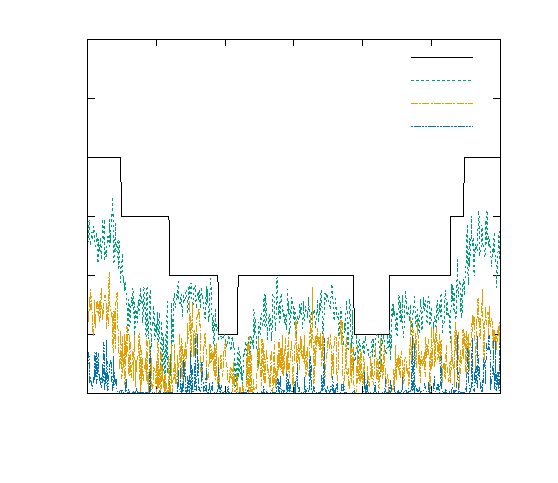
\includegraphics[width={253.00bp},height={217.00bp}]{armdisorder}}%
    \gplfronttext
  \end{picture}%
\endgroup

      \caption{رسانایی در مقابل انرژی برای نوارهای آرمچیر با عرض $18.59$\AA و با بی نظمی توزیع شده در هر دو لبه در طول $758.81$\AA با اختلال نسبتا ضعیف $V_d=1\;eV$، BNRهای آرمچیر از فلز به نیمه هادی تبدیل می شوند.}
      \label{armdisorder}
    \end{figure}
    
    \begin{figure*}[!ht]
      \centering
      % GNUPLOT: LaTeX picture with Postscript
\begingroup
  % Encoding inside the plot.  In the header of your document, this encoding
  % should to defined, e.g., by using
  % \usepackage[cp1252,<other encodings>]{inputenc}
  % \inputencoding{cp1252}%
  \makeatletter
  \providecommand\color[2][]{%
    \GenericError{(gnuplot) \space\space\space\@spaces}{%
      Package color not loaded in conjunction with
      terminal option `colourtext'%
    }{See the gnuplot documentation for explanation.%
    }{Either use 'blacktext' in gnuplot or load the package
      color.sty in LaTeX.}%
    \renewcommand\color[2][]{}%
  }%
  \providecommand\includegraphics[2][]{%
    \GenericError{(gnuplot) \space\space\space\@spaces}{%
      Package graphicx or graphics not loaded%
    }{See the gnuplot documentation for explanation.%
    }{The gnuplot epslatex terminal needs graphicx.sty or graphics.sty.}%
    \renewcommand\includegraphics[2][]{}%
  }%
  \providecommand\rotatebox[2]{#2}%
  \@ifundefined{ifGPcolor}{%
    \newif\ifGPcolor
    \GPcolorfalse
  }{}%
  \@ifundefined{ifGPblacktext}{%
    \newif\ifGPblacktext
    \GPblacktexttrue
  }{}%
  % define a \g@addto@macro without @ in the name:
  \let\gplgaddtomacro\g@addto@macro
  % define empty templates for all commands taking text:
  \gdef\gplbacktext{}%
  \gdef\gplfronttext{}%
  \makeatother
  \ifGPblacktext
    % no textcolor at all
    \def\colorrgb#1{}%
    \def\colorgray#1{}%
  \else
    % gray or color?
    \ifGPcolor
      \def\colorrgb#1{\color[rgb]{#1}}%
      \def\colorgray#1{\color[gray]{#1}}%
      \expandafter\def\csname LTw\endcsname{\color{white}}%
      \expandafter\def\csname LTb\endcsname{\color{black}}%
      \expandafter\def\csname LTa\endcsname{\color{black}}%
      \expandafter\def\csname LT0\endcsname{\color[rgb]{1,0,0}}%
      \expandafter\def\csname LT1\endcsname{\color[rgb]{0,1,0}}%
      \expandafter\def\csname LT2\endcsname{\color[rgb]{0,0,1}}%
      \expandafter\def\csname LT3\endcsname{\color[rgb]{1,0,1}}%
      \expandafter\def\csname LT4\endcsname{\color[rgb]{0,1,1}}%
      \expandafter\def\csname LT5\endcsname{\color[rgb]{1,1,0}}%
      \expandafter\def\csname LT6\endcsname{\color[rgb]{0,0,0}}%
      \expandafter\def\csname LT7\endcsname{\color[rgb]{1,0.3,0}}%
      \expandafter\def\csname LT8\endcsname{\color[rgb]{0.5,0.5,0.5}}%
    \else
      % gray
      \def\colorrgb#1{\color{black}}%
      \def\colorgray#1{\color[gray]{#1}}%
      \expandafter\def\csname LTw\endcsname{\color{white}}%
      \expandafter\def\csname LTb\endcsname{\color{black}}%
      \expandafter\def\csname LTa\endcsname{\color{black}}%
      \expandafter\def\csname LT0\endcsname{\color{black}}%
      \expandafter\def\csname LT1\endcsname{\color{black}}%
      \expandafter\def\csname LT2\endcsname{\color{black}}%
      \expandafter\def\csname LT3\endcsname{\color{black}}%
      \expandafter\def\csname LT4\endcsname{\color{black}}%
      \expandafter\def\csname LT5\endcsname{\color{black}}%
      \expandafter\def\csname LT6\endcsname{\color{black}}%
      \expandafter\def\csname LT7\endcsname{\color{black}}%
      \expandafter\def\csname LT8\endcsname{\color{black}}%
    \fi
  \fi
    \setlength{\unitlength}{0.0500bp}%
    \ifx\gptboxheight\undefined%
      \newlength{\gptboxheight}%
      \newlength{\gptboxwidth}%
      \newsavebox{\gptboxtext}%
    \fi%
    \setlength{\fboxrule}{0.5pt}%
    \setlength{\fboxsep}{1pt}%
\begin{picture}(7200.00,5040.00)%
    \gplgaddtomacro\gplbacktext{%
      \csname LTb\endcsname%%
      \put(814,704){\makebox(0,0)[r]{\strut{}$0$}}%
      \put(814,1161){\makebox(0,0)[r]{\strut{}$0.5$}}%
      \put(814,1618){\makebox(0,0)[r]{\strut{}$1$}}%
      \put(814,2076){\makebox(0,0)[r]{\strut{}$1.5$}}%
      \put(814,2533){\makebox(0,0)[r]{\strut{}$2$}}%
      \put(814,2990){\makebox(0,0)[r]{\strut{}$2.5$}}%
      \put(814,3447){\makebox(0,0)[r]{\strut{}$3$}}%
      \put(814,3905){\makebox(0,0)[r]{\strut{}$3.5$}}%
      \put(814,4362){\makebox(0,0)[r]{\strut{}$4$}}%
      \put(814,4819){\makebox(0,0)[r]{\strut{}$4.5$}}%
      \put(946,484){\makebox(0,0){\strut{}$0$}}%
      \put(1197,484){\makebox(0,0){\strut{}$2$}}%
      \put(1448,484){\makebox(0,0){\strut{}$4$}}%
      \put(1698,484){\makebox(0,0){\strut{}$6$}}%
      \put(1949,484){\makebox(0,0){\strut{}$8$}}%
      \put(2200,484){\makebox(0,0){\strut{}$10$}}%
      \put(2451,484){\makebox(0,0){\strut{}$12$}}%
      \put(2701,484){\makebox(0,0){\strut{}$14$}}%
      \put(2952,484){\makebox(0,0){\strut{}$16$}}%
      \put(3203,484){\makebox(0,0){\strut{}$18$}}%
      \put(1172,4613){\makebox(0,0)[l]{\strut{}(a)}}%
    }%
    \gplgaddtomacro\gplfronttext{%
      \csname LTb\endcsname%%
      \put(198,2761){\rotatebox{-270}{\makebox(0,0){\strut{}$G/G_0$}}}%
      \put(2074,154){\makebox(0,0){\strut{}Length(nm)$*10^{1}$}}%
      \csname LTb\endcsname%%
      \put(2216,4646){\makebox(0,0)[r]{\strut{}W=4}}%
      \csname LTb\endcsname%%
      \put(2216,4426){\makebox(0,0)[r]{\strut{}W=6}}%
      \csname LTb\endcsname%%
      \put(2216,4206){\makebox(0,0)[r]{\strut{}W=8}}%
    }%
    \gplgaddtomacro\gplbacktext{%
      \csname LTb\endcsname%%
      \put(4414,704){\makebox(0,0)[r]{\strut{}$0$}}%
      \put(4414,1078){\makebox(0,0)[r]{\strut{}$0.5$}}%
      \put(4414,1452){\makebox(0,0)[r]{\strut{}$1$}}%
      \put(4414,1826){\makebox(0,0)[r]{\strut{}$1.5$}}%
      \put(4414,2200){\makebox(0,0)[r]{\strut{}$2$}}%
      \put(4414,2574){\makebox(0,0)[r]{\strut{}$2.5$}}%
      \put(4414,2949){\makebox(0,0)[r]{\strut{}$3$}}%
      \put(4414,3323){\makebox(0,0)[r]{\strut{}$3.5$}}%
      \put(4414,3697){\makebox(0,0)[r]{\strut{}$4$}}%
      \put(4414,4071){\makebox(0,0)[r]{\strut{}$4.5$}}%
      \put(4414,4445){\makebox(0,0)[r]{\strut{}$5$}}%
      \put(4414,4819){\makebox(0,0)[r]{\strut{}$5.5$}}%
      \put(4546,484){\makebox(0,0){\strut{}$0$}}%
      \put(4997,484){\makebox(0,0){\strut{}$1$}}%
      \put(5449,484){\makebox(0,0){\strut{}$2$}}%
      \put(5900,484){\makebox(0,0){\strut{}$3$}}%
      \put(6352,484){\makebox(0,0){\strut{}$4$}}%
      \put(6803,484){\makebox(0,0){\strut{}$5$}}%
      \put(4772,4613){\makebox(0,0)[l]{\strut{}(b)}}%
    }%
    \gplgaddtomacro\gplfronttext{%
      \csname LTb\endcsname%%
      \put(3798,2761){\rotatebox{-270}{\makebox(0,0){\strut{}$G/G_0$}}}%
      \put(5674,154){\makebox(0,0){\strut{}$V_d(eV)$}}%
      \csname LTb\endcsname%%
      \put(5816,4646){\makebox(0,0)[r]{\strut{}W=4}}%
      \csname LTb\endcsname%%
      \put(5816,4426){\makebox(0,0)[r]{\strut{}W=6}}%
      \csname LTb\endcsname%%
      \put(5816,4206){\makebox(0,0)[r]{\strut{}W=8}}%
    }%
    \gplbacktext
    \put(0,0){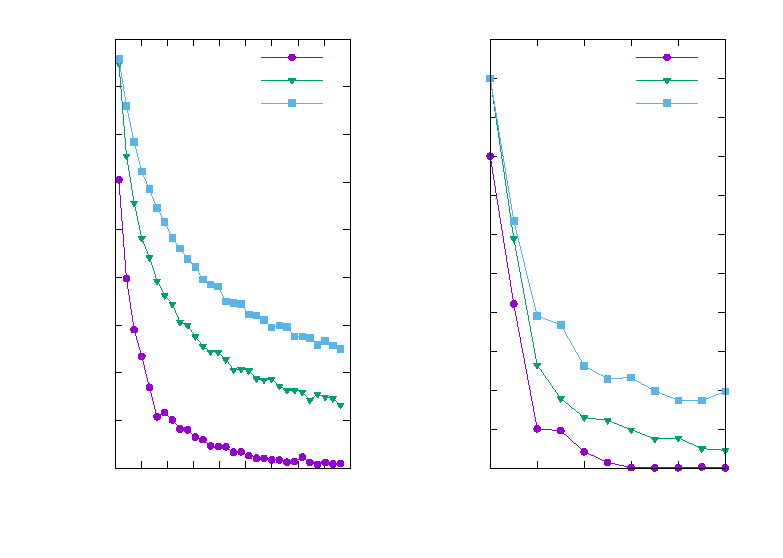
\includegraphics[width={361.00bp},height={253.00bp}]{zigzag-width-strangth}}%
    \gplfronttext
  \end{picture}%
\endgroup

      \caption{(الف) رسانایی در مقابل طول نوار با عرض های مختلف (از نظر تعداد سلول های واحد در یک ابرسلول) و قدرت بی نظمی ثابت $V_d=2\;eV$. (ب) رسانایی در برابر استحکام بی نظمی برای نوارهای زیگزاگ با بی نظمی که در هر دو لبه به طول $876.68$\AA توزیع شده است.}
      \label{zigzag-width-strangth}
    \end{figure*}  

\begin{figure*}[!ht]
    \centering
    % GNUPLOT: LaTeX picture with Postscript
\begingroup
  % Encoding inside the plot.  In the header of your document, this encoding
  % should to defined, e.g., by using
  % \usepackage[cp1252,<other encodings>]{inputenc}
  % \inputencoding{cp1252}%
  \makeatletter
  \providecommand\color[2][]{%
    \GenericError{(gnuplot) \space\space\space\@spaces}{%
      Package color not loaded in conjunction with
      terminal option `colourtext'%
    }{See the gnuplot documentation for explanation.%
    }{Either use 'blacktext' in gnuplot or load the package
      color.sty in LaTeX.}%
    \renewcommand\color[2][]{}%
  }%
  \providecommand\includegraphics[2][]{%
    \GenericError{(gnuplot) \space\space\space\@spaces}{%
      Package graphicx or graphics not loaded%
    }{See the gnuplot documentation for explanation.%
    }{The gnuplot epslatex terminal needs graphicx.sty or graphics.sty.}%
    \renewcommand\includegraphics[2][]{}%
  }%
  \providecommand\rotatebox[2]{#2}%
  \@ifundefined{ifGPcolor}{%
    \newif\ifGPcolor
    \GPcolorfalse
  }{}%
  \@ifundefined{ifGPblacktext}{%
    \newif\ifGPblacktext
    \GPblacktexttrue
  }{}%
  % define a \g@addto@macro without @ in the name:
  \let\gplgaddtomacro\g@addto@macro
  % define empty templates for all commands taking text:
  \gdef\gplbacktext{}%
  \gdef\gplfronttext{}%
  \makeatother
  \ifGPblacktext
    % no textcolor at all
    \def\colorrgb#1{}%
    \def\colorgray#1{}%
  \else
    % gray or color?
    \ifGPcolor
      \def\colorrgb#1{\color[rgb]{#1}}%
      \def\colorgray#1{\color[gray]{#1}}%
      \expandafter\def\csname LTw\endcsname{\color{white}}%
      \expandafter\def\csname LTb\endcsname{\color{black}}%
      \expandafter\def\csname LTa\endcsname{\color{black}}%
      \expandafter\def\csname LT0\endcsname{\color[rgb]{1,0,0}}%
      \expandafter\def\csname LT1\endcsname{\color[rgb]{0,1,0}}%
      \expandafter\def\csname LT2\endcsname{\color[rgb]{0,0,1}}%
      \expandafter\def\csname LT3\endcsname{\color[rgb]{1,0,1}}%
      \expandafter\def\csname LT4\endcsname{\color[rgb]{0,1,1}}%
      \expandafter\def\csname LT5\endcsname{\color[rgb]{1,1,0}}%
      \expandafter\def\csname LT6\endcsname{\color[rgb]{0,0,0}}%
      \expandafter\def\csname LT7\endcsname{\color[rgb]{1,0.3,0}}%
      \expandafter\def\csname LT8\endcsname{\color[rgb]{0.5,0.5,0.5}}%
    \else
      % gray
      \def\colorrgb#1{\color{black}}%
      \def\colorgray#1{\color[gray]{#1}}%
      \expandafter\def\csname LTw\endcsname{\color{white}}%
      \expandafter\def\csname LTb\endcsname{\color{black}}%
      \expandafter\def\csname LTa\endcsname{\color{black}}%
      \expandafter\def\csname LT0\endcsname{\color{black}}%
      \expandafter\def\csname LT1\endcsname{\color{black}}%
      \expandafter\def\csname LT2\endcsname{\color{black}}%
      \expandafter\def\csname LT3\endcsname{\color{black}}%
      \expandafter\def\csname LT4\endcsname{\color{black}}%
      \expandafter\def\csname LT5\endcsname{\color{black}}%
      \expandafter\def\csname LT6\endcsname{\color{black}}%
      \expandafter\def\csname LT7\endcsname{\color{black}}%
      \expandafter\def\csname LT8\endcsname{\color{black}}%
    \fi
  \fi
    \setlength{\unitlength}{0.0500bp}%
    \ifx\gptboxheight\undefined%
      \newlength{\gptboxheight}%
      \newlength{\gptboxwidth}%
      \newsavebox{\gptboxtext}%
    \fi%
    \setlength{\fboxrule}{0.5pt}%
    \setlength{\fboxsep}{1pt}%
\begin{picture}(7200.00,5040.00)%
    \gplgaddtomacro\gplbacktext{%
      \csname LTb\endcsname%%
      \put(814,704){\makebox(0,0)[r]{\strut{}$0$}}%
      \put(814,1390){\makebox(0,0)[r]{\strut{}$0.5$}}%
      \put(814,2076){\makebox(0,0)[r]{\strut{}$1$}}%
      \put(814,2762){\makebox(0,0)[r]{\strut{}$1.5$}}%
      \put(814,3447){\makebox(0,0)[r]{\strut{}$2$}}%
      \put(814,4133){\makebox(0,0)[r]{\strut{}$2.5$}}%
      \put(814,4819){\makebox(0,0)[r]{\strut{}$3$}}%
      \put(946,484){\makebox(0,0){\strut{}$0$}}%
      \put(1322,484){\makebox(0,0){\strut{}$5$}}%
      \put(1698,484){\makebox(0,0){\strut{}$10$}}%
      \put(2075,484){\makebox(0,0){\strut{}$15$}}%
      \put(2451,484){\makebox(0,0){\strut{}$20$}}%
      \put(2827,484){\makebox(0,0){\strut{}$25$}}%
      \put(3203,484){\makebox(0,0){\strut{}$30$}}%
      \put(1172,4613){\makebox(0,0)[l]{\strut{}(a)}}%
    }%
    \gplgaddtomacro\gplfronttext{%
      \csname LTb\endcsname%%
      \put(209,2761){\rotatebox{-270}{\makebox(0,0){\strut{}$G/G_0$}}}%
      \put(2074,154){\makebox(0,0){\strut{}Lenght(nm)$*10^{1}$}}%
      \csname LTb\endcsname%%
      \put(2216,4646){\makebox(0,0)[r]{\strut{}W=4}}%
      \csname LTb\endcsname%%
      \put(2216,4426){\makebox(0,0)[r]{\strut{}W=6}}%
      \csname LTb\endcsname%%
      \put(2216,4206){\makebox(0,0)[r]{\strut{}W=8}}%
    }%
    \gplgaddtomacro\gplbacktext{%
      \csname LTb\endcsname%%
      \put(4414,704){\makebox(0,0)[r]{\strut{}$0$}}%
      \put(4414,1390){\makebox(0,0)[r]{\strut{}$0.5$}}%
      \put(4414,2076){\makebox(0,0)[r]{\strut{}$1$}}%
      \put(4414,2762){\makebox(0,0)[r]{\strut{}$1.5$}}%
      \put(4414,3447){\makebox(0,0)[r]{\strut{}$2$}}%
      \put(4414,4133){\makebox(0,0)[r]{\strut{}$2.5$}}%
      \put(4414,4819){\makebox(0,0)[r]{\strut{}$3$}}%
      \put(4546,484){\makebox(0,0){\strut{}$0$}}%
      \put(4922,484){\makebox(0,0){\strut{}$0.5$}}%
      \put(5298,484){\makebox(0,0){\strut{}$1$}}%
      \put(5675,484){\makebox(0,0){\strut{}$1.5$}}%
      \put(6051,484){\makebox(0,0){\strut{}$2$}}%
      \put(6427,484){\makebox(0,0){\strut{}$2.5$}}%
      \put(6803,484){\makebox(0,0){\strut{}$3$}}%
      \put(4772,4613){\makebox(0,0)[l]{\strut{}(b)}}%
    }%
    \gplgaddtomacro\gplfronttext{%
      \csname LTb\endcsname%%
      \put(3809,2761){\rotatebox{-270}{\makebox(0,0){\strut{}$G/G_0$}}}%
      \put(5674,154){\makebox(0,0){\strut{}$V_d(eV)$}}%
      \csname LTb\endcsname%%
      \put(5816,4646){\makebox(0,0)[r]{\strut{}W=4}}%
      \csname LTb\endcsname%%
      \put(5816,4426){\makebox(0,0)[r]{\strut{}W=6}}%
      \csname LTb\endcsname%%
      \put(5816,4206){\makebox(0,0)[r]{\strut{}W=8}}%
    }%
    \gplbacktext
    \put(0,0){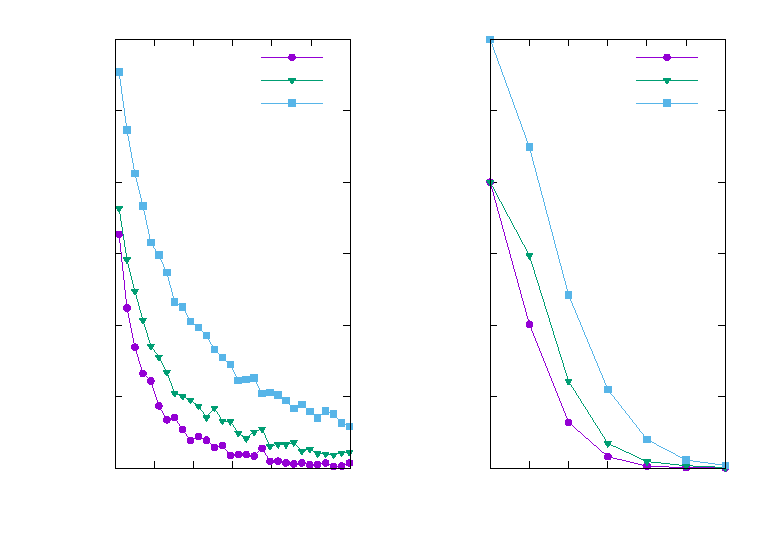
\includegraphics[width={360.00bp},height={252.00bp}]{armchair-width-strangth}}%
    \gplfronttext
  \end{picture}%
\endgroup

    \caption{(الف) رسانایی در مقابل طول روبان آرمچیر آرمچیر با عرض های مختلف (از نظر تعداد سلول های واحد در یک سوپرسل) و قدرت بی نظمی ثابت $V_d=1\;eV$. (ب) رسانایی در مقابل استحکام بی نظمی برای روبان های آرمچیر آرمچیر با بی نظمی که در هر دو لبه به طول $758.81$\AA توزیع شده است.}
    \label{armchair-width-strangth}
  \end{figure*}
  
% این فرآیند تا tn، ̃ tn ≤ δ تکرار می شود و δ به طور دلخواه کوچک است. باید توجه داشته باشیم که بعد ماتریس تعداد اتم های داخل سوپرسل است. با احتساب نمونه به عنوان بخشی از سرب سمت راست، لایه به لایه (از l=M تا l=2)، توابع سبز سطح جدید به صورت زیر یافت می شوند:
% در اینجا L (R) توابع خود انرژی هستند که اتلاف ناشی از برهمکنش با سمت چپ (راست) سازه را در نظر می گیرند.
% (الف) رسانایی نانوروبان های آرمچیر آرمچیر با عرض\AA 10.24 و طول 74.36\AA Å، با جاهای خالی واقع در لبه بالایی سوپرسل میانی نانوروبان. (ب) چگالی الکترونی حالتها در نزدیکترین محل همسایه جاهای خالی واقع شده مشابه (الف). 
% مورب اصلی ماتریس هامیلتونی هستند که با (Hl,l) نشان داده می شوند و عناصر روی دو قطر دیگر ماتریس برهمکنش مجاور دو ابرسلول به صورت (Hl,l+1) هستند. با استفاده از انرژی های خود با ابعاد مشابه با ماتریس کل هامیلتونی، تابع گرین کل نانوروبان را می توان به دست آورد. این تابع کل سبز میتواند به ویژگیهای جایگزیده در هر نقطه از نانوروبان، مانند LDOS منجر شود (شکل 9).


\subsection{اختلال ضعیف جایگزیده سازی اندرسون در نانونوارهای بورفین}
پدیده ای است که ناشی از تداخل امواج منتشر شده از مسیرهای متعدد است که در انواع سیستم های موجی قابل مشاهده است [61-65]. درک کامل جایگزیده‌سازی اندرسون امکانپذیر نخواهد بود مگر اینکه عواملی را کنترل کنیم که بر آن تأثیر میگذارند، از جمله برهمکنشهای بین ذرهای، بعد، تقارن معکوس زمانی، و ماهیت میکروسکوپی اختلال. یکی از مناسب‌ترین و قابل کنترل‌ترین نمونه‌های این امر میتواند سیستم‌های کوانتومی اتمهای فوق سرد باشد که منجر به درک عمیق جایگزیده‌سازی اندرسون میشود [66]. مکان یابی اندرسون در فیزیک حالت جامد بسیار جالب است زیرا پیش بینی می کند که یک الکترون ممکن است در یک شبکه بی نظم بی حرکت شود [67]. از قضیه بلوخ، می‌دانیم که در یک سیستم مکانیکی کوانتومی با یک همیلتونی تناوبی فضایی، حالتهای ویژه تک ذرهای در سراسر فضا گسترش یافته‌اند. وجود اختلال ایستا تقارن انتقالی کریستالی و هامیلتونی را می شکند و در نتیجه احتمال حالت‌های ویژه را افزایش می دهد که به صورت تصاعدی موضعی می شوند [68]. به طور کلی، هر چه میزان اختلال بیشتر باشد، تعداد حالتهای ویژه موضعی بیشتر میشود و در برخی موارد، زمانی که اختلال به اندازه کافی بزرگ است، همه حالت‌های گسترش یافته را به حالت‌های موضعی تبدیل میکند و باعث ترابرد اندرسون می‌شود. حالت‌های ویژه گسترده یا موضعی مربوط به حضور یا عدم وجود ذرات برای ترابرد در مقیاس طول ماکروسکوپی است. (حالتهای گسترش یافته منجر به جابجایی مربع میانگین میشود که با گذشت زمان برای مدت طولانی رشد میکند، در حالی که حالتهای موضعی رشد می‌کنند.) بنابراین، جایگزیده سازی اندرسون می‌تواند پدیده‌های ترابرد، از جمله ترابرد عایق فلزی در نیمرساناها را توضیح دهد.

در اینجا، از آنجایی که با یک سیستم شبه یک بعدی سروکار داریم، ناخالصی‌ها تنها در لبه های بالایی و پایینی نانوروبان‌ها با اختصاص یک متغیر تصادفی نامرتبط به هر یک از آنها توزیع می شوند. ناخالصی‌ها در امتداد لبه های نانوروبان توزیع می شوند و قدرت بالقوه آنها به طور تصادفی از محدوده $[-V_d, V_d]$ انتخاب می شود. همانطور که در شکل\ref{zigzagdisorder} مشاهده می شود، اگرچه پتانسیل های بسیار ضعیف رسانایی را کاهش می دهند، اما نمی توانند باعث جایگزیده سازی اندرسون شوند. همانطور که قدرت پتانسیل افزایش می یابد، واضح است که جایگزیده سازی در انرژی هایی در حدود $-0.5\;eV$ زمانی که $V_d = 2\;eV$ رخ می دهد. به عبارت دیگر، برای قدرت پتانسیل بسیار ضعیف، طول جایگزیده سازی بسیار طولانی است. این را می توان با این واقعیت توضیح داد که در یک سیستم یک بعدی بی نهایت، حتی یک اختلال بسیار ضعیف می تواند تداخل سازنده را مختل کند و باعث رسانایی صفر شود. طول جایگزیده سازی به عنوان طولی تعریف میشود که در آن همه حالتهای ویژه بلوخ به صورت فضایی گسترش یافته به حالتهای موضعی تغییر میکنند و در نتیجه رسانایی صفر میشود. همانطور که انتظار می رود، با افزایش طول نوار با قدرت پتانسیل $2 \;eV$ در لبه ها، رسانایی احتمالاً به طور تصاعدی کاهش می‌یابد. شکل\ref{zigzag-width-strangth}(a) یک رسانایی در انرژی فرمی را با میانگین بیش از 1000 پیکربندی مختلف از انتخاب های تصادفی پتانسیل در لبه‌ها برای عرض های مختلف \lr{ZBNR} نشان می دهد، که نشان دهنده کاهش نمایی در رسانایی است. در \lr{ZBNR}ها، تعداد کانالهای رسانایی در اطراف انرژی فرمی به عرض نانوروبانها بستگی دارد، که تفاوت بین رسانایی نانوروبان‌ها‌یی با طول‌های کوچک با عرض‌های مختلف را در تضاد واضح با مورد گرافن توضیح میدهد. علاوه بر این، طول طول جایگزیده سازی اندرسون در \lr{ZBNR} ها (تقریباً 180-1800 نانومتر برای عرض سلول های 4-8 واحد) بسیار بیشتر از \lr{ZGNR}ها است (تقریباً 200-800 آنگستروم که با آنچه توسط \lr{Li} و همکاران گزارش شده مطابقت دارد). [69] در گرافن). همانطور که مشاهده می شود، هر چه قدرت اختلال بیشتر باشد، طول جایگزیده سازی کوتاه‌تر به دست می آید. رسانایی \lr{ABNR} ها با عرض \lr{\AA} 10.24 و طول نانوروبان \lr{\AA} 758.81 در شکل\ref{armdisorder} نشان داده شده است. برخلاف \lr{ZBNR} ها، حتی قدرت بی نظمی بسیار ضعیف نیز ممکن است اثرات قابل توجهی بر رسانایی داشته باشد، با طول جایگزیده سازی بسیار کوتاه تر از طول جایگزیده سازی مشاهده شده در \lr{ZBNR} ها شکل\ref{armchair-width-strangth}، تغییر رسانایی در \lr{ABNR}ها را به عنوان تابعی از طول شکل\ref{armchair-width-strangth}(a) و قدرت بالقوه شکل\ref{armchair-width-strangth}(b) در انرژی انرژی فرمی، که از طریق میانگین بیش از 1000 پیکربندی مختلف اختلال لبه محاسبه شده است، نشان می دهد. هر دو شکل نشان دهنده کاهش نمایی رسانایی زمانی است که طول (یا قدرت پتانسیل) در \lr{ABNR} ها افزایش می یابد. همانطور که انتظار می رود، افزایش در تعداد کانال های رسانایی زمانی مشاهده می شود که عرض \lr{ABNR} ها افزایش می یابد، که از نظر کیفی مشابه آنچه برای \lr{ZBNR} به دست آمده است. دلیل فیزیکی پشت تاثیر بیشتر اختلال ضعیف بر هدایت \lr{ABNR} ها در مقایسه با \lr{ZBNR} ها را می توان با سرعت بالاتر سرعت گروه الکترونی در \lr{ZNBR} ها در مقایسه با \lr{ABNR} ها در محدوده انرژی فرمی درک کرد.

\begin{figure*}
\resizebox{0.95\textwidth}{!}{\includegraphics{./figures/Shematic3.png}}
\caption{به صورت شماتیک ساختار یک دریچه اسپینی مبتنی بر $\beta$-borophene را با لیدهای مغناطیسی نشان می دهد، که در آن بردارهای مغناطیسی دو لید می توانند زاویه نسبی $\theta$ داشته باشند. مغناطیسی شدن لیدها ناشی از زیرلایه مغناطیسی است که روی آن قرار می گیرند که می توان آن را به صورت تجربی کنترل کرد. در قسمت بالای شکل، بوروفن نانوروبان با لبه‌های آرمچیر و در قسمت پایین شکل، نانوروبان بوروفن زیگزاگ به تصویر کشیده شده است. سلول واحد بوروفن با اتم‌های بور که در یک بورفن لبه زیگزاگ برچسب‌گذاری شده‌اند در جدول\ref{tbl:hoppingtable} نشان داده شده است، جایی که انرژی‌های موجود در محل و پارامترهای جهش اتم‌ها آورده شده است.}
  \label{fig:model}
\end{figure*}
    
\begin{figure*}[!ht]
  \begin{latin}
  \centering
  \resizebox{0.45\textwidth}{!}{\input{./figures/Armchair-Antiparallel-conductance-revise.tex}}
  \resizebox{0.45\textwidth}{!}{% GNUPLOT: LaTeX picture with Postscript
\begin{latin}
\begingroup
  % Encoding inside the plot.  In the header of your document, this encoding
  % should to defined, e.g., by using
  % \usepackage[cp1252,<other encodings>]{inputenc}
  % \inputencoding{cp1252}%
  \makeatletter
  \providecommand\color[2][]{%
    \GenericError{(gnuplot) \space\space\space\@spaces}{%
      Package color not loaded in conjunction with
      terminal option `colourtext'%
    }{See the gnuplot documentation for explanation.%
    }{Either use 'blacktext' in gnuplot or load the package
      color.sty in LaTeX.}%
    \renewcommand\color[2][]{}%
  }%
  \providecommand\includegraphics[2][]{%
    \GenericError{(gnuplot) \space\space\space\@spaces}{%
      Package graphicx or graphics not loaded%
    }{See the gnuplot documentation for explanation.%
    }{The gnuplot epslatex terminal needs graphicx.sty or graphics.sty.}%
    \renewcommand\includegraphics[2][]{}%
  }%
  \providecommand\rotatebox[2]{#2}%
  \@ifundefined{ifGPcolor}{%
    \newif\ifGPcolor
    \GPcolorfalse
  }{}%
  \@ifundefined{ifGPblacktext}{%
    \newif\ifGPblacktext
    \GPblacktexttrue
  }{}%
  % define a \g@addto@macro without @ in the name:
  \let\gplgaddtomacro\g@addto@macro
  % define empty templates for all commands taking text:
  \gdef\gplbacktext{}%
  \gdef\gplfronttext{}%
  \makeatother
  \ifGPblacktext
    % no textcolor at all
    \def\colorrgb#1{}%
    \def\colorgray#1{}%
  \else
    % gray or color?
    \ifGPcolor
      \def\colorrgb#1{\color[rgb]{#1}}%
      \def\colorgray#1{\color[gray]{#1}}%
      \expandafter\def\csname LTw\endcsname{\color{white}}%
      \expandafter\def\csname LTb\endcsname{\color{black}}%
      \expandafter\def\csname LTa\endcsname{\color{black}}%
      \expandafter\def\csname LT0\endcsname{\color[rgb]{1,0,0}}%
      \expandafter\def\csname LT1\endcsname{\color[rgb]{0,1,0}}%
      \expandafter\def\csname LT2\endcsname{\color[rgb]{0,0,1}}%
      \expandafter\def\csname LT3\endcsname{\color[rgb]{1,0,1}}%
      \expandafter\def\csname LT4\endcsname{\color[rgb]{0,1,1}}%
      \expandafter\def\csname LT5\endcsname{\color[rgb]{1,1,0}}%
      \expandafter\def\csname LT6\endcsname{\color[rgb]{0,0,0}}%
      \expandafter\def\csname LT7\endcsname{\color[rgb]{1,0.3,0}}%
      \expandafter\def\csname LT8\endcsname{\color[rgb]{0.5,0.5,0.5}}%
    \else
      % gray
      \def\colorrgb#1{\color{black}}%
      \def\colorgray#1{\color[gray]{#1}}%
      \expandafter\def\csname LTw\endcsname{\color{white}}%
      \expandafter\def\csname LTb\endcsname{\color{black}}%
      \expandafter\def\csname LTa\endcsname{\color{black}}%
      \expandafter\def\csname LT0\endcsname{\color{black}}%
      \expandafter\def\csname LT1\endcsname{\color{black}}%
      \expandafter\def\csname LT2\endcsname{\color{black}}%
      \expandafter\def\csname LT3\endcsname{\color{black}}%
      \expandafter\def\csname LT4\endcsname{\color{black}}%
      \expandafter\def\csname LT5\endcsname{\color{black}}%
      \expandafter\def\csname LT6\endcsname{\color{black}}%
      \expandafter\def\csname LT7\endcsname{\color{black}}%
      \expandafter\def\csname LT8\endcsname{\color{black}}%
    \fi
  \fi
    \setlength{\unitlength}{0.0500bp}%
    \ifx\gptboxheight\undefined%
      \newlength{\gptboxheight}%
      \newlength{\gptboxwidth}%
      \newsavebox{\gptboxtext}%
    \fi%
    \setlength{\fboxrule}{0.5pt}%
    \setlength{\fboxsep}{1pt}%
\begin{picture}(7200.00,5040.00)%
    \gplgaddtomacro\gplbacktext{%
      \csname LTb\endcsname%%
      \put(900,4200){\makebox(0,0)[r]{\strut{}$B$}}%
      \put(550,704){\makebox(0,0)[r]{\strut{}$0$}}%
      \put(550,1112){\makebox(0,0)[r]{\strut{}$1$}}%
      \put(550,1521){\makebox(0,0)[r]{\strut{}$2$}}%
      \put(550,1929){\makebox(0,0)[r]{\strut{}$3$}}%
      \put(550,2337){\makebox(0,0)[r]{\strut{}$4$}}%
      \put(550,2746){\makebox(0,0)[r]{\strut{}$5$}}%
      \put(550,3154){\makebox(0,0)[r]{\strut{}$6$}}%
      \put(550,3562){\makebox(0,0)[r]{\strut{}$7$}}%
      \put(550,3971){\makebox(0,0)[r]{\strut{}$8$}}%
      \put(550,4379){\makebox(0,0)[r]{\strut{}$9$}}%
      \put(682,484){\makebox(0,0){\strut{}$-4$}}%
      \put(1447,484){\makebox(0,0){\strut{}$-3$}}%
      \put(2212,484){\makebox(0,0){\strut{}$-2$}}%
      \put(2977,484){\makebox(0,0){\strut{}$-1$}}%
      \put(3743,484){\makebox(0,0){\strut{}$0$}}%
      \put(4508,484){\makebox(0,0){\strut{}$1$}}%
      \put(5273,484){\makebox(0,0){\strut{}$2$}}%
      \put(6038,484){\makebox(0,0){\strut{}$3$}}%
      \put(6803,484){\makebox(0,0){\strut{}$4$}}%
    }%
    \gplgaddtomacro\gplfronttext{%
      \csname LTb\endcsname%%
      \put(209,2541){\rotatebox{-270}{\makebox(0,0){\strut{}$G(e^2/h)$}}}%
      \put(3742,154){\makebox(0,0){\strut{}$E(eV)$}}%
      \csname LTb\endcsname%%
      \put(2522,4206){\makebox(0,0)[r]{\strut{}$M=0$}}%
      \csname LTb\endcsname%%
      \put(2522,3986){\makebox(0,0)[r]{\strut{}$M=0.05$}}%
      \csname LTb\endcsname%%
      \put(4169,4206){\makebox(0,0)[r]{\strut{}$M=0.1$}}%
      \csname LTb\endcsname%%
      \put(4169,3986){\makebox(0,0)[r]{\strut{}$M=0.2$}}%
      \csname LTb\endcsname%%
      \put(5816,4206){\makebox(0,0)[r]{\strut{}$M=0.3$}}%
      \csname LTb\endcsname%%
      \put(3742,4709){\makebox(0,0){\strut{}Parallel}}%
    }%
    \gplbacktext
    \put(0,0){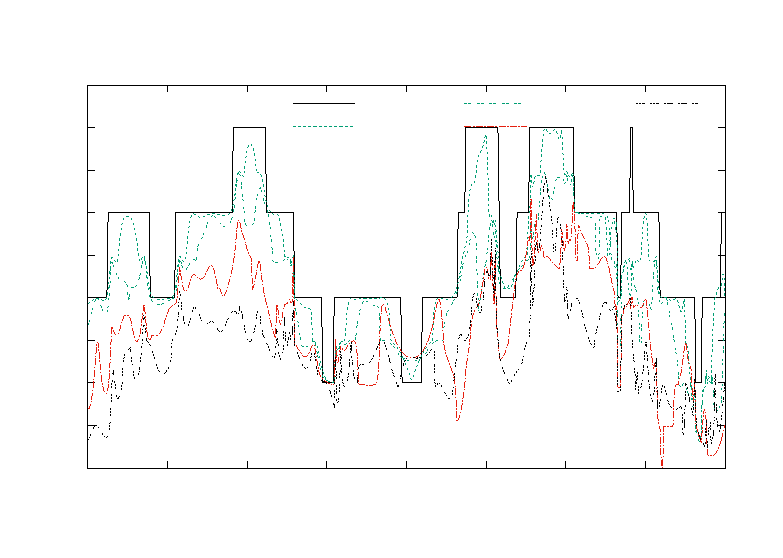
\includegraphics[width={360.00bp},height={252.00bp}]{armchair-parallel-conductance-revise}}%
    \gplfronttext
  \end{picture}%
\endgroup
\end{latin}}
  \resizebox{0.45\textwidth}{!}{% GNUPLOT: LaTeX picture with Postscript
\begingroup
  % Encoding inside the plot.  In the header of your document, this encoding
  % should to defined, e.g., by using
  % \usepackage[cp1252,<other encodings>]{inputenc}
  % \inputencoding{cp1252}%
  \makeatletter
  \providecommand\color[2][]{%
    \GenericError{(gnuplot) \space\space\space\@spaces}{%
      Package color not loaded in conjunction with
      terminal option `colourtext'%
    }{See the gnuplot documentation for explanation.%
    }{Either use 'blacktext' in gnuplot or load the package
      color.sty in LaTeX.}%
    \renewcommand\color[2][]{}%
  }%
  \providecommand\includegraphics[2][]{%
    \GenericError{(gnuplot) \space\space\space\@spaces}{%
      Package graphicx or graphics not loaded%
    }{See the gnuplot documentation for explanation.%
    }{The gnuplot epslatex terminal needs graphicx.sty or graphics.sty.}%
    \renewcommand\includegraphics[2][]{}%
  }%
  \providecommand\rotatebox[2]{#2}%
  \@ifundefined{ifGPcolor}{%
    \newif\ifGPcolor
    \GPcolorfalse
  }{}%
  \@ifundefined{ifGPblacktext}{%
    \newif\ifGPblacktext
    \GPblacktexttrue
  }{}%
  % define a \g@addto@macro without @ in the name:
  \let\gplgaddtomacro\g@addto@macro
  % define empty templates for all commands taking text:
  \gdef\gplbacktext{}%
  \gdef\gplfronttext{}%
  \makeatother
  \ifGPblacktext
    % no textcolor at all
    \def\colorrgb#1{}%
    \def\colorgray#1{}%
  \else
    % gray or color?
    \ifGPcolor
      \def\colorrgb#1{\color[rgb]{#1}}%
      \def\colorgray#1{\color[gray]{#1}}%
      \expandafter\def\csname LTw\endcsname{\color{white}}%
      \expandafter\def\csname LTb\endcsname{\color{black}}%
      \expandafter\def\csname LTa\endcsname{\color{black}}%
      \expandafter\def\csname LT0\endcsname{\color[rgb]{1,0,0}}%
      \expandafter\def\csname LT1\endcsname{\color[rgb]{0,1,0}}%
      \expandafter\def\csname LT2\endcsname{\color[rgb]{0,0,1}}%
      \expandafter\def\csname LT3\endcsname{\color[rgb]{1,0,1}}%
      \expandafter\def\csname LT4\endcsname{\color[rgb]{0,1,1}}%
      \expandafter\def\csname LT5\endcsname{\color[rgb]{1,1,0}}%
      \expandafter\def\csname LT6\endcsname{\color[rgb]{0,0,0}}%
      \expandafter\def\csname LT7\endcsname{\color[rgb]{1,0.3,0}}%
      \expandafter\def\csname LT8\endcsname{\color[rgb]{0.5,0.5,0.5}}%
    \else
      % gray
      \def\colorrgb#1{\color{black}}%
      \def\colorgray#1{\color[gray]{#1}}%
      \expandafter\def\csname LTw\endcsname{\color{white}}%
      \expandafter\def\csname LTb\endcsname{\color{black}}%
      \expandafter\def\csname LTa\endcsname{\color{black}}%
      \expandafter\def\csname LT0\endcsname{\color{black}}%
      \expandafter\def\csname LT1\endcsname{\color{black}}%
      \expandafter\def\csname LT2\endcsname{\color{black}}%
      \expandafter\def\csname LT3\endcsname{\color{black}}%
      \expandafter\def\csname LT4\endcsname{\color{black}}%
      \expandafter\def\csname LT5\endcsname{\color{black}}%
      \expandafter\def\csname LT6\endcsname{\color{black}}%
      \expandafter\def\csname LT7\endcsname{\color{black}}%
      \expandafter\def\csname LT8\endcsname{\color{black}}%
    \fi
  \fi
    \setlength{\unitlength}{0.0500bp}%
    \ifx\gptboxheight\undefined%
      \newlength{\gptboxheight}%
      \newlength{\gptboxwidth}%
      \newsavebox{\gptboxtext}%
    \fi%
    \setlength{\fboxrule}{0.5pt}%
    \setlength{\fboxsep}{1pt}%
\begin{picture}(7200.00,5040.00)%
    \gplgaddtomacro\gplbacktext{%
      \csname LTb\endcsname%%
      \put(1000,4200){\makebox(0,0)[r]{\strut{}$C$}}%
      \put(682,704){\makebox(0,0)[r]{\strut{}$2$}}%
      \put(682,1163){\makebox(0,0)[r]{\strut{}$4$}}%
      \put(682,1623){\makebox(0,0)[r]{\strut{}$6$}}%
      \put(682,2082){\makebox(0,0)[r]{\strut{}$8$}}%
      \put(682,2542){\makebox(0,0)[r]{\strut{}$10$}}%
      \put(682,3001){\makebox(0,0)[r]{\strut{}$12$}}%
      \put(682,3460){\makebox(0,0)[r]{\strut{}$14$}}%
      \put(682,3920){\makebox(0,0)[r]{\strut{}$16$}}%
      \put(682,4379){\makebox(0,0)[r]{\strut{}$18$}}%
      \put(814,484){\makebox(0,0){\strut{}$-4$}}%
      \put(1563,484){\makebox(0,0){\strut{}$-3$}}%
      \put(2311,484){\makebox(0,0){\strut{}$-2$}}%
      \put(3060,484){\makebox(0,0){\strut{}$-1$}}%
      \put(3809,484){\makebox(0,0){\strut{}$0$}}%
      \put(4557,484){\makebox(0,0){\strut{}$1$}}%
      \put(5306,484){\makebox(0,0){\strut{}$2$}}%
      \put(6054,484){\makebox(0,0){\strut{}$3$}}%
      \put(6803,484){\makebox(0,0){\strut{}$4$}}%
    }%
    \gplgaddtomacro\gplfronttext{%
      \csname LTb\endcsname%%
      \put(209,2541){\rotatebox{-270}{\makebox(0,0){\strut{}$G(e^2/h)$}}}%
      \put(3808,154){\makebox(0,0){\strut{}$E(eV)$}}%
      \csname LTb\endcsname%%
      \put(2522,4206){\makebox(0,0)[r]{\strut{}$M=0$}}%
      \csname LTb\endcsname%%
      \put(2522,3986){\makebox(0,0)[r]{\strut{}$M=0.05$}}%
      \csname LTb\endcsname%%
      \put(4169,4206){\makebox(0,0)[r]{\strut{}$M=0.1$}}%
      \csname LTb\endcsname%%
      \put(4169,3986){\makebox(0,0)[r]{\strut{}$M=0.2$}}%
      \csname LTb\endcsname%%
      \put(5816,4206){\makebox(0,0)[r]{\strut{}$M=0.3$}}%
      \csname LTb\endcsname%%
      \put(3808,4709){\makebox(0,0){\strut{}AntiParallel}}%
    }%
    \gplbacktext
    \put(0,0){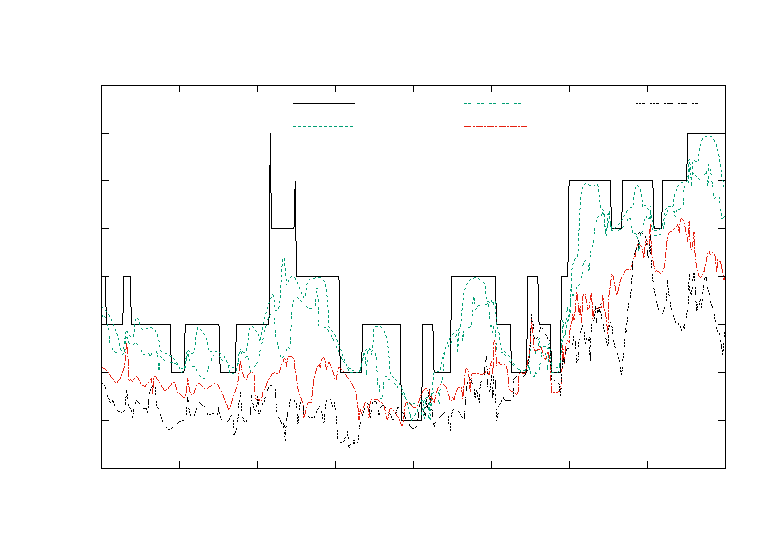
\includegraphics[width={360.00bp},height={252.00bp}]{zigzag-antiparallel-conductance-revise}}%
    \gplfronttext
  \end{picture}%
\endgroup
}
  \resizebox{0.45\textwidth}{!}{% GNUPLOT: LaTeX picture with Postscript
\begingroup
  % Encoding inside the plot.  In the header of your document, this encoding
  % should to defined, e.g., by using
  % \usepackage[cp1252,<other encodings>]{inputenc}
  % \inputencoding{cp1252}%
  \makeatletter
  \providecommand\color[2][]{%
    \GenericError{(gnuplot) \space\space\space\@spaces}{%
      Package color not loaded in conjunction with
      terminal option `colourtext'%
    }{See the gnuplot documentation for explanation.%
    }{Either use 'blacktext' in gnuplot or load the package
      color.sty in LaTeX.}%
    \renewcommand\color[2][]{}%
  }%
  \providecommand\includegraphics[2][]{%
    \GenericError{(gnuplot) \space\space\space\@spaces}{%
      Package graphicx or graphics not loaded%
    }{See the gnuplot documentation for explanation.%
    }{The gnuplot epslatex terminal needs graphicx.sty or graphics.sty.}%
    \renewcommand\includegraphics[2][]{}%
  }%
  \providecommand\rotatebox[2]{#2}%
  \@ifundefined{ifGPcolor}{%
    \newif\ifGPcolor
    \GPcolorfalse
  }{}%
  \@ifundefined{ifGPblacktext}{%
    \newif\ifGPblacktext
    \GPblacktexttrue
  }{}%
  % define a \g@addto@macro without @ in the name:
  \let\gplgaddtomacro\g@addto@macro
  % define empty templates for all commands taking text:
  \gdef\gplbacktext{}%
  \gdef\gplfronttext{}%
  \makeatother
  \ifGPblacktext
    % no textcolor at all
    \def\colorrgb#1{}%
    \def\colorgray#1{}%
  \else
    % gray or color?
    \ifGPcolor
      \def\colorrgb#1{\color[rgb]{#1}}%
      \def\colorgray#1{\color[gray]{#1}}%
      \expandafter\def\csname LTw\endcsname{\color{white}}%
      \expandafter\def\csname LTb\endcsname{\color{black}}%
      \expandafter\def\csname LTa\endcsname{\color{black}}%
      \expandafter\def\csname LT0\endcsname{\color[rgb]{1,0,0}}%
      \expandafter\def\csname LT1\endcsname{\color[rgb]{0,1,0}}%
      \expandafter\def\csname LT2\endcsname{\color[rgb]{0,0,1}}%
      \expandafter\def\csname LT3\endcsname{\color[rgb]{1,0,1}}%
      \expandafter\def\csname LT4\endcsname{\color[rgb]{0,1,1}}%
      \expandafter\def\csname LT5\endcsname{\color[rgb]{1,1,0}}%
      \expandafter\def\csname LT6\endcsname{\color[rgb]{0,0,0}}%
      \expandafter\def\csname LT7\endcsname{\color[rgb]{1,0.3,0}}%
      \expandafter\def\csname LT8\endcsname{\color[rgb]{0.5,0.5,0.5}}%
    \else
      % gray
      \def\colorrgb#1{\color{black}}%
      \def\colorgray#1{\color[gray]{#1}}%
      \expandafter\def\csname LTw\endcsname{\color{white}}%
      \expandafter\def\csname LTb\endcsname{\color{black}}%
      \expandafter\def\csname LTa\endcsname{\color{black}}%
      \expandafter\def\csname LT0\endcsname{\color{black}}%
      \expandafter\def\csname LT1\endcsname{\color{black}}%
      \expandafter\def\csname LT2\endcsname{\color{black}}%
      \expandafter\def\csname LT3\endcsname{\color{black}}%
      \expandafter\def\csname LT4\endcsname{\color{black}}%
      \expandafter\def\csname LT5\endcsname{\color{black}}%
      \expandafter\def\csname LT6\endcsname{\color{black}}%
      \expandafter\def\csname LT7\endcsname{\color{black}}%
      \expandafter\def\csname LT8\endcsname{\color{black}}%
    \fi
  \fi
    \setlength{\unitlength}{0.0500bp}%
    \ifx\gptboxheight\undefined%
      \newlength{\gptboxheight}%
      \newlength{\gptboxwidth}%
      \newsavebox{\gptboxtext}%
    \fi%
    \setlength{\fboxrule}{0.5pt}%
    \setlength{\fboxsep}{1pt}%
\begin{picture}(7200.00,5040.00)%
    \gplgaddtomacro\gplbacktext{%
      \csname LTb\endcsname%%
      \put(1000,4200){\makebox(0,0)[r]{\strut{}$D$}}%
      \put(682,704){\makebox(0,0)[r]{\strut{}$0$}}%
      \put(682,1112){\makebox(0,0)[r]{\strut{}$2$}}%
      \put(682,1521){\makebox(0,0)[r]{\strut{}$4$}}%
      \put(682,1929){\makebox(0,0)[r]{\strut{}$6$}}%
      \put(682,2337){\makebox(0,0)[r]{\strut{}$8$}}%
      \put(682,2746){\makebox(0,0)[r]{\strut{}$10$}}%
      \put(682,3154){\makebox(0,0)[r]{\strut{}$12$}}%
      \put(682,3562){\makebox(0,0)[r]{\strut{}$14$}}%
      \put(682,3971){\makebox(0,0)[r]{\strut{}$16$}}%
      \put(682,4379){\makebox(0,0)[r]{\strut{}$18$}}%
      \put(814,484){\makebox(0,0){\strut{}$-4$}}%
      \put(1563,484){\makebox(0,0){\strut{}$-3$}}%
      \put(2311,484){\makebox(0,0){\strut{}$-2$}}%
      \put(3060,484){\makebox(0,0){\strut{}$-1$}}%
      \put(3809,484){\makebox(0,0){\strut{}$0$}}%
      \put(4557,484){\makebox(0,0){\strut{}$1$}}%
      \put(5306,484){\makebox(0,0){\strut{}$2$}}%
      \put(6054,484){\makebox(0,0){\strut{}$3$}}%
      \put(6803,484){\makebox(0,0){\strut{}$4$}}%
    }%
    \gplgaddtomacro\gplfronttext{%
      \csname LTb\endcsname%%
      \put(209,2541){\rotatebox{-270}{\makebox(0,0){\strut{}$G(e^2/h)$}}}%
      \put(3808,154){\makebox(0,0){\strut{}$E(eV)$}}%
      \csname LTb\endcsname%%
      \put(2522,4206){\makebox(0,0)[r]{\strut{}$M=0$}}%
      \csname LTb\endcsname%%
      \put(2522,3986){\makebox(0,0)[r]{\strut{}$M=0.05$}}%
      \csname LTb\endcsname%%
      \put(4169,4206){\makebox(0,0)[r]{\strut{}$M=0.1$}}%
      \csname LTb\endcsname%%
      \put(4169,3986){\makebox(0,0)[r]{\strut{}$M=0.2$}}%
      \csname LTb\endcsname%%
      \put(5816,4206){\makebox(0,0)[r]{\strut{}$M=0.3$}}%
      \csname LTb\endcsname%%
      \put(3808,4709){\makebox(0,0){\strut{}Parallel}}%
    }%
    \gplbacktext
    \put(0,0){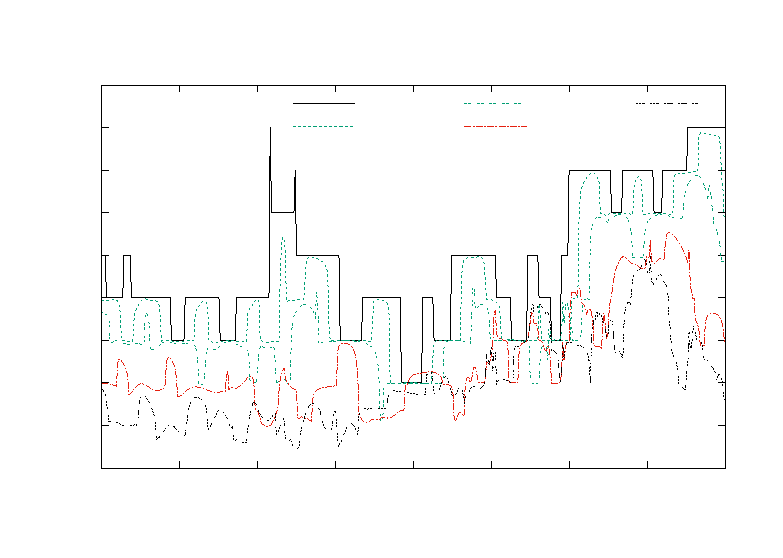
\includegraphics[width={360.00bp},height={252.00bp}]{zigzag-parallel-conductance-revise}}%
    \gplfronttext
  \end{picture}%
\endgroup
}  
  \end{latin}
\caption{الف) پلات بوروفن با لبه آرمچیر با عرض 4 سلول برای مغناطش متفاوت لیدها در پیکربندی AP. ب) رسم بوروفن با لبه آرمچیر، و عرض سلول 4 واحد، برای مغناطش متفاوت لیدها در پیکربندی P. ج) نمودار بوروفن با لبه زیگزاگ، با عرض سلول 4 واحد، برای مغناطش متفاوت لیدها در پیکربندی P. د) رسم بوروفن با لبه زیگزاگ و عرض سلول 4 واحد، برای مغناطش متفاوت لیدها در پیکربندی AP.}
\label{fig:conductance}
\end{figure*}
\begin{figure*}[!ht]
  \begin{latin}
    \centering
    \resizebox{0.32\textwidth}{!}{% GNUPLOT: LaTeX picture with Postscript
\begin{latin}
\begingroup
  \makeatletter
  \providecommand\color[2][]{%
    \GenericError{(gnuplot) \space\space\space\@spaces}{%
      Package color not loaded in conjunction with
      terminal option `colourtext'%
    }{See the gnuplot documentation for explanation.%
    }{Either use 'blacktext' in gnuplot or load the package
      color.sty in LaTeX.}%
    \renewcommand\color[2][]{}%
  }%
  \providecommand\includegraphics[2][]{%
    \GenericError{(gnuplot) \space\space\space\@spaces}{%
      Package graphicx or graphics not loaded%
    }{See the gnuplot documentation for explanation.%
    }{The gnuplot epslatex terminal needs graphicx.sty or graphics.sty.}%
    \renewcommand\includegraphics[2][]{}%
  }%
  \providecommand\rotatebox[2]{#2}%
  \@ifundefined{ifGPcolor}{%
    \newif\ifGPcolor
    \GPcolorfalse
  }{}%
  \@ifundefined{ifGPblacktext}{%
    \newif\ifGPblacktext
    \GPblacktexttrue
  }{}%
  % define a \g@addto@macro without @ in the name:
  \let\gplgaddtomacro\g@addto@macro
  % define empty templates for all commands taking text:
  \gdef\gplbacktext{}%
  \gdef\gplfronttext{}%
  \makeatother
  \ifGPblacktext
    % no textcolor at all
    \def\colorrgb#1{}%
    \def\colorgray#1{}%
  \else
    % gray or color?
    \ifGPcolor
      \def\colorrgb#1{\color[rgb]{#1}}%
      \def\colorgray#1{\color[gray]{#1}}%
      \expandafter\def\csname LTw\endcsname{\color{white}}%
      \expandafter\def\csname LTb\endcsname{\color{black}}%
      \expandafter\def\csname LTa\endcsname{\color{black}}%
      \expandafter\def\csname LT0\endcsname{\color[rgb]{1,0,0}}%
      \expandafter\def\csname LT1\endcsname{\color[rgb]{0,1,0}}%
      \expandafter\def\csname LT2\endcsname{\color[rgb]{0,0,1}}%
      \expandafter\def\csname LT3\endcsname{\color[rgb]{1,0,1}}%
      \expandafter\def\csname LT4\endcsname{\color[rgb]{0,1,1}}%
      \expandafter\def\csname LT5\endcsname{\color[rgb]{1,1,0}}%
      \expandafter\def\csname LT6\endcsname{\color[rgb]{0,0,0}}%
      \expandafter\def\csname LT7\endcsname{\color[rgb]{1,0.3,0}}%
      \expandafter\def\csname LT8\endcsname{\color[rgb]{0.5,0.5,0.5}}%
    \else
      % gray
      \def\colorrgb#1{\color{black}}%
      \def\colorgray#1{\color[gray]{#1}}%
      \expandafter\def\csname LTw\endcsname{\color{white}}%
      \expandafter\def\csname LTb\endcsname{\color{black}}%
      \expandafter\def\csname LTa\endcsname{\color{black}}%
      \expandafter\def\csname LT0\endcsname{\color{black}}%
      \expandafter\def\csname LT1\endcsname{\color{black}}%
      \expandafter\def\csname LT2\endcsname{\color{black}}%
      \expandafter\def\csname LT3\endcsname{\color{black}}%
      \expandafter\def\csname LT4\endcsname{\color{black}}%
      \expandafter\def\csname LT5\endcsname{\color{black}}%
      \expandafter\def\csname LT6\endcsname{\color{black}}%
      \expandafter\def\csname LT7\endcsname{\color{black}}%
      \expandafter\def\csname LT8\endcsname{\color{black}}%
    \fi
  \fi
    \setlength{\unitlength}{0.0500bp}%
    \ifx\gptboxheight\undefined%
      \newlength{\gptboxheight}%
      \newlength{\gptboxwidth}%
      \newsavebox{\gptboxtext}%
    \fi%
    \setlength{\fboxrule}{0.5pt}%
    \setlength{\fboxsep}{1pt}%
\begin{picture}(3600.00,5040.00)%
    \gplgaddtomacro\gplbacktext{%
      \csname LTb\endcsname%%
      \put(1450,4200){\makebox(0,0)[r]{\strut{}$A$}}%
      \put(946,704){\makebox(0,0)[r]{\strut{}$-0.8$}}%
      \put(946,1439){\makebox(0,0)[r]{\strut{}$-0.7$}}%
      \put(946,2174){\makebox(0,0)[r]{\strut{}$-0.6$}}%
      \put(946,2909){\makebox(0,0)[r]{\strut{}$-0.5$}}%
      \put(946,3644){\makebox(0,0)[r]{\strut{}$-0.4$}}%
      \put(946,4379){\makebox(0,0)[r]{\strut{}$-0.3$}}%
      \put(1078,484){\makebox(0,0){\strut{}$0$}}%
      \put(1609,484){\makebox(0,0){\strut{}$0.5$}}%
      \put(2141,484){\makebox(0,0){\strut{}$1$}}%
      \put(2672,484){\makebox(0,0){\strut{}$1.5$}}%
      \put(3203,484){\makebox(0,0){\strut{}$2$}}%
      \put(1089,2909){\makebox(0,0)[l]{\strut{}$8\uparrow$}}%
      \put(1344,1439){\makebox(0,0)[l]{\strut{}$8\downarrow$}}%
      \put(1482,2909){\makebox(0,0)[l]{\strut{}$9\uparrow$}}%
      \put(1981,2174){\makebox(0,0)[l]{\strut{}$9\downarrow$}}%
    }%
    \gplgaddtomacro\gplfronttext{%
      \csname LTb\endcsname%%
      \put(209,2541){\rotatebox{-270}{\makebox(0,0){\strut{}$E(eV)$}}}%
      \put(2140,154){\makebox(0,0){\strut{}$k_x$}}%
      \csname LTb\endcsname%%
      \put(2140,4709){\makebox(0,0){\strut{}Left}}%
    }%
    \gplbacktext
    \put(0,0){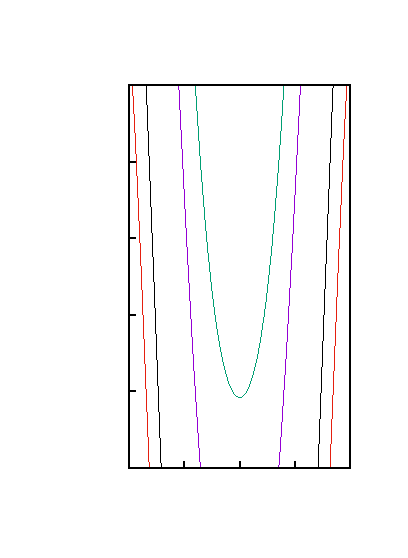
\includegraphics[width={180.00bp},height={252.00bp}]{Lborophene_band-revised}}%
    \gplfronttext
  \end{picture}%
\endgroup
\end{latin}}
    \resizebox{0.32\textwidth}{!}{% GNUPLOT: LaTeX picture with Postscript
\begin{latin}
\begingroup
  \makeatletter
  \providecommand\color[2][]{%
    \GenericError{(gnuplot) \space\space\space\@spaces}{%
      Package color not loaded in conjunction with
      terminal option `colourtext'%
    }{See the gnuplot documentation for explanation.%
    }{Either use 'blacktext' in gnuplot or load the package
      color.sty in LaTeX.}%
    \renewcommand\color[2][]{}%
  }%
  \providecommand\includegraphics[2][]{%
    \GenericError{(gnuplot) \space\space\space\@spaces}{%
      Package graphicx or graphics not loaded%
    }{See the gnuplot documentation for explanation.%
    }{The gnuplot epslatex terminal needs graphicx.sty or graphics.sty.}%
    \renewcommand\includegraphics[2][]{}%
  }%
  \providecommand\rotatebox[2]{#2}%
  \@ifundefined{ifGPcolor}{%
    \newif\ifGPcolor
    \GPcolorfalse
  }{}%
  \@ifundefined{ifGPblacktext}{%
    \newif\ifGPblacktext
    \GPblacktexttrue
  }{}%
  % define a \g@addto@macro without @ in the name:
  \let\gplgaddtomacro\g@addto@macro
  % define empty templates for all commands taking text:
  \gdef\gplbacktext{}%
  \gdef\gplfronttext{}%
  \makeatother
  \ifGPblacktext
    % no textcolor at all
    \def\colorrgb#1{}%
    \def\colorgray#1{}%
  \else
    % gray or color?
    \ifGPcolor
      \def\colorrgb#1{\color[rgb]{#1}}%
      \def\colorgray#1{\color[gray]{#1}}%
      \expandafter\def\csname LTw\endcsname{\color{white}}%
      \expandafter\def\csname LTb\endcsname{\color{black}}%
      \expandafter\def\csname LTa\endcsname{\color{black}}%
      \expandafter\def\csname LT0\endcsname{\color[rgb]{1,0,0}}%
      \expandafter\def\csname LT1\endcsname{\color[rgb]{0,1,0}}%
      \expandafter\def\csname LT2\endcsname{\color[rgb]{0,0,1}}%
      \expandafter\def\csname LT3\endcsname{\color[rgb]{1,0,1}}%
      \expandafter\def\csname LT4\endcsname{\color[rgb]{0,1,1}}%
      \expandafter\def\csname LT5\endcsname{\color[rgb]{1,1,0}}%
      \expandafter\def\csname LT6\endcsname{\color[rgb]{0,0,0}}%
      \expandafter\def\csname LT7\endcsname{\color[rgb]{1,0.3,0}}%
      \expandafter\def\csname LT8\endcsname{\color[rgb]{0.5,0.5,0.5}}%
    \else
      % gray
      \def\colorrgb#1{\color{black}}%
      \def\colorgray#1{\color[gray]{#1}}%
      \expandafter\def\csname LTw\endcsname{\color{white}}%
      \expandafter\def\csname LTb\endcsname{\color{black}}%
      \expandafter\def\csname LTa\endcsname{\color{black}}%
      \expandafter\def\csname LT0\endcsname{\color{black}}%
      \expandafter\def\csname LT1\endcsname{\color{black}}%
      \expandafter\def\csname LT2\endcsname{\color{black}}%
      \expandafter\def\csname LT3\endcsname{\color{black}}%
      \expandafter\def\csname LT4\endcsname{\color{black}}%
      \expandafter\def\csname LT5\endcsname{\color{black}}%
      \expandafter\def\csname LT6\endcsname{\color{black}}%
      \expandafter\def\csname LT7\endcsname{\color{black}}%
      \expandafter\def\csname LT8\endcsname{\color{black}}%
    \fi
  \fi
    \setlength{\unitlength}{0.0500bp}%
    \ifx\gptboxheight\undefined%
      \newlength{\gptboxheight}%
      \newlength{\gptboxwidth}%
      \newsavebox{\gptboxtext}%
    \fi%
    \setlength{\fboxrule}{0.5pt}%
    \setlength{\fboxsep}{1pt}%
\begin{picture}(3600.00,5040.00)%
    \gplgaddtomacro\gplbacktext{%
      \csname LTb\endcsname%%
      \put(1400,4200){\makebox(0,0)[r]{\strut{}$B$}}%
      \put(946,704){\makebox(0,0)[r]{\strut{}$-0.8$}}%
      \put(946,1439){\makebox(0,0)[r]{\strut{}$-0.7$}}%
      \put(946,2174){\makebox(0,0)[r]{\strut{}$-0.6$}}%
      \put(946,2909){\makebox(0,0)[r]{\strut{}$-0.5$}}%
      \put(946,3644){\makebox(0,0)[r]{\strut{}$-0.4$}}%
      \put(946,4379){\makebox(0,0)[r]{\strut{}$-0.3$}}%
      \put(1078,484){\makebox(0,0){\strut{}$0$}}%
      \put(1609,484){\makebox(0,0){\strut{}$0.5$}}%
      \put(2141,484){\makebox(0,0){\strut{}$1$}}%
      \put(2672,484){\makebox(0,0){\strut{}$1.5$}}%
      \put(3203,484){\makebox(0,0){\strut{}$2$}}%
      \put(1089,2909){\makebox(0,0)[l]{\strut{}$8\uparrow$}}%
      \put(1344,1439){\makebox(0,0)[l]{\strut{}$8\downarrow$}}%
      \put(1482,2909){\makebox(0,0)[l]{\strut{}$9\uparrow$}}%
      \put(1981,2174){\makebox(0,0)[l]{\strut{}$9\downarrow$}}%
    }%
    \gplgaddtomacro\gplfronttext{%
      \csname LTb\endcsname%%
      \put(209,2541){\rotatebox{-270}{\makebox(0,0){\strut{}$E(eV)$}}}%
      \put(2140,154){\makebox(0,0){\strut{}$k_x$}}%
      \csname LTb\endcsname%%
      \put(2140,4709){\makebox(0,0){\strut{}Center}}%
    }%
    \gplbacktext
    \put(0,0){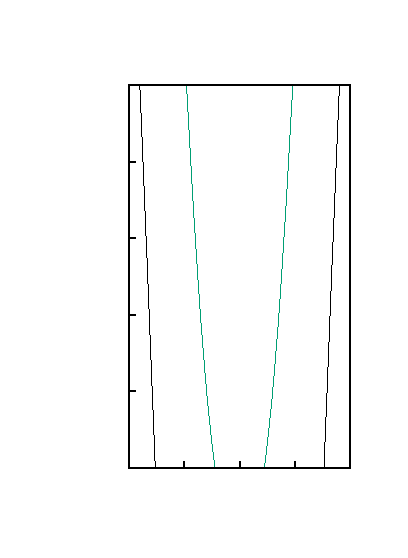
\includegraphics[width={180.00bp},height={252.00bp}]{Cborophene_band-revised}}%
    \gplfronttext
  \end{picture}%
\endgroup
\end{latin}}
    \resizebox{0.32\textwidth}{!}{% GNUPLOT: LaTeX picture with Postscript
\begingroup
  \makeatletter
  \providecommand\color[2][]{%
    \GenericError{(gnuplot) \space\space\space\@spaces}{%
      Package color not loaded in conjunction with
      terminal option `colourtext'%
    }{See the gnuplot documentation for explanation.%
    }{Either use 'blacktext' in gnuplot or load the package
      color.sty in LaTeX.}%
    \renewcommand\color[2][]{}%
  }%
  \providecommand\includegraphics[2][]{%
    \GenericError{(gnuplot) \space\space\space\@spaces}{%
      Package graphicx or graphics not loaded%
    }{See the gnuplot documentation for explanation.%
    }{The gnuplot epslatex terminal needs graphicx.sty or graphics.sty.}%
    \renewcommand\includegraphics[2][]{}%
  }%
  \providecommand\rotatebox[2]{#2}%
  \@ifundefined{ifGPcolor}{%
    \newif\ifGPcolor
    \GPcolorfalse
  }{}%
  \@ifundefined{ifGPblacktext}{%
    \newif\ifGPblacktext
    \GPblacktexttrue
  }{}%
  % define a \g@addto@macro without @ in the name:
  \let\gplgaddtomacro\g@addto@macro
  % define empty templates for all commands taking text:
  \gdef\gplbacktext{}%
  \gdef\gplfronttext{}%
  \makeatother
  \ifGPblacktext
    % no textcolor at all
    \def\colorrgb#1{}%
    \def\colorgray#1{}%
  \else
    % gray or color?
    \ifGPcolor
      \def\colorrgb#1{\color[rgb]{#1}}%
      \def\colorgray#1{\color[gray]{#1}}%
      \expandafter\def\csname LTw\endcsname{\color{white}}%
      \expandafter\def\csname LTb\endcsname{\color{black}}%
      \expandafter\def\csname LTa\endcsname{\color{black}}%
      \expandafter\def\csname LT0\endcsname{\color[rgb]{1,0,0}}%
      \expandafter\def\csname LT1\endcsname{\color[rgb]{0,1,0}}%
      \expandafter\def\csname LT2\endcsname{\color[rgb]{0,0,1}}%
      \expandafter\def\csname LT3\endcsname{\color[rgb]{1,0,1}}%
      \expandafter\def\csname LT4\endcsname{\color[rgb]{0,1,1}}%
      \expandafter\def\csname LT5\endcsname{\color[rgb]{1,1,0}}%
      \expandafter\def\csname LT6\endcsname{\color[rgb]{0,0,0}}%
      \expandafter\def\csname LT7\endcsname{\color[rgb]{1,0.3,0}}%
      \expandafter\def\csname LT8\endcsname{\color[rgb]{0.5,0.5,0.5}}%
    \else
      % gray
      \def\colorrgb#1{\color{black}}%
      \def\colorgray#1{\color[gray]{#1}}%
      \expandafter\def\csname LTw\endcsname{\color{white}}%
      \expandafter\def\csname LTb\endcsname{\color{black}}%
      \expandafter\def\csname LTa\endcsname{\color{black}}%
      \expandafter\def\csname LT0\endcsname{\color{black}}%
      \expandafter\def\csname LT1\endcsname{\color{black}}%
      \expandafter\def\csname LT2\endcsname{\color{black}}%
      \expandafter\def\csname LT3\endcsname{\color{black}}%
      \expandafter\def\csname LT4\endcsname{\color{black}}%
      \expandafter\def\csname LT5\endcsname{\color{black}}%
      \expandafter\def\csname LT6\endcsname{\color{black}}%
      \expandafter\def\csname LT7\endcsname{\color{black}}%
      \expandafter\def\csname LT8\endcsname{\color{black}}%
    \fi
  \fi
    \setlength{\unitlength}{0.0500bp}%
    \ifx\gptboxheight\undefined%
      \newlength{\gptboxheight}%
      \newlength{\gptboxwidth}%
      \newsavebox{\gptboxtext}%
    \fi%
    \setlength{\fboxrule}{0.5pt}%
    \setlength{\fboxsep}{1pt}%
\begin{picture}(3600.00,5040.00)%
    \gplgaddtomacro\gplbacktext{%
      \csname LTb\endcsname%%
      \put(1450,4200){\makebox(0,0)[r]{\strut{}$C$}}%
      \put(946,704){\makebox(0,0)[r]{\strut{}$-0.8$}}%
      \put(946,1439){\makebox(0,0)[r]{\strut{}$-0.7$}}%
      \put(946,2174){\makebox(0,0)[r]{\strut{}$-0.6$}}%
      \put(946,2909){\makebox(0,0)[r]{\strut{}$-0.5$}}%
      \put(946,3644){\makebox(0,0)[r]{\strut{}$-0.4$}}%
      \put(946,4379){\makebox(0,0)[r]{\strut{}$-0.3$}}%
      \put(1078,484){\makebox(0,0){\strut{}$0$}}%
      \put(1609,484){\makebox(0,0){\strut{}$0.5$}}%
      \put(2141,484){\makebox(0,0){\strut{}$1$}}%
      \put(2672,484){\makebox(0,0){\strut{}$1.5$}}%
      \put(3203,484){\makebox(0,0){\strut{}$2$}}%
      \put(1089,2909){\makebox(0,0)[l]{\strut{}$8\uparrow$}}%
      \put(1344,1439){\makebox(0,0)[l]{\strut{}$8\downarrow$}}%
      \put(1482,2909){\makebox(0,0)[l]{\strut{}$9\uparrow$}}%
      \put(1981,2174){\makebox(0,0)[l]{\strut{}$9\downarrow$}}%
    }%
    \gplgaddtomacro\gplfronttext{%
      \csname LTb\endcsname%%
      \put(209,2541){\rotatebox{-270}{\makebox(0,0){\strut{}$E(eV)$}}}%
      \put(2140,154){\makebox(0,0){\strut{}$k_x$}}%
      \csname LTb\endcsname%%
      \put(2140,4709){\makebox(0,0){\strut{}Right}}%
    }%
    \gplbacktext
    \put(0,0){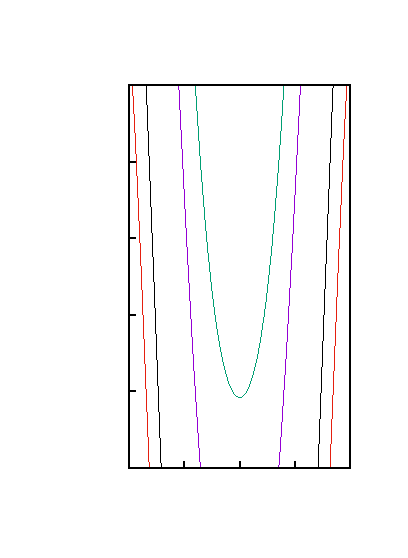
\includegraphics[width={180.00bp},height={252.00bp}]{Rborophene_band-revised}}%
    \gplfronttext
  \end{picture}%
\endgroup
}
    \resizebox{0.45\textwidth}{!}{% GNUPLOT: LaTeX picture with Postscript
\begin{latin}
\begingroup
  % Encoding inside the plot.  In the header of your document, this encoding
  % should to defined, e.g., by using
  % \usepackage[cp1252,<other encodings>]{inputenc}
  % \inputencoding{cp1252}%
  \makeatletter
  \providecommand\color[2][]{%
    \GenericError{(gnuplot) \space\space\space\@spaces}{%
      Package color not loaded in conjunction with
      terminal option `colourtext'%
    }{See the gnuplot documentation for explanation.%
    }{Either use 'blacktext' in gnuplot or load the package
      color.sty in LaTeX.}%
    \renewcommand\color[2][]{}%
  }%
  \providecommand\includegraphics[2][]{%
    \GenericError{(gnuplot) \space\space\space\@spaces}{%
      Package graphicx or graphics not loaded%
    }{See the gnuplot documentation for explanation.%
    }{The gnuplot epslatex terminal needs graphicx.sty or graphics.sty.}%
    \renewcommand\includegraphics[2][]{}%
  }%
  \providecommand\rotatebox[2]{#2}%
  \@ifundefined{ifGPcolor}{%
    \newif\ifGPcolor
    \GPcolorfalse
  }{}%
  \@ifundefined{ifGPblacktext}{%
    \newif\ifGPblacktext
    \GPblacktexttrue
  }{}%
  % define a \g@addto@macro without @ in the name:
  \let\gplgaddtomacro\g@addto@macro
  % define empty templates for all commands taking text:
  \gdef\gplbacktext{}%
  \gdef\gplfronttext{}%
  \makeatother
  \ifGPblacktext
    % no textcolor at all
    \def\colorrgb#1{}%
    \def\colorgray#1{}%
  \else
    % gray or color?
    \ifGPcolor
      \def\colorrgb#1{\color[rgb]{#1}}%
      \def\colorgray#1{\color[gray]{#1}}%
      \expandafter\def\csname LTw\endcsname{\color{white}}%
      \expandafter\def\csname LTb\endcsname{\color{black}}%
      \expandafter\def\csname LTa\endcsname{\color{black}}%
      \expandafter\def\csname LT0\endcsname{\color[rgb]{1,0,0}}%
      \expandafter\def\csname LT1\endcsname{\color[rgb]{0,1,0}}%
      \expandafter\def\csname LT2\endcsname{\color[rgb]{0,0,1}}%
      \expandafter\def\csname LT3\endcsname{\color[rgb]{1,0,1}}%
      \expandafter\def\csname LT4\endcsname{\color[rgb]{0,1,1}}%
      \expandafter\def\csname LT5\endcsname{\color[rgb]{1,1,0}}%
      \expandafter\def\csname LT6\endcsname{\color[rgb]{0,0,0}}%
      \expandafter\def\csname LT7\endcsname{\color[rgb]{1,0.3,0}}%
      \expandafter\def\csname LT8\endcsname{\color[rgb]{0.5,0.5,0.5}}%
    \else
      % gray
      \def\colorrgb#1{\color{black}}%
      \def\colorgray#1{\color[gray]{#1}}%
      \expandafter\def\csname LTw\endcsname{\color{white}}%
      \expandafter\def\csname LTb\endcsname{\color{black}}%
      \expandafter\def\csname LTa\endcsname{\color{black}}%
      \expandafter\def\csname LT0\endcsname{\color{black}}%
      \expandafter\def\csname LT1\endcsname{\color{black}}%
      \expandafter\def\csname LT2\endcsname{\color{black}}%
      \expandafter\def\csname LT3\endcsname{\color{black}}%
      \expandafter\def\csname LT4\endcsname{\color{black}}%
      \expandafter\def\csname LT5\endcsname{\color{black}}%
      \expandafter\def\csname LT6\endcsname{\color{black}}%
      \expandafter\def\csname LT7\endcsname{\color{black}}%
      \expandafter\def\csname LT8\endcsname{\color{black}}%
    \fi
  \fi
    \setlength{\unitlength}{0.0500bp}%
    \ifx\gptboxheight\undefined%
      \newlength{\gptboxheight}%
      \newlength{\gptboxwidth}%
      \newsavebox{\gptboxtext}%
    \fi%
    \setlength{\fboxrule}{0.5pt}%
    \setlength{\fboxsep}{1pt}%
\begin{picture}(7200.00,5040.00)%
    \gplgaddtomacro\gplbacktext{%
      \csname LTb\endcsname%%
      \put(1200,4200){\makebox(0,0)[r]{\strut{}$D$}}%
      \put(814,704){\makebox(0,0)[r]{\strut{}$1$}}%
      \put(814,1229){\makebox(0,0)[r]{\strut{}$1.5$}}%
      \put(814,1754){\makebox(0,0)[r]{\strut{}$2$}}%
      \put(814,2279){\makebox(0,0)[r]{\strut{}$2.5$}}%
      \put(814,2804){\makebox(0,0)[r]{\strut{}$3$}}%
      \put(814,3329){\makebox(0,0)[r]{\strut{}$3.5$}}%
      \put(814,3854){\makebox(0,0)[r]{\strut{}$4$}}%
      \put(814,4379){\makebox(0,0)[r]{\strut{}$4.5$}}%
      \put(946,484){\makebox(0,0){\strut{}$-1$}}%
      \put(2117,484){\makebox(0,0){\strut{}$-0.8$}}%
      \put(3289,484){\makebox(0,0){\strut{}$-0.6$}}%
      \put(4460,484){\makebox(0,0){\strut{}$-0.4$}}%
      \put(5632,484){\makebox(0,0){\strut{}$-0.2$}}%
      \put(6803,484){\makebox(0,0){\strut{}$0$}}%
    }%
    \gplgaddtomacro\gplfronttext{%
      \csname LTb\endcsname%%
      \put(209,2541){\rotatebox{-270}{\makebox(0,0){\strut{}$G(e^2/h)$}}}%
      \put(3874,154){\makebox(0,0){\strut{}$E(eV)$}}%
      \csname LTb\endcsname%%
      \put(2522,4206){\makebox(0,0)[r]{\strut{}$M=0$}}%
      \csname LTb\endcsname%%
      \put(2522,3986){\makebox(0,0)[r]{\strut{}$M=0.05$}}%
      \csname LTb\endcsname%%
      \put(4169,4206){\makebox(0,0)[r]{\strut{}$M=0.1$}}%
      \csname LTb\endcsname%%
      \put(4169,3986){\makebox(0,0)[r]{\strut{}$M=0.2$}}%
      \csname LTb\endcsname%%
      \put(5816,4206){\makebox(0,0)[r]{\strut{}$M=0.3$}}%
      \csname LTb\endcsname%%
      \put(3874,4709){\makebox(0,0){\strut{}Parallel}}%
    }%
    \gplbacktext
    \put(0,0){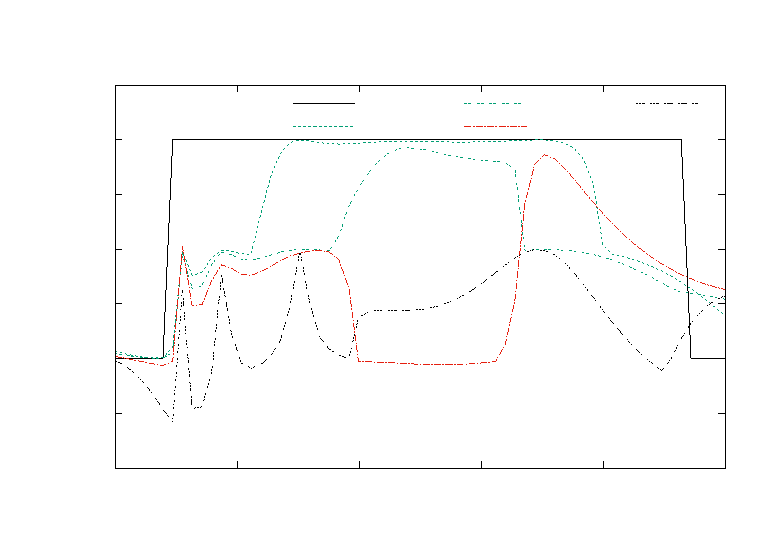
\includegraphics[width={360.00bp},height={252.00bp}]{armchair-parallel-conductance-1to0-revise}}%
    \gplfronttext
  \end{picture}%
\endgroup
\end{latin}}
    \resizebox{0.45\textwidth}{!}{\input{./figures/armchair-Antiparallel-conductance-1to0-revise.tex}}
  \end{latin}
\caption{A, B, C) در لید سمت چپ، برای تعداد زوج اتم در سوپرسل، برای مثال، نوار شماره 8 (یا 9) با عدد اتم $8(9)$ مطابقت دارد که به دو زیر‌نوار spin up $ تقسیم می شود. (8^\uparrow)$ و وقتی تعامل اسپین گنجانده شده است، $(8\downarrow)$ را به پایین بچرخانید: الف) در پیکربندی P، زیر‌نوارهای $(8\uparrow)$ در هر دو لید چپ و راست در بالای زیر‌نوارهای $(8\downarrow)$ با پاریته یکسان است و بنابراین ترابرد الکترون مجاز است. ب) در پیکربندی‌های AP، $(8\uparrow)$، در یک لید، بالاتر از زیر‌نوار $(8\downarrow)$ در همان لید قرار دارد، در حالی که در لید دیگر، $(8\uparrow) $ در زیر‌نوار $(8\downarrow)$ پایین تر با پاریته مخالف قرار دارد و بنابراین ترابرد الکترون مجاز نیست. D، E) نمودار رسانایی در محدوده انرژی یکسان ساختار نواری برای پیکربندی‌های P و AP.}
\label{fig:bandconductance}
\end{figure*}

\begin{figure*}[!ht]
  \begin{latin}
    \centering
    \resizebox{0.45\textwidth}{!}{% GNUPLOT: LaTeX picture with Postscript
\begingroup
  % Encoding inside the plot.  In the header of your document, this encoding
  % should to defined, e.g., by using
  % \usepackage[cp1252,<other encodings>]{inputenc}
  % \inputencoding{cp1252}%
  \makeatletter
  \providecommand\color[2][]{%
    \GenericError{(gnuplot) \space\space\space\@spaces}{%
      Package color not loaded in conjunction with
      terminal option `colourtext'%
    }{See the gnuplot documentation for explanation.%
    }{Either use 'blacktext' in gnuplot or load the package
      color.sty in LaTeX.}%
    \renewcommand\color[2][]{}%
  }%
  \providecommand\includegraphics[2][]{%
    \GenericError{(gnuplot) \space\space\space\@spaces}{%
      Package graphicx or graphics not loaded%
    }{See the gnuplot documentation for explanation.%
    }{The gnuplot epslatex terminal needs graphicx.sty or graphics.sty.}%
    \renewcommand\includegraphics[2][]{}%
  }%
  \providecommand\rotatebox[2]{#2}%
  \@ifundefined{ifGPcolor}{%
    \newif\ifGPcolor
    \GPcolorfalse
  }{}%
  \@ifundefined{ifGPblacktext}{%
    \newif\ifGPblacktext
    \GPblacktexttrue
  }{}%
  % define a \g@addto@macro without @ in the name:
  \let\gplgaddtomacro\g@addto@macro
  % define empty templates for all commands taking text:
  \gdef\gplbacktext{}%
  \gdef\gplfronttext{}%
  \makeatother
  \ifGPblacktext
    % no textcolor at all
    \def\colorrgb#1{}%
    \def\colorgray#1{}%
  \else
    % gray or color?
    \ifGPcolor
      \def\colorrgb#1{\color[rgb]{#1}}%
      \def\colorgray#1{\color[gray]{#1}}%
      \expandafter\def\csname LTw\endcsname{\color{white}}%
      \expandafter\def\csname LTb\endcsname{\color{black}}%
      \expandafter\def\csname LTa\endcsname{\color{black}}%
      \expandafter\def\csname LT0\endcsname{\color[rgb]{1,0,0}}%
      \expandafter\def\csname LT1\endcsname{\color[rgb]{0,1,0}}%
      \expandafter\def\csname LT2\endcsname{\color[rgb]{0,0,1}}%
      \expandafter\def\csname LT3\endcsname{\color[rgb]{1,0,1}}%
      \expandafter\def\csname LT4\endcsname{\color[rgb]{0,1,1}}%
      \expandafter\def\csname LT5\endcsname{\color[rgb]{1,1,0}}%
      \expandafter\def\csname LT6\endcsname{\color[rgb]{0,0,0}}%
      \expandafter\def\csname LT7\endcsname{\color[rgb]{1,0.3,0}}%
      \expandafter\def\csname LT8\endcsname{\color[rgb]{0.5,0.5,0.5}}%
    \else
      % gray
      \def\colorrgb#1{\color{black}}%
      \def\colorgray#1{\color[gray]{#1}}%
      \expandafter\def\csname LTw\endcsname{\color{white}}%
      \expandafter\def\csname LTb\endcsname{\color{black}}%
      \expandafter\def\csname LTa\endcsname{\color{black}}%
      \expandafter\def\csname LT0\endcsname{\color{black}}%
      \expandafter\def\csname LT1\endcsname{\color{black}}%
      \expandafter\def\csname LT2\endcsname{\color{black}}%
      \expandafter\def\csname LT3\endcsname{\color{black}}%
      \expandafter\def\csname LT4\endcsname{\color{black}}%
      \expandafter\def\csname LT5\endcsname{\color{black}}%
      \expandafter\def\csname LT6\endcsname{\color{black}}%
      \expandafter\def\csname LT7\endcsname{\color{black}}%
      \expandafter\def\csname LT8\endcsname{\color{black}}%
    \fi
  \fi
    \setlength{\unitlength}{0.0500bp}%
    \ifx\gptboxheight\undefined%
      \newlength{\gptboxheight}%
      \newlength{\gptboxwidth}%
      \newsavebox{\gptboxtext}%
    \fi%
    \setlength{\fboxrule}{0.5pt}%
    \setlength{\fboxsep}{1pt}%
\begin{picture}(7200.00,5040.00)%
    \gplgaddtomacro\gplbacktext{%
      \csname LTb\endcsname%%
      \put(1400,4600){\makebox(0,0)[r]{\strut{}$A$}}%
      \put(814,1077){\makebox(0,0)[r]{\strut{}$0$}}%
      \put(814,1635){\makebox(0,0)[r]{\strut{}$0.2$}}%
      \put(814,2193){\makebox(0,0)[r]{\strut{}$0.4$}}%
      \put(814,2751){\makebox(0,0)[r]{\strut{}$0.6$}}%
      \put(814,3309){\makebox(0,0)[r]{\strut{}$0.8$}}%
      \put(814,3867){\makebox(0,0)[r]{\strut{}$1$}}%
      \put(946,857){\makebox(0,0){\strut{}$-4$}}%
      \put(1678,857){\makebox(0,0){\strut{}$-3$}}%
      \put(2410,857){\makebox(0,0){\strut{}$-2$}}%
      \put(3142,857){\makebox(0,0){\strut{}$-1$}}%
      \put(3875,857){\makebox(0,0){\strut{}$0$}}%
      \put(4607,857){\makebox(0,0){\strut{}$1$}}%
      \put(5339,857){\makebox(0,0){\strut{}$2$}}%
      \put(6071,857){\makebox(0,0){\strut{}$3$}}%
      \put(6803,857){\makebox(0,0){\strut{}$4$}}%
    }%
    \gplgaddtomacro\gplfronttext{%
      \csname LTb\endcsname%%
      \put(209,2541){\rotatebox{-270}{\makebox(0,0){\strut{}MR}}}%
      \put(3874,527){\makebox(0,0){\strut{}$E(eV)$}}%
      \csname LTb\endcsname%%
      \put(2654,4867){\makebox(0,0)[r]{\strut{}$M=0$}}%
      \csname LTb\endcsname%%
      \put(2654,4647){\makebox(0,0)[r]{\strut{}$M=0.05$}}%
      \csname LTb\endcsname%%
      \put(4301,4867){\makebox(0,0)[r]{\strut{}$M=0.1$}}%
      \csname LTb\endcsname%%
      \put(4301,4647){\makebox(0,0)[r]{\strut{}$M=0.2$}}%
      \csname LTb\endcsname%%
      \put(5948,4867){\makebox(0,0)[r]{\strut{}$M=0.3$}}%
    }%
    \gplbacktext
    \put(0,0){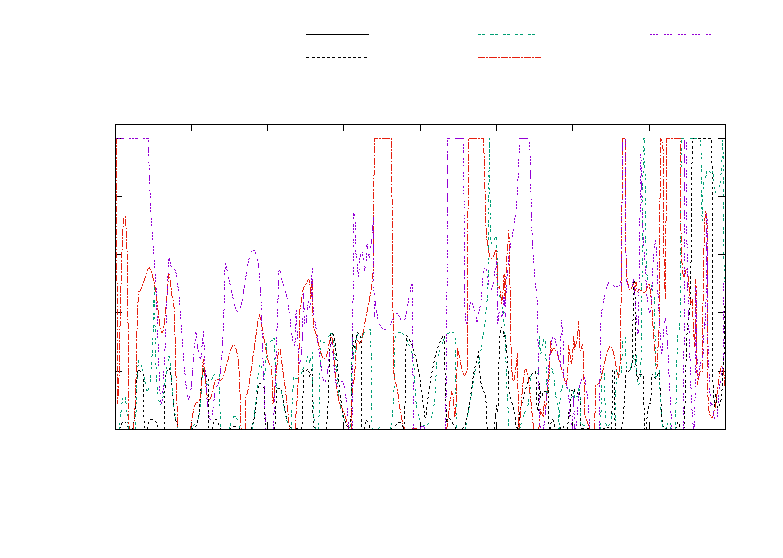
\includegraphics[width={360.00bp},height={252.00bp}]{MR-revise}}%
    \gplfronttext
  \end{picture}%
\endgroup
}
    \resizebox{0.45\textwidth}{!}{% GNUPLOT: LaTeX picture with Postscript
\begingroup
  % Encoding inside the plot.  In the header of your document, this encoding
  % should to defined, e.g., by using
  % \usepackage[cp1252,<other encodings>]{inputenc}
  % \inputencoding{cp1252}%s
  \makeatletter
  \providecommand\color[2][]{%
    \GenericError{(gnuplot) \space\space\space\@spaces}{%
      Package color not loaded in conjunction with
      terminal option `colourtext'%
    }{See the gnuplot documentation for explanation.%
    }{Either use 'blacktext' in gnuplot or load the package
      color.sty in LaTeX.}%
    \renewcommand\color[2][]{}%
  }%
  \providecommand\includegraphics[2][]{%
    \GenericError{(gnuplot) \space\space\space\@spaces}{%
      Package graphicx or graphics not loaded%
    }{See the gnuplot documentation for explanation.%
    }{The gnuplot epslatex terminal needs graphicx.sty or graphics.sty.}%
    \renewcommand\includegraphics[2][]{}%
  }%
  \providecommand\rotatebox[2]{#2}%
  \@ifundefined{ifGPcolor}{%
    \newif\ifGPcolor
    \GPcolorfalse
  }{}%
  \@ifundefined{ifGPblacktext}{%
    \newif\ifGPblacktext
    \GPblacktexttrue
  }{}%
  % define a \g@addto@macro without @ in the name:
  \let\gplgaddtomacro\g@addto@macro
  % define empty templates for all commands taking text:
  \gdef\gplbacktext{}%
  \gdef\gplfronttext{}%
  \makeatother
  \ifGPblacktext
    % no textcolor at all
    \def\colorrgb#1{}%
    \def\colorgray#1{}%
  \else
    % gray or color?
    \ifGPcolor
      \def\colorrgb#1{\color[rgb]{#1}}%
      \def\colorgray#1{\color[gray]{#1}}%
      \expandafter\def\csname LTw\endcsname{\color{white}}%
      \expandafter\def\csname LTb\endcsname{\color{black}}%
      \expandafter\def\csname LTa\endcsname{\color{black}}%
      \expandafter\def\csname LT0\endcsname{\color[rgb]{1,0,0}}%
      \expandafter\def\csname LT1\endcsname{\color[rgb]{0,1,0}}%
      \expandafter\def\csname LT2\endcsname{\color[rgb]{0,0,1}}%
      \expandafter\def\csname LT3\endcsname{\color[rgb]{1,0,1}}%
      \expandafter\def\csname LT4\endcsname{\color[rgb]{0,1,1}}%
      \expandafter\def\csname LT5\endcsname{\color[rgb]{1,1,0}}%
      \expandafter\def\csname LT6\endcsname{\color[rgb]{0,0,0}}%
      \expandafter\def\csname LT7\endcsname{\color[rgb]{1,0.3,0}}%
      \expandafter\def\csname LT8\endcsname{\color[rgb]{0.5,0.5,0.5}}%
    \else
      % gray
      \def\colorrgb#1{\color{black}}%
      \def\colorgray#1{\color[gray]{#1}}%
      \expandafter\def\csname LTw\endcsname{\color{white}}%
      \expandafter\def\csname LTb\endcsname{\color{black}}%
      \expandafter\def\csname LTa\endcsname{\color{black}}%
      \expandafter\def\csname LT0\endcsname{\color{black}}%
      \expandafter\def\csname LT1\endcsname{\color{black}}%
      \expandafter\def\csname LT2\endcsname{\color{black}}%
      \expandafter\def\csname LT3\endcsname{\color{black}}%
      \expandafter\def\csname LT4\endcsname{\color{black}}%
      \expandafter\def\csname LT5\endcsname{\color{black}}%
      \expandafter\def\csname LT6\endcsname{\color{black}}%
      \expandafter\def\csname LT7\endcsname{\color{black}}%
      \expandafter\def\csname LT8\endcsname{\color{black}}%
    \fi
  \fi
    \setlength{\unitlength}{0.0500bp}%
    \ifx\gptboxheight\undefined%
      \newlength{\gptboxheight}%
      \newlength{\gptboxwidth}%
      \newsavebox{\gptboxtext}%
    \fi%
    \setlength{\fboxrule}{0.5pt}%
    \setlength{\fboxsep}{1pt}%
\begin{picture}(7200.00,5040.00)%
    \gplgaddtomacro\gplbacktext{%
      \csname LTb\endcsname%%
      \put(1400,4600){\makebox(0,0)[r]{\strut{}$B$}}%
      \put(814,1077){\makebox(0,0)[r]{\strut{}$0$}}%
      \put(814,1635){\makebox(0,0)[r]{\strut{}$0.2$}}%
      \put(814,2193){\makebox(0,0)[r]{\strut{}$0.4$}}%
      \put(814,2751){\makebox(0,0)[r]{\strut{}$0.6$}}%
      \put(814,3309){\makebox(0,0)[r]{\strut{}$0.8$}}%
      \put(814,3867){\makebox(0,0)[r]{\strut{}$1$}}%
      \put(946,857){\makebox(0,0){\strut{}$-4$}}%
      \put(1678,857){\makebox(0,0){\strut{}$-3$}}%
      \put(2410,857){\makebox(0,0){\strut{}$-2$}}%
      \put(3142,857){\makebox(0,0){\strut{}$-1$}}%
      \put(3875,857){\makebox(0,0){\strut{}$0$}}%
      \put(4607,857){\makebox(0,0){\strut{}$1$}}%
      \put(5339,857){\makebox(0,0){\strut{}$2$}}%
      \put(6071,857){\makebox(0,0){\strut{}$3$}}%
      \put(6803,857){\makebox(0,0){\strut{}$4$}}%
    }%
    \gplgaddtomacro\gplfronttext{%
      \csname LTb\endcsname%%
      \put(209,2541){\rotatebox{-270}{\makebox(0,0){\strut{}MR}}}%
      \put(3874,527){\makebox(0,0){\strut{}$E(eV)$}}%
      \csname LTb\endcsname%%
      \put(2654,4867){\makebox(0,0)[r]{\strut{}$M=0$}}%
      \csname LTb\endcsname%%
      \put(2654,4647){\makebox(0,0)[r]{\strut{}$M=0.05$}}%
      \csname LTb\endcsname%%
      \put(4301,4867){\makebox(0,0)[r]{\strut{}$M=0.1$}}%
      \csname LTb\endcsname%%
      \put(4301,4647){\makebox(0,0)[r]{\strut{}$M=0.2$}}%
      \csname LTb\endcsname%%
      \put(5948,4867){\makebox(0,0)[r]{\strut{}$M=0.3$}}%
    }%
    \gplbacktext
    \put(0,0){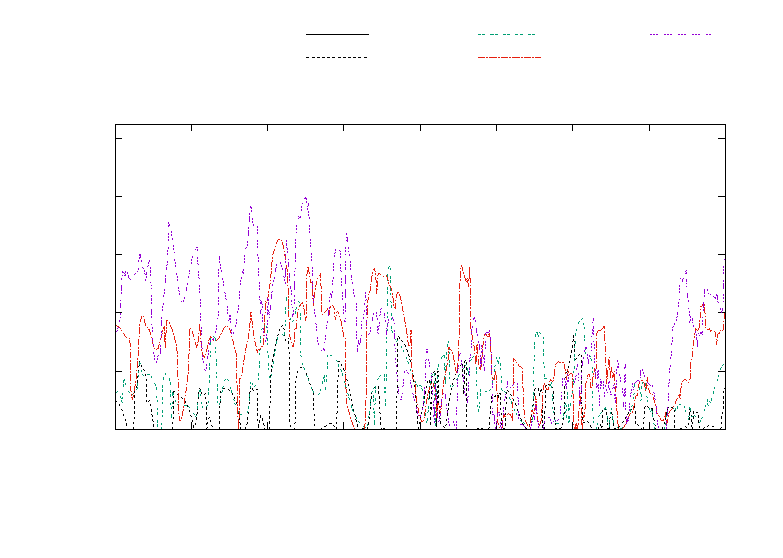
\includegraphics[width={360.00bp},height={252.00bp}]{MR_zig-revise}}%
    \gplfronttext
  \end{picture}%
\endgroup
}
  \end{latin}
\caption{مقاومت مغناطیس (MR) $\beta_{12}$-بوروفن در آرمچیر راحتی و لبه‌های زیگزاگی.}
\label{fig:MR}
\end{figure*}

\begin{figure*}[!ht]
  \begin{latin}
    \centering
    \resizebox{0.45\textwidth}{!}{% GNUPLOT: LaTeX picture with Postscript
\begin{latin}
\begingroup
  % Encoding inside the plot.  In the header of your document, this encoding
  % should to defined, e.g., by using
  % \usepackage[cp1252,<other encodings>]{inputenc}
  % \inputencoding{cp1252}%
  \makeatletter
  \providecommand\color[2][]{%
    \GenericError{(gnuplot) \space\space\space\@spaces}{%
      Package color not loaded in conjunction with
      terminal option `colourtext'%
    }{See the gnuplot documentation for explanation.%
    }{Either use 'blacktext' in gnuplot or load the package
      color.sty in LaTeX.}%
    \renewcommand\color[2][]{}%
  }%
  \providecommand\includegraphics[2][]{%
    \GenericError{(gnuplot) \space\space\space\@spaces}{%
      Package graphicx or graphics not loaded%
    }{See the gnuplot documentation for explanation.%
    }{The gnuplot epslatex terminal needs graphicx.sty or graphics.sty.}%
    \renewcommand\includegraphics[2][]{}%
  }%
  \providecommand\rotatebox[2]{#2}%
  \@ifundefined{ifGPcolor}{%
    \newif\ifGPcolor
    \GPcolorfalse
  }{}%
  \@ifundefined{ifGPblacktext}{%
    \newif\ifGPblacktext
    \GPblacktexttrue
  }{}%
  % define a \g@addto@macro without @ in the name:
  \let\gplgaddtomacro\g@addto@macro
  % define empty templates for all commands taking text:
  \gdef\gplbacktext{}%
  \gdef\gplfronttext{}%
  \makeatother
  \ifGPblacktext
    % no textcolor at all
    \def\colorrgb#1{}%
    \def\colorgray#1{}%
  \else
    % gray or color?
    \ifGPcolor
      \def\colorrgb#1{\color[rgb]{#1}}%
      \def\colorgray#1{\color[gray]{#1}}%
      \expandafter\def\csname LTw\endcsname{\color{white}}%
      \expandafter\def\csname LTb\endcsname{\color{black}}%
      \expandafter\def\csname LTa\endcsname{\color{black}}%
      \expandafter\def\csname LT0\endcsname{\color[rgb]{1,0,0}}%
      \expandafter\def\csname LT1\endcsname{\color[rgb]{0,1,0}}%
      \expandafter\def\csname LT2\endcsname{\color[rgb]{0,0,1}}%
      \expandafter\def\csname LT3\endcsname{\color[rgb]{1,0,1}}%
      \expandafter\def\csname LT4\endcsname{\color[rgb]{0,1,1}}%
      \expandafter\def\csname LT5\endcsname{\color[rgb]{1,1,0}}%
      \expandafter\def\csname LT6\endcsname{\color[rgb]{0,0,0}}%
      \expandafter\def\csname LT7\endcsname{\color[rgb]{1,0.3,0}}%
      \expandafter\def\csname LT8\endcsname{\color[rgb]{0.5,0.5,0.5}}%
    \else
      % gray
      \def\colorrgb#1{\color{black}}%
      \def\colorgray#1{\color[gray]{#1}}%
      \expandafter\def\csname LTw\endcsname{\color{white}}%
      \expandafter\def\csname LTb\endcsname{\color{black}}%
      \expandafter\def\csname LTa\endcsname{\color{black}}%
      \expandafter\def\csname LT0\endcsname{\color{black}}%
      \expandafter\def\csname LT1\endcsname{\color{black}}%
      \expandafter\def\csname LT2\endcsname{\color{black}}%
      \expandafter\def\csname LT3\endcsname{\color{black}}%
      \expandafter\def\csname LT4\endcsname{\color{black}}%
      \expandafter\def\csname LT5\endcsname{\color{black}}%
      \expandafter\def\csname LT6\endcsname{\color{black}}%
      \expandafter\def\csname LT7\endcsname{\color{black}}%
      \expandafter\def\csname LT8\endcsname{\color{black}}%
    \fi
  \fi
    \setlength{\unitlength}{0.0500bp}%
    \ifx\gptboxheight\undefined%
      \newlength{\gptboxheight}%
      \newlength{\gptboxwidth}%
      \newsavebox{\gptboxtext}%
    \fi%
    \setlength{\fboxrule}{0.5pt}%
    \setlength{\fboxsep}{1pt}%
\begin{picture}(7200.00,5040.00)%
    \gplgaddtomacro\gplbacktext{%
      \csname LTb\endcsname%%
      \put(1300,4200){\makebox(0,0)[r]{\strut{}$A$}}%
      \put(946,704){\makebox(0,0)[r]{\strut{}$-0.3$}}%
      \put(946,1323){\makebox(0,0)[r]{\strut{}$-0.2$}}%
      \put(946,1942){\makebox(0,0)[r]{\strut{}$-0.1$}}%
      \put(946,2562){\makebox(0,0)[r]{\strut{}$0$}}%
      \put(946,3181){\makebox(0,0)[r]{\strut{}$0.1$}}%
      \put(946,3800){\makebox(0,0)[r]{\strut{}$0.2$}}%
      \put(946,4419){\makebox(0,0)[r]{\strut{}$0.3$}}%
      \put(1078,484){\makebox(0,0){\strut{}$0$}}%
      \put(2509,484){\makebox(0,0){\strut{}$0.5$}}%
      \put(3941,484){\makebox(0,0){\strut{}$1$}}%
      \put(5372,484){\makebox(0,0){\strut{}$1.5$}}%
      \put(6803,484){\makebox(0,0){\strut{}$2$}}%
    }%
    \gplgaddtomacro\gplfronttext{%
      \csname LTb\endcsname%%
      \put(209,2561){\rotatebox{-270}{\makebox(0,0){\strut{}$\tau/V$}}}%
      \put(3940,154){\makebox(0,0){\strut{}$\theta$}}%
      \csname LTb\endcsname%%
      \put(5816,4246){\makebox(0,0)[r]{\strut{}$M=0.05$}}%
      \csname LTb\endcsname%%
      \put(5816,4026){\makebox(0,0)[r]{\strut{}$M=0.10$}}%
      \csname LTb\endcsname%%
      \put(5816,3806){\makebox(0,0)[r]{\strut{}$M=0.20$}}%
      \csname LTb\endcsname%%
      \put(5816,3586){\makebox(0,0)[r]{\strut{}$M=0.30$}}%
      \csname LTb\endcsname%%
      \put(3940,4709){\makebox(0,0){\strut{}Spin Torque 2D}}%
    }%
    \gplbacktext
    \put(0,0){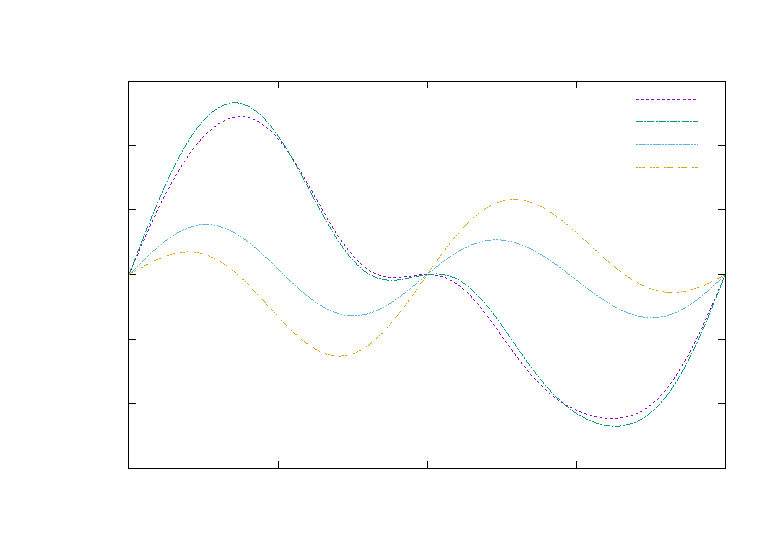
\includegraphics[width={360.00bp},height={252.00bp}]{stt}}%
    \gplfronttext
  \end{picture}%
\endgroup
\end{latin}}
    \resizebox{0.45\textwidth}{!}{% GNUPLOT: LaTeX picture with Postscript
\begingroup
  % Encoding inside the plot.  In the header of your document, this encoding
  % should to defined, e.g., by using
  % \usepackage[cp1252,<other encodings>]{inputenc}
  % \inputencoding{cp1252}%
  \makeatletter
  \providecommand\color[2][]{%
    \GenericError{(gnuplot) \space\space\space\@spaces}{%
      Package color not loaded in conjunction with
      terminal option `colourtext'%
    }{See the gnuplot documentation for explanation.%
    }{Either use 'blacktext' in gnuplot or load the package
      color.sty in LaTeX.}%
    \renewcommand\color[2][]{}%
  }%
  \providecommand\includegraphics[2][]{%
    \GenericError{(gnuplot) \space\space\space\@spaces}{%
      Package graphicx or graphics not loaded%
    }{See the gnuplot documentation for explanation.%
    }{The gnuplot epslatex terminal needs graphicx.sty or graphics.sty.}%
    \renewcommand\includegraphics[2][]{}%
  }%
  \providecommand\rotatebox[2]{#2}%
  \@ifundefined{ifGPcolor}{%
    \newif\ifGPcolor
    \GPcolorfalse
  }{}%
  \@ifundefined{ifGPblacktext}{%
    \newif\ifGPblacktext
    \GPblacktexttrue
  }{}%
  % define a \g@addto@macro without @ in the name:
  \let\gplgaddtomacro\g@addto@macro
  % define empty templates for all commands taking text:
  \gdef\gplbacktext{}%
  \gdef\gplfronttext{}%
  \makeatother
  \ifGPblacktext
    % no textcolor at all
    \def\colorrgb#1{}%
    \def\colorgray#1{}%
  \else
    % gray or color?
    \ifGPcolor
      \def\colorrgb#1{\color[rgb]{#1}}%
      \def\colorgray#1{\color[gray]{#1}}%
      \expandafter\def\csname LTw\endcsname{\color{white}}%
      \expandafter\def\csname LTb\endcsname{\color{black}}%
      \expandafter\def\csname LTa\endcsname{\color{black}}%
      \expandafter\def\csname LT0\endcsname{\color[rgb]{1,0,0}}%
      \expandafter\def\csname LT1\endcsname{\color[rgb]{0,1,0}}%
      \expandafter\def\csname LT2\endcsname{\color[rgb]{0,0,1}}%
      \expandafter\def\csname LT3\endcsname{\color[rgb]{1,0,1}}%
      \expandafter\def\csname LT4\endcsname{\color[rgb]{0,1,1}}%
      \expandafter\def\csname LT5\endcsname{\color[rgb]{1,1,0}}%
      \expandafter\def\csname LT6\endcsname{\color[rgb]{0,0,0}}%
      \expandafter\def\csname LT7\endcsname{\color[rgb]{1,0.3,0}}%
      \expandafter\def\csname LT8\endcsname{\color[rgb]{0.5,0.5,0.5}}%
    \else
      % gray
      \def\colorrgb#1{\color{black}}%
      \def\colorgray#1{\color[gray]{#1}}%
      \expandafter\def\csname LTw\endcsname{\color{white}}%
      \expandafter\def\csname LTb\endcsname{\color{black}}%
      \expandafter\def\csname LTa\endcsname{\color{black}}%
      \expandafter\def\csname LT0\endcsname{\color{black}}%
      \expandafter\def\csname LT1\endcsname{\color{black}}%
      \expandafter\def\csname LT2\endcsname{\color{black}}%
      \expandafter\def\csname LT3\endcsname{\color{black}}%
      \expandafter\def\csname LT4\endcsname{\color{black}}%
      \expandafter\def\csname LT5\endcsname{\color{black}}%
      \expandafter\def\csname LT6\endcsname{\color{black}}%
      \expandafter\def\csname LT7\endcsname{\color{black}}%
      \expandafter\def\csname LT8\endcsname{\color{black}}%
    \fi
  \fi
    \setlength{\unitlength}{0.0500bp}%
    \ifx\gptboxheight\undefined%
      \newlength{\gptboxheight}%
      \newlength{\gptboxwidth}%
      \newsavebox{\gptboxtext}%
    \fi%
    \setlength{\fboxrule}{0.5pt}%
    \setlength{\fboxsep}{1pt}%
\begin{picture}(7200.00,5040.00)%
    \gplgaddtomacro\gplbacktext{%
    }%
    \gplgaddtomacro\gplfronttext{%
      \csname LTb\endcsname%%
      \put(1300,3900){\makebox(0,0)[r]{\strut{}$B$}}%
      \put(936,674){\makebox(0,0){\strut{}$-4$}}%
      \put(1602,674){\makebox(0,0){\strut{}$-3$}}%
      \put(2268,674){\makebox(0,0){\strut{}$-2$}}%
      \put(2934,674){\makebox(0,0){\strut{}$-1$}}%
      \put(3600,674){\makebox(0,0){\strut{}$0$}}%
      \put(4266,674){\makebox(0,0){\strut{}$1$}}%
      \put(4932,674){\makebox(0,0){\strut{}$2$}}%
      \put(5598,674){\makebox(0,0){\strut{}$3$}}%
      \put(6264,674){\makebox(0,0){\strut{}$4$}}%
      \put(3600,344){\makebox(0,0){\strut{}$E(eV)$}}%
      \put(693,917){\makebox(0,0)[r]{\strut{}$-6$}}%
      \put(693,1318){\makebox(0,0)[r]{\strut{}$-4$}}%
      \put(693,1719){\makebox(0,0)[r]{\strut{}$-2$}}%
      \put(693,2120){\makebox(0,0)[r]{\strut{}$0$}}%
      \put(693,2520){\makebox(0,0)[r]{\strut{}$2$}}%
      \put(693,2920){\makebox(0,0)[r]{\strut{}$4$}}%
      \put(693,3321){\makebox(0,0)[r]{\strut{}$6$}}%
      \put(693,3722){\makebox(0,0)[r]{\strut{}$8$}}%
      \put(693,4123){\makebox(0,0)[r]{\strut{}$10$}}%
      \put(363,2520){\rotatebox{-270}{\makebox(0,0){\strut{}$\tau$}}}%
      \put(6795,917){\makebox(0,0)[l]{\strut{}$0$}}%
      \put(6795,1237){\makebox(0,0)[l]{\strut{}$0.2$}}%
      \put(6795,1558){\makebox(0,0)[l]{\strut{}$0.4$}}%
      \put(6795,1878){\makebox(0,0)[l]{\strut{}$0.6$}}%
      \put(6795,2199){\makebox(0,0)[l]{\strut{}$0.8$}}%
      \put(6795,2520){\makebox(0,0)[l]{\strut{}$1$}}%
      \put(6795,2840){\makebox(0,0)[l]{\strut{}$1.2$}}%
      \put(6795,3161){\makebox(0,0)[l]{\strut{}$1.4$}}%
      \put(6795,3481){\makebox(0,0)[l]{\strut{}$1.6$}}%
      \put(6795,3802){\makebox(0,0)[l]{\strut{}$1.8$}}%
      \put(6795,4123){\makebox(0,0)[l]{\strut{}$2$}}%
      \put(7257,2520){\rotatebox{-270}{\makebox(0,0){\strut{}$\theta$}}}%
      \put(3600,4453){\makebox(0,0){\strut{}$M=0.1$}}%
    }%
    \gplbacktext
    \put(0,0){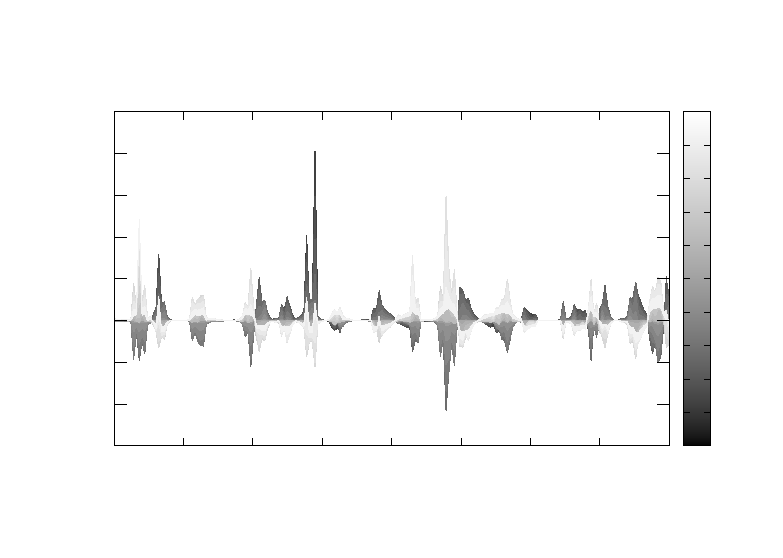
\includegraphics[width={360.00bp},height={252.00bp}]{stt-energy3d-0.1}}%
    \gplfronttext
  \end{picture}%
\endgroup
}
    \resizebox{0.45\textwidth}{!}{% GNUPLOT: LaTeX picture with Postscript
\begingroup
  % Encoding inside the plot.  In the header of your document, this encoding
  % should to defined, e.g., by using
  % \usepackage[cp1252,<other encodings>]{inputenc}
  % \inputencoding{cp1252}%
  \makeatletter
  \providecommand\color[2][]{%
    \GenericError{(gnuplot) \space\space\space\@spaces}{%
      Package color not loaded in conjunction with
      terminal option `colourtext'%
    }{See the gnuplot documentation for explanation.%
    }{Either use 'blacktext' in gnuplot or load the package
      color.sty in LaTeX.}%
    \renewcommand\color[2][]{}%
  }%
  \providecommand\includegraphics[2][]{%
    \GenericError{(gnuplot) \space\space\space\@spaces}{%
      Package graphicx or graphics not loaded%
    }{See the gnuplot documentation for explanation.%
    }{The gnuplot epslatex terminal needs graphicx.sty or graphics.sty.}%
    \renewcommand\includegraphics[2][]{}%
  }%
  \providecommand\rotatebox[2]{#2}%
  \@ifundefined{ifGPcolor}{%
    \newif\ifGPcolor
    \GPcolorfalse
  }{}%
  \@ifundefined{ifGPblacktext}{%
    \newif\ifGPblacktext
    \GPblacktexttrue
  }{}%
  % define a \g@addto@macro without @ in the name:
  \let\gplgaddtomacro\g@addto@macro
  % define empty templates for all commands taking text:
  \gdef\gplbacktext{}%
  \gdef\gplfronttext{}%
  \makeatother
  \ifGPblacktext
    % no textcolor at all
    \def\colorrgb#1{}%
    \def\colorgray#1{}%
  \else
    % gray or color?
    \ifGPcolor
      \def\colorrgb#1{\color[rgb]{#1}}%
      \def\colorgray#1{\color[gray]{#1}}%
      \expandafter\def\csname LTw\endcsname{\color{white}}%
      \expandafter\def\csname LTb\endcsname{\color{black}}%
      \expandafter\def\csname LTa\endcsname{\color{black}}%
      \expandafter\def\csname LT0\endcsname{\color[rgb]{1,0,0}}%
      \expandafter\def\csname LT1\endcsname{\color[rgb]{0,1,0}}%
      \expandafter\def\csname LT2\endcsname{\color[rgb]{0,0,1}}%
      \expandafter\def\csname LT3\endcsname{\color[rgb]{1,0,1}}%
      \expandafter\def\csname LT4\endcsname{\color[rgb]{0,1,1}}%
      \expandafter\def\csname LT5\endcsname{\color[rgb]{1,1,0}}%
      \expandafter\def\csname LT6\endcsname{\color[rgb]{0,0,0}}%
      \expandafter\def\csname LT7\endcsname{\color[rgb]{1,0.3,0}}%
      \expandafter\def\csname LT8\endcsname{\color[rgb]{0.5,0.5,0.5}}%
    \else
      % gray
      \def\colorrgb#1{\color{black}}%
      \def\colorgray#1{\color[gray]{#1}}%
      \expandafter\def\csname LTw\endcsname{\color{white}}%
      \expandafter\def\csname LTb\endcsname{\color{black}}%
      \expandafter\def\csname LTa\endcsname{\color{black}}%
      \expandafter\def\csname LT0\endcsname{\color{black}}%
      \expandafter\def\csname LT1\endcsname{\color{black}}%
      \expandafter\def\csname LT2\endcsname{\color{black}}%
      \expandafter\def\csname LT3\endcsname{\color{black}}%
      \expandafter\def\csname LT4\endcsname{\color{black}}%
      \expandafter\def\csname LT5\endcsname{\color{black}}%
      \expandafter\def\csname LT6\endcsname{\color{black}}%
      \expandafter\def\csname LT7\endcsname{\color{black}}%
      \expandafter\def\csname LT8\endcsname{\color{black}}%
    \fi
  \fi
    \setlength{\unitlength}{0.0500bp}%
    \ifx\gptboxheight\undefined%
      \newlength{\gptboxheight}%
      \newlength{\gptboxwidth}%
      \newsavebox{\gptboxtext}%
    \fi%
    \setlength{\fboxrule}{0.5pt}%
    \setlength{\fboxsep}{1pt}%
\begin{picture}(7200.00,5040.00)%
    \gplgaddtomacro\gplbacktext{%
    }%
    \gplgaddtomacro\gplfronttext{%
      \csname LTb\endcsname%%
      \put(1300,3900){\makebox(0,0)[r]{\strut{}$C$}}%
      \put(936,674){\makebox(0,0){\strut{}$-4$}}%
      \put(1602,674){\makebox(0,0){\strut{}$-3$}}%
      \put(2268,674){\makebox(0,0){\strut{}$-2$}}%
      \put(2934,674){\makebox(0,0){\strut{}$-1$}}%
      \put(3600,674){\makebox(0,0){\strut{}$0$}}%
      \put(4266,674){\makebox(0,0){\strut{}$1$}}%
      \put(4932,674){\makebox(0,0){\strut{}$2$}}%
      \put(5598,674){\makebox(0,0){\strut{}$3$}}%
      \put(6264,674){\makebox(0,0){\strut{}$4$}}%
      \put(3600,344){\makebox(0,0){\strut{}$E(eV)$}}%
      \put(693,917){\makebox(0,0)[r]{\strut{}$-4$}}%
      \put(693,1375){\makebox(0,0)[r]{\strut{}$-2$}}%
      \put(693,1833){\makebox(0,0)[r]{\strut{}$0$}}%
      \put(693,2291){\makebox(0,0)[r]{\strut{}$2$}}%
      \put(693,2749){\makebox(0,0)[r]{\strut{}$4$}}%
      \put(693,3207){\makebox(0,0)[r]{\strut{}$6$}}%
      \put(693,3665){\makebox(0,0)[r]{\strut{}$8$}}%
      \put(693,4123){\makebox(0,0)[r]{\strut{}$10$}}%
      \put(363,2520){\rotatebox{-270}{\makebox(0,0){\strut{}$\tau$}}}%
      \put(6795,917){\makebox(0,0)[l]{\strut{}$0$}}%
      \put(6795,1237){\makebox(0,0)[l]{\strut{}$0.2$}}%
      \put(6795,1558){\makebox(0,0)[l]{\strut{}$0.4$}}%
      \put(6795,1878){\makebox(0,0)[l]{\strut{}$0.6$}}%
      \put(6795,2199){\makebox(0,0)[l]{\strut{}$0.8$}}%
      \put(6795,2520){\makebox(0,0)[l]{\strut{}$1$}}%
      \put(6795,2840){\makebox(0,0)[l]{\strut{}$1.2$}}%
      \put(6795,3161){\makebox(0,0)[l]{\strut{}$1.4$}}%
      \put(6795,3481){\makebox(0,0)[l]{\strut{}$1.6$}}%
      \put(6795,3802){\makebox(0,0)[l]{\strut{}$1.8$}}%
      \put(6795,4123){\makebox(0,0)[l]{\strut{}$2$}}%
      \put(7257,2520){\rotatebox{-270}{\makebox(0,0){\strut{}$\theta$}}}%
      \put(3600,4453){\makebox(0,0){\strut{}$M=0.2$}}%
    }%
    \gplbacktext
    \put(0,0){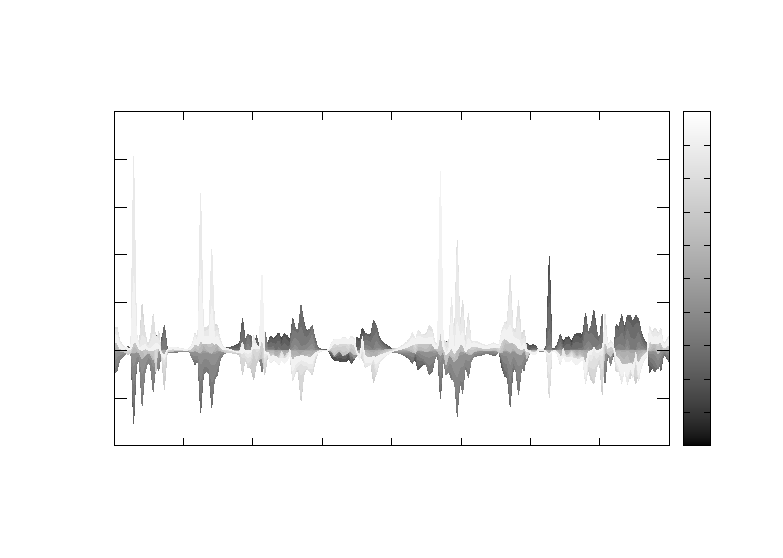
\includegraphics[width={360.00bp},height={252.00bp}]{stt-energy3d-0.2}}%
    \gplfronttext
  \end{picture}%
\endgroup
}
    \resizebox{0.45\textwidth}{!}{% GNUPLOT: LaTeX picture with Postscript
\begingroup
  % Encoding inside the plot.  In the header of your document, this encoding
  % should to defined, e.g., by using
  % \usepackage[cp1252,<other encodings>]{inputenc}
  % \inputencoding{cp1252}%
  \makeatletter
  \providecommand\color[2][]{%
    \GenericError{(gnuplot) \space\space\space\@spaces}{%
      Package color not loaded in conjunction with
      terminal option `colourtext'%
    }{See the gnuplot documentation for explanation.%
    }{Either use 'blacktext' in gnuplot or load the package
      color.sty in LaTeX.}%
    \renewcommand\color[2][]{}%
  }%
  \providecommand\includegraphics[2][]{%
    \GenericError{(gnuplot) \space\space\space\@spaces}{%
      Package graphicx or graphics not loaded%
    }{See the gnuplot documentation for explanation.%
    }{The gnuplot epslatex terminal needs graphicx.sty or graphics.sty.}%
    \renewcommand\includegraphics[2][]{}%
  }%
  \providecommand\rotatebox[2]{#2}%
  \@ifundefined{ifGPcolor}{%
    \newif\ifGPcolor
    \GPcolorfalse
  }{}%
  \@ifundefined{ifGPblacktext}{%
    \newif\ifGPblacktext
    \GPblacktexttrue
  }{}%
  % define a \g@addto@macro without @ in the name:
  \let\gplgaddtomacro\g@addto@macro
  % define empty templates for all commands taking text:
  \gdef\gplbacktext{}%
  \gdef\gplfronttext{}%
  \makeatother
  \ifGPblacktext
    % no textcolor at all
    \def\colorrgb#1{}%
    \def\colorgray#1{}%
  \else
    % gray or color?
    \ifGPcolor
      \def\colorrgb#1{\color[rgb]{#1}}%
      \def\colorgray#1{\color[gray]{#1}}%
      \expandafter\def\csname LTw\endcsname{\color{white}}%
      \expandafter\def\csname LTb\endcsname{\color{black}}%
      \expandafter\def\csname LTa\endcsname{\color{black}}%
      \expandafter\def\csname LT0\endcsname{\color[rgb]{1,0,0}}%
      \expandafter\def\csname LT1\endcsname{\color[rgb]{0,1,0}}%
      \expandafter\def\csname LT2\endcsname{\color[rgb]{0,0,1}}%
      \expandafter\def\csname LT3\endcsname{\color[rgb]{1,0,1}}%
      \expandafter\def\csname LT4\endcsname{\color[rgb]{0,1,1}}%
      \expandafter\def\csname LT5\endcsname{\color[rgb]{1,1,0}}%
      \expandafter\def\csname LT6\endcsname{\color[rgb]{0,0,0}}%
      \expandafter\def\csname LT7\endcsname{\color[rgb]{1,0.3,0}}%
      \expandafter\def\csname LT8\endcsname{\color[rgb]{0.5,0.5,0.5}}%
    \else
      % gray
      \def\colorrgb#1{\color{black}}%
      \def\colorgray#1{\color[gray]{#1}}%
      \expandafter\def\csname LTw\endcsname{\color{white}}%
      \expandafter\def\csname LTb\endcsname{\color{black}}%
      \expandafter\def\csname LTa\endcsname{\color{black}}%
      \expandafter\def\csname LT0\endcsname{\color{black}}%
      \expandafter\def\csname LT1\endcsname{\color{black}}%
      \expandafter\def\csname LT2\endcsname{\color{black}}%
      \expandafter\def\csname LT3\endcsname{\color{black}}%
      \expandafter\def\csname LT4\endcsname{\color{black}}%
      \expandafter\def\csname LT5\endcsname{\color{black}}%
      \expandafter\def\csname LT6\endcsname{\color{black}}%
      \expandafter\def\csname LT7\endcsname{\color{black}}%
      \expandafter\def\csname LT8\endcsname{\color{black}}%
    \fi
  \fi
    \setlength{\unitlength}{0.0500bp}%
    \ifx\gptboxheight\undefined%
      \newlength{\gptboxheight}%
      \newlength{\gptboxwidth}%
      \newsavebox{\gptboxtext}%
    \fi%
    \setlength{\fboxrule}{0.5pt}%
    \setlength{\fboxsep}{1pt}%
\begin{picture}(7200.00,5040.00)%
    \gplgaddtomacro\gplbacktext{%
    }%
    \gplgaddtomacro\gplfronttext{%
      \csname LTb\endcsname%%
      \put(1300,3900){\makebox(0,0)[r]{\strut{}$D$}}%
      \put(936,674){\makebox(0,0){\strut{}$-4$}}%
      \put(1602,674){\makebox(0,0){\strut{}$-3$}}%
      \put(2268,674){\makebox(0,0){\strut{}$-2$}}%
      \put(2934,674){\makebox(0,0){\strut{}$-1$}}%
      \put(3600,674){\makebox(0,0){\strut{}$0$}}%
      \put(4266,674){\makebox(0,0){\strut{}$1$}}%
      \put(4932,674){\makebox(0,0){\strut{}$2$}}%
      \put(5598,674){\makebox(0,0){\strut{}$3$}}%
      \put(6264,674){\makebox(0,0){\strut{}$4$}}%
      \put(3600,344){\makebox(0,0){\strut{}$E(eV)$}}%
      \put(693,917){\makebox(0,0)[r]{\strut{}$-6$}}%
      \put(693,1375){\makebox(0,0)[r]{\strut{}$-4$}}%
      \put(693,1833){\makebox(0,0)[r]{\strut{}$-2$}}%
      \put(693,2291){\makebox(0,0)[r]{\strut{}$0$}}%
      \put(693,2749){\makebox(0,0)[r]{\strut{}$2$}}%
      \put(693,3207){\makebox(0,0)[r]{\strut{}$4$}}%
      \put(693,3665){\makebox(0,0)[r]{\strut{}$6$}}%
      \put(693,4123){\makebox(0,0)[r]{\strut{}$8$}}%
      \put(363,2520){\rotatebox{-270}{\makebox(0,0){\strut{}$\tau$}}}%
      \put(6795,917){\makebox(0,0)[l]{\strut{}$0$}}%
      \put(6795,1237){\makebox(0,0)[l]{\strut{}$0.2$}}%
      \put(6795,1558){\makebox(0,0)[l]{\strut{}$0.4$}}%
      \put(6795,1878){\makebox(0,0)[l]{\strut{}$0.6$}}%
      \put(6795,2199){\makebox(0,0)[l]{\strut{}$0.8$}}%
      \put(6795,2520){\makebox(0,0)[l]{\strut{}$1$}}%
      \put(6795,2840){\makebox(0,0)[l]{\strut{}$1.2$}}%
      \put(6795,3161){\makebox(0,0)[l]{\strut{}$1.4$}}%
      \put(6795,3481){\makebox(0,0)[l]{\strut{}$1.6$}}%
      \put(6795,3802){\makebox(0,0)[l]{\strut{}$1.8$}}%
      \put(6795,4123){\makebox(0,0)[l]{\strut{}$2$}}%
      \put(7257,2520){\rotatebox{-270}{\makebox(0,0){\strut{}$\theta$}}}%
      \put(3600,4453){\makebox(0,0){\strut{}$M=0.3$}}%
    }%
    \gplbacktext
    \put(0,0){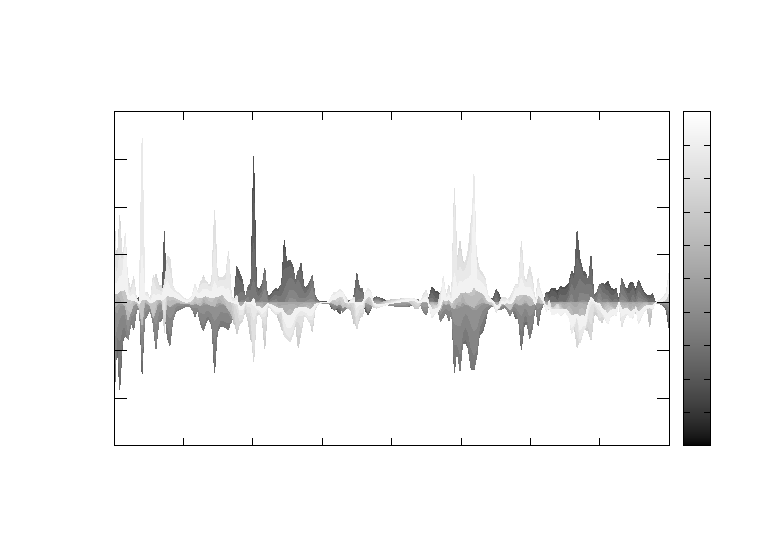
\includegraphics[width={360.00bp},height={252.00bp}]{stt-energy3d-0.3.eps}}%
    \gplfronttext
  \end{picture}%
\endgroup
}
  \end{latin}
    \caption{الف) گشتاور اسپینی از بوروفن با لبه آرمچیر، با عرض سلول 4 واحد، برای متغیر مغناطیسی لیدها با توجه به درجه نسبی در جهت z در \lr{E = 0 eV} ترسیم شده است. ب، ج، د) گشتاور اسپینی با مغناطش \lr{0.1، 0.2، 0.3 eV} نسبت به انرژی در تمام محدوده زوایای نسبی.}
    \label{fig:stt}
\end{figure*}

% \section{مقاله دوم}
% ترابرد وابسته به اسپین و گشتاور ترابرد اسپین در شیر اسپینی مبتنی بر بوروفن† عرفان نیکان، امیرحسین احمدخان کردبچه، b‡ 
\section{اسپینترونیک}
اسپینترونیک معمولاً به پدیده‌هایی اطلاق می‌شود که در آن اسپین الکترون‌ها در یک محیط حالت جامد نقش تعیین‌کننده را ایفا می‌کند. به معنای محدودتر اسپینترونیک یک زمینه تحقیقاتی نوظهور در الکترونیک است. دستگاه های اسپینترونیک بر اساس کنترل اسپین الکترون با کنترل الکتریکی و نوری اسپین یا مغناطیس هستند. در حالی که اسپینترونیک فلزی قبلاً جایگاه خود را در صنعت رایانه پیدا کرده است. سیستم‌های مقاومت مغناطیسی غول‌پیکر به عنوان هدهای خواندن دیسک استفاده می‌کنند، اسپینترونیک نیمه‌رسانا هنوز پتانسیل کامل خود را نشان نداده است. اساسی‌ترین برهمکنش وابسته به اسپین در نیمه هادی‌های غیر مغناطیسی، جفت شدن اسپین-مدار است. بسته به تقارن‌های کریستالی مواد، و همچنین ویژگی‌های ساختاری هتروساختارها مبتنی بر نیمه‌رسانا، کوپلینگ مداری اسپین شکل‌های عملکردی متفاوتی به خود می‌گیرد و زمین بازی خوبی از همیلتونی‌های مدار اسپینی موثر ایجاد می‌کند. هامیلتونی‌های مؤثر برای مرتبط‌ترین کلاس‌های مواد و ناهمساختارها در اینجا از توضیحات ساختار نوار الکترونیکی واقعی مشتق شده‌اند. 

اکثر سیستم های دستگاه‌های نیمه هادی هنوز مفاهیم نظری هستند و منتظر نمایش های تجربی هستند. مروری بر منتخب پیشنهادی، و چند دستگاه نشان‌داده‌شده، با شرح دقیق دو کلاس مهم ارائه می‌شود: ساختارهای تونلی تشدید مغناطیسی و دیودها و ترانزیستورهای مغناطیسی دوقطبی.

\section{رسانش کوانتومی اسپین}

در بوروفین $\beta_{12}$ فقط چند مورد محاسبات دریچه اسپینی برای ساختار \lr{CIP} انجام شده است. خلأ این محاسبات مختلف، از جمله رسانندگی \lr{P} و \lr{AP} و \lr{MR} و \lr{STT}، در ساختار \lr{CPP} دریچه اسپینی برای $\beta_{12}$بوروفن 74 احساس میشود. این رساله به بررسی تحلیل نظری ترابرد وابسته به اسپین و ترابرد گشتاور اسپین برای  ساختار اتصال \lr{FM/normal/FM} مبتنی بر بوروفن می‌پردازد.  این مطالعه بر روی نانوریبان‌های بوروفن \lr{(BNRs)} به عنوان مبنایی برای محاسبات عددی دریچه اسپینی برای رسانندگی در هر دو پیکربندی که بردارهای مغناطیسی لیدها موازی یا ضد موازی با یکدیگر هستند (به ترتیب پیکربندی‌های \lr{P} و \lr{AP})، مقاومت مغناطیسی \lr{(MR)} تمرکز میکند. و گشتاور ترابرد اسپین \lr{(STT)}. رویکردهای فرمالیسم \lr{Landauer} و تابع گرین غیرتعادلی \lr{(NEGF)} برای استخراج جریان های تونل زنی وابسته به اسپین در محل اتصال تونل مغناطیسی \lr{(MTJ)} استفاده می شود. در اینجا ابتدا رسانایی بوروفن برای هر دو پیکربندی \lr{P} و \lr{AP} محاسبه میشود و رسانایی صفر در برخی انرژی‌ها در پیکربندی \lr{AP} و رسانایی غیر صفر در پیکربندی \lr{P} مشاهده میشود. این ویژگی حالت های \lr{ON} و \lr{OFF} را برای استفاده در سوئیچ ایجاد می کند. ترکیب پراکندگی وابسته به اسپین و فیلتر انتخاب نوار ممکن است دلیل رسانایی صفر را با استفاده از پاریته زیر‌نوارها در پیکربندی \lr{AP} را توضیح دهد.نتایج محاسبات برای \lr{BNR} زیگزاگ نشان میدهد که رسانایی همیشه بزرگتر از $e^2/h$ برای پیکربندی \lr{P} مغناطیس‌های لید است. برای پیکربندی \lr{AP}، رسانایی در محدوده انرژی خاص صفر می شود. یک فلات \lr{MR} کامل برای اتصال در غیاب بی نظمی یافت می شود، که ثابت می کند کاندیدای عالی دریچه اسپینی است.تغییرات گشتاور ترابرد اسپین با انرژی فرمی و زاویه نسبی بین دو مغناطش الکترود در شدت های مغناطیسی فرومغناطیسی مختلف بررسی شده است. تغییرات \lr{STT} با انرژی فرمی و زاویه نسبی بین دو مغناطش الکترود، برای قدرت های مختلف مغناطش فرومغناطیسی مورد مطالعه قرار گرفته است. محاسبات نشان می دهد که ولتاژ بایاس \lr{STT} در واحد $(e/4\pi)$، به عنوان تابعی از انرژی فرمی، به طور قابل توجهی در نزدیکی انرژی نقطه دیراک کاهش می یابد. علاوه بر این، یک الگوی نوسانی سینوسی را می توان در \lr{STT} در ولتاژ بایاس واحد \lr{V} در مقابل زاویه بین دو مغناطش الکترود تشخیص داد که با افزایش \lr{M} تشدید می شود. در نهایت، به منظور درک صحیح سیستم، \lr{G} به عنوان تابعی از زاویه نسبی بین دو مغناطش الکترود، و همچنین در اطراف انرژی نقطه دیراک بررسی میشود.ولتاژ بایاس \lr{STT} بوروفن دارای خواص منحصر به فردی از جمله چگالی کم و سختی بالا، مقاومت در برابر حرارت و رسانایی الکتریکی است که آن را به یک نامزد امیدوارکننده برای اسپین ترونیک تبدیل می کند. این مقاله تجزیه و تحلیل جامعی از خواص بوروفن وابسته به اسپین و کاربردهای بالقوه آن در اسپینترونیک ارائه می دهد.

\section{دریچه اسپینی:}
یکی از پیشرفت‌های مهم در دو دهه اخیر، دریچه اسپینی  است، دستگاهی با دو اتصال مغناطیسی (شکل\ref{fig:spinvalve}) اگر در یک جهت مغناطیسی شوند (پیکربندی موازی، \lr{P})، مقاومت حاصل از مغناطیسی شدن آنها کمتر است. در جهت مخالف (پیکربندی پاد موازی، \lr{AP}). از زمان اولین نمایش خود در سال 1988، به سرعت به عنوان یک دستگاه خواندن برای درک اطلاعات ذخیره شده در یک حافظه مغناطیسی کاربرد پیدا کرد و این کشف با جایزه نوبل در سال 2007 شناخته شد.
\begin{figure*}[!ht]
  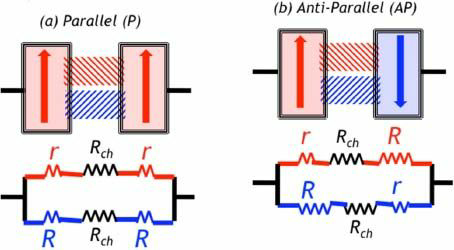
\includegraphics[width=1\linewidth]{./figures/spinvalve.png}
  \caption{دریچه اسپینی: (الف) پیکربندی موازی (P). (ب) پیکربندی ضد موازی (AP).}
  \label{fig:spinvalve}
\end{figure*}
تا اینجا ما فقط به اسپین به عنوان بخشی از "ضریب تبهگنی ، (\lr{g})" اشاره کرده‌ایم، ایده این است که حالت‌های الکترونیکی همیشه به صورت جفت می‌آیند که یکی مربوط به هر اسپین است. همانطور که در شکل\ref{fig:spinvalve} انجام دادیم، می‌توانیم اینها را «بالا» و «پایین» یا «چپ» و «راست» یا حتی «قرمز» و «آبی» بنامیم. توجه داشته باشید که این دو اسپین از نظر مکانی از هم جدا نیستند، حتی اگر کانال قرمز و آبی را برای وضوح از هم جدا کرد.

معمولاً دو کانال یکسان هستند و می توانیم رسانایی ناشی از یک را محاسبه کنیم و به یاد داشته باشیم که در دو ضرب کنیم. اما در دستگاه‌های دریچه اسپین،اتصال‌ها مغناطیده هستند که با دو کانال اسپین برخورد متفاوتی می‌کنند و عملکرد یک دریچه اسپینی با فرض اینکه که هر کانال اسپینی مقاومت رابط  متفاوتی، بسته به مغناطش اتصال، دارد،که یا موازی (اسپین اکثریت) یا پاد موازی (اسپین اقلیت) با مغناطش اتصال‌ها است.

اگر مقاومت رابط را برای اسپین های اکثریت r و برای اسپین های اقلیت R $(r < R)$ فرض کنیم، می توانیم نمایش های مدار ساده ای را برای پیکربندی های \lr{P} و \lr{AP} همانطور که نشان داده شده است ترسیم کنیم، با $R_{ch}$ نشان دهنده مقاومت کانال است. سپس تئوری مدارهای ابتدایی مقاومت پیکربندی موازی را به ما می دهد

همانطور که در شکل\ref{fig:model} نشان داده شده است، یک نانوروبان بوروفن غیر مغناطیسی \lr{(BNR)} با دو لید (به عنوان ناحیه مرکزی) که بین دو نانوروبان بوروفن \lr{FM} نیمه نامتناهی (به عنوان دو الکترود) قرار گرفته است، یک دستگاه شیر اسپینی را تشکیل می دهد. شایان ذکر است که حامل های بار بوروفن به طور کلی قطبش اسپینی نیستند و خاصیت مغناطیسی توسط یک بستر فرومغناطیسی عایق (با رشد بوروفن بر روی عایق \lr{FM}) به سرنخ های بوروفن تزریق می شود. از آنجایی که استفاده از میدان مغناطیسی می تواند برای شکستن تقارن معکوس زمانی مورد استفاده قرار گیرد، میدان تبادل ایجاد شده از طریق اثر مجاورت ناشی از یک بستر عایق فرومغناطیسی، باعث می شود که زمان معکوس یا تقارن اسپین شکسته شود. بر خلاف روشهای جایگزین برای شکستن \lr{TRS}، مانند دوپینگ 79،80 اتم فلزات واسطه و حجم‌دهی اتمی 81،82، این تکنیک یک دستکاری برهمکنش کوتاه برد خارجی است که تأثیری بر تحرک الکترون در کاربردهای الکترونیکی ندارد. اگر ناحیه هسته دارای طول \lr{L} و دارای \lr{N} اتم در عرض باشد، این ناحیه دارای $5 N (2L + 1)$ اتم است. مجموع هامیلتونی سیستم شیر اسپینی به صورت زیر بدست می آید:

\begin{equation}
  H= H_L + H_R + H_c + H_T,
\end{equation}
که
\begin{equation}
H_{L}=\sum\limits_{i\in L,\sigma }{\left( E_{L}+\sigma M_{L} \right)} a_{i\sigma }^{\dagger} a_{i\sigma }-\sum\limits_{i,i+\alpha \in L,\sigma}{\left( t_{\alpha } a_{i\sigma}^{\dagger} a_{i+\alpha \ \sigma }+H.c.\right)},
\end{equation}
\begin{equation}
\begin{split}
H_{R}=\sum_{i\in R,\sigma}{\left( E_{R}+\sigma M_{R} cos\phi M_{R}\sin \phi\right)} a_{i\sigma}^{\dagger} a_{i\sigma } \\
-\sum_{i\in R,\sigma} t_{\alpha } a_{i\sigma}^{\dagger} a_{i+\alpha\sigma}+H.c.,
\end{split}
\end{equation}
\begin{equation}
H_{C}=\sum_{i\in \ C,\sigma }{{{E}_{C}}}a_{i\sigma }^{\dagger}{{a}_{i\sigma }}-\sum_{i,i+\alpha \in \ C,\sigma }{({{t}_{\alpha }}\ a_{i}^{\dagger }{{a}_{i+\alpha }}+H.c.)},
\end{equation}
\begin{equation}
H_{T}=-\sum_{i\in \ C,i+\alpha \in L,R,\sigma}{{{t}_{\alpha }}}\ a_{i\sigma }^{\dagger }{{a}_{i+\alpha \ \sigma }}+H.c.,
\end{equation}

جایی که $E_L$، $E_R$ و $E_C$ به ترتیب انرژیهای موجود در نانوروبانهای بوروفن در لیدهای چپ و راست و ناحیه مرکزی هستند که میتوانند با ولتاژ گیت تنظیم شوند، بسته به محل نقطه شبکه، همانطور که در جدول\ref{tbl:hoppingtable} نشان داده شده است.

\begin{equation}
  \begin{aligned}
  & P:{{\left[ \frac{1}{2r+{{R}_{ch}}}+\frac{1}{2R+{{R}_{ch}}} \right]}^{-1}} \\ 
 & AP:\frac{r+R+{{R}_{ch}}}{2}  
  \end{aligned}
\end{equation}

\begin{figure*}
  \centering
  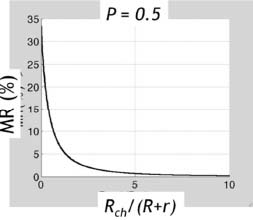
\includegraphics{./figures/MR-theory.png}
  \caption{تغییر در مقاومت مغناطیسی \lr{(MR)} به عنوان تابعی از مقاومت کانال نرمال شده است.}
  \label{fig:MRtheory}
\end{figure*}
ماهیت دستگاه دریچه اسپینی تفاوت بین $R_P$ و $R_{AP}$ %است و ما انتظار داریم زمانی که مقاومت کانال ناچیز است و همه چیز تحت سلطه رابط‌ها است، این موضوع بیشتر برجسته باشد. شکل\ref{fig:MRtheory} تغییر مقاومت مغناطیسی (\lr{MR}، تعریف شده در زیر) را به عنوان تابعی از مقاومت کانال (در هر اسپین) $R_{ch}$ نرمال شده به $r+R$ با فرض $P=0.5$ نشان می‌دهد. توجه داشته باشید که وقتی $R_{ch}$ نرمال شده بیش از مثلاً $~5$ افزایش یابد، \lr{MR} به سرعت از بین می رود.

استفاده از مواد دوبعدی، گرافن و سیلیسین، به عنوان پایه برای شیرهای اسپینی بسیار مورد توجه قرار گرفته است. بوروفن به عنوان یکی دیگر از مواد دوبعدی با خواص جدیدش کمتر برای این منظور مورد مطالعه قرار گرفته است. در این رساله از بوروفن نیز برای همین منظور استفاده خواهیم کرد. با توجه به کاربردهای عملی متعدد در دستگاه هایی مانند سوئیچ ها، هد هارد دیسک‌ها و \lr{MRAM}ها و همچنین \lr{STT-MRAM}‌ها و اهمیت پارامترهایی مانند رسانایی (موازی و ضد موازی)، \lr{MR} و \lr{STT} در طراحی یک شیر اسپینی، مطالعه این خواص در بوروفن مورد توجه قرار خواهد گرفت. نتیجه محاسبات عددی برای \lr{CPP} برای پیکربندی های موازی \lr{(P)} و ضد موازی \lr{(AP)} متشکل از یک نانوروبان با عرض چهار سلول واحد در شکل\ref{fig:model} نشان داده شده است. در تمام محاسبات، الکترودهای چپ و راست به عنوان یک کانال بوروفن با مغناطیسی برابر، به صورت $M_L = M_R = M$ در نظر گرفته می شوند. خاصیت مغناطیسی توسط یک بستر فرومغناطیسی عایق (با رشد بوروفن بر روی عایق \lr{FM}) به سرنخ های بوروفن تزریق می شود. زاویه $\theta$ جهت گیری کلی مغناطش لیدهای راست و چپ را نسبت به یکدیگر تعیین می کند، در حالی که حالت خاص $\theta = 0 (\pi)$ به ترتیب مغناطش موازی (یا ضد موازی) لیدهای چپ و راست را نشان می دهد.

محاسبات ما نشان می دهد که برخلاف \lr{ZBNR} ها، \lr{ABNR}ها رفتار نیمه هادی یا فلزی را بسته به عرض روبان $W$ از خود نشان می دهند، به طوری که برای عرض های بزرگتر از مقدار بحرانی \AA $W_c = 11.08$، 86 رسانایی غیر صفر را می توان یافت، در حالی که سیستم رفتار می کند. مانند یک نیمه هادی برای عرض های کوچکتر از $W_c$. حالت های لبه را می توان در شکاف انرژی نیمه هادی‌ها و همچنین شکاف نوار جایگزیده هادی‌ها مشاهده کرد. در نتیجه، حتی اگر معمولاً از نیمه هادی‌ها استفاده می شود، حالت های صفر را می توان در عرض های مشخص شده مناسب ایجاد کرد. اعمال میدان مغناطیسی تبادل درون صفحه ای باعث می شود هامیلتونین اسپین قطبی شده با عملگر اسپین \lr{S} جابجایی نداشته باشد و در این حالت اسپین الکترون دیگر ثابت حرکتی در سیستم نخواهد بود. این بدان معناست که حالت اسپین ممکن است در جهت انتقال تغییر کند. در واقع، در نتیجه برهمکنش اسپین الکترون با میدان مغناطیسی تبادل درون صفحه، چرخش اسپین رخ میدهد، به عنوان مثال، الکترونی که با حالت اسپین بالا وارد کانال میشود ممکن است کانال را به صورت اسپین پایین ترک کند. 

هنگامی که یک میدان مغناطیسی به دلیل وجود یک زیرلایه عایق فرومغناطیسی روی لیدها اعمال می شود، یک میدان مغناطیسی خارج از صفحه به شیرهای اسپین وارد می شود. با توجه به بررسی های ما، در این مورد، رسانایی نسبت به لیدهای غیر مغناطیسی تغییراتی را نشان می دهد. تجزیه و تحلیل دقیق این تغییرات برای درک آنها و دانستن منشأ آنها یک مسئله کلیدی برای طراحی شیرهای اسپین قابل اجرا و بهره برداری کامل از پتانسیل آنها است. 

% در نتیجه تغییر خواص مغناطیسی لیدها از حالت غیر مغناطیسی به مغناطیسی شده، تغییر در تعداد و عرض فلات‌ها ایجاد می شود. با این حال، با افزایش مغناطش در الکترودها، انحراف از ساختار پله مانند به وضوح مشاهده می شود. دلیل این امر را می توان بر اساس خروج برخی از سطوح انرژی از ترانس تشریح کرد.

در نتیجه تغییر خواص مغناطیسی لیدها از حالت غیر مغناطیسی به مغناطیسی شده، تغییر در تعداد و عرض فلات‌ها ایجاد می شود. با این حال، با افزایش مغناطش در الکترودها، انحراف از ساختار پله مانند به وضوح مشاهده می شود. دلیل این امر را می توان بر اساس خروج برخی از سطوح انرژی از پنجره انرژی ترابرد به دلیل جدا شدن سطوح انرژی در الکترودها به همراه حفظ پاریته زیرنوار انرژی به عنوان یکی از مکانیسم های دیگر مؤثر بر ترابرد بیان کرد. جداسازی اسپین ناشی از \gls{اثر زیمن}، ساختار نوار را تغییر می‌دهد و در یک پنجره انرژی، تعداد زیر‌نوارها در هر دو حالت لیدهای مغناطیسی و غیر مغناطیسی تغییر می‌کند. در ادامه، انحرافات رسانایی در لیدهای مغناطیسی شده را در مقایسه با غیر مغناطیسی شده توضیح می دهیم که نمودارها رسانایی برای مغناطیس های مختلف $M$ را نشان می دهند و آنها را با حالت $M = 0$ مقایسه می کنند.

یکی از تغییرات از الکترودهای غیر مغناطیسی به حالت مغناطیسی، تغییر در تعداد و عرض صفحات در نمودار رسانندگی است که با افزایش مغناطیسی رخ می دهد. فلات‌ها در نمودار ترابرد در محدوده انرژی دیده می شوند که تعداد زیر‌نوارهای درگیر در فرآیند ترابرد ثابت است و زمانی که تعداد زیر‌نوارها در هر انرژی تغییر می کند، رسانایی نیز تغییر می کند. بنابراین، عرض پلاتوها در نمودار رسانایی به تفاوت بین زیر‌نوارهای انرژی بستگی دارد. با توجه به پایه دو اتمی موادی مانند گرافن، سیلیسن و غیره، فرورفتگی زیر‌نوارها حتی زمانی که تعامل تبادلی در نظر گرفته شود، رخ نمی دهد. دو نوع فاصله بین نواری دیده می شود. اولی فاصله بین دو زیر‌نوار اسپینی با تراز مخالف یکسان است که برابر با $2M$ است و دیگری فاصله بین نوار اسپینی \lr{N - 1} و زیر‌نوار اسپینی \lr{N}امین است. در بوروفن، به دلیل وجود یک اتم اضافی که در مرکز شش ضلعی قرار دارد، سطح انرژی ناشی از برهمکنش تبادلی تورفتگی وجود دارد. به همین دلیل، تنوع فاصله بین زیر‌نوارها بسیار بیشتر از قبل است که با تنوع عرض پلاتوها همراه است و در رسانش شکل\ref{fig:conductance}(b) نیز تایید شده است. بنابراین، برهمکنش مبادله به دلیل تغییری که در فاصله بین نوار ایجاد می کند، الگوی رسانایی گام مانند را بیشتر تغییر می دهد. 

یکی از اولین انحرافاتی که در لیدهای مغناطیسی نشان داده شده در شکل\ref{fig:conductance}(a,b) در مقایسه با حالت غیر مغناطیسی یافت می شود، وجود مراحل یا نوسانات در رسانایی با مقادیر کوچکتر از $G_0 (G_0 = e^2/h)$ در هر پیکربندی است. . علت این پدیده عدم تطابق بین پاریته زیر‌نوارهای کانال و پاریته زیر‌نوارهای الکترودهایی است که مقدار تونل آنها در مقایسه با حالت غیر مغناطیسی کمتر از یک $G_0$ است. این بدان معنی است که علاوه بر تعداد زیر‌نوارها در آن پنجره انرژی، پاریته زیر‌نوارها نیز در فرآیندهای تونل زنی و ترابرد الکترون بسیار مهم است. این متعاقبا باعث ایجاد فلات هایی با مقادیر فرد (که می توان گفت دارای خواص نیمه فلزی هستند) یا مقادیر نیمه صحیح می شود. البته برخلاف گرافن، این نوع تونل زنی الکترونی که در گرافن فقط در $E_F\le M$ دیده می شود، در بوروفن در سراسر طیف انرژی دیده می شود.
در غیاب هر گونه تعاملی که نرخ تونل زنی را کاهش دهد، با توجه به سهم  $G_0$ با توجه به هر زیر‌نوار در پنجره انرژی (همانطور که در مورد P مشاهده می شود)، وجود هر فلات با ارتفاع $2G_0$ در نمودار هدایت، میزان کل تونل زنی در پنجره انرژی را نشان می دهد. در مورد \lr{AP}، سرعت کامل تونلزنی در دو موقعیت اتفاق نمیافتد:

1. وقتی دو زیر‌نوار مرتبط با دو الکترود پاریته مخالف دارند، علیرغم عدم وجود شکاف انرژی در ساختار نوار، رسانش صفر خواهد بود. در پیکربندی \lr{AP}، شماره گذاری نوارهای انرژی در الکترودهای چپ و راست با یکدیگر متفاوت است و پاریته نوارهای فرعی نیز مخالف است. یعنی زیر‌نوارهایی با اعداد یکسان در دو الکترود دارای پاریته مخالف هستند. در این صورت بر اساس قاعده انتخاب پاریته، تونل زنی ممنوع خواهد بود، یعنی در طول فرآیند تونل زنی، الکترون با پاریته زوج در الکترود چپ نمی تواند به الکترون با پاریته فرد در الکترود سمت راست تبدیل شود و بنابراین با وجود عدم وجود شکاف نوار، رسانایی صفر خواهد بود. (برای چنین الکترونی، حتی اگر شکاف نواری صفر باشد، رسانش باز هم صفر خواهد بود.) 

تعداد زیر‌نوارها به تعداد اتم های ابرسلول بستگی دارد و در غیاب میدان مغناطیسی، دارای اسپین دوگانه هستند. انحطاط در الکترودها، زمانی که بستر مغناطیسی یک میدان مغناطیسی به صفحه اعمال می کند، تقسیم سطوح انرژی رخ می دهد. بنابراین تعداد زیر‌نوارها دو برابر می شود. از سوی دیگر، می دانیم که زیر‌نوارها دارای تقارن پاریته به دلیل ساختار متقارن ماتریس $H_k$ هستند که به تعداد آنها بستگی دارد. یعنی زیر‌نوارهای 0، 2، 4 و . . . زوج هستند و زیر‌نوارهای 1، 3، 5 و . . . نیز عجیب و غریب هستند. وقتی زیر‌نوارها تقسیم می شوند، این شماره گذاری دوباره از ابتدا انجام می شود. بنابراین، در پیکربندی \lr{AP}، به عنوان مثال، زیر‌نوار 8 به دو نوار 8 به بالا و 8 پایین تقسیم می شود که ترتیب آنها در الکترود مخالف برعکس است. با توجه به شماره گذاری مجدد به پاریته، زیر‌نوارهای با تعداد یکسان در دو الکترود با مغناطش مخالف، پاریته مخالف خواهند داشت و بنابراین در این حالت تونل سازی صورت نمی گیرد زیرا هر زمان که اسپین های زیر‌نوار در دو الکترود مخالف یکدیگر باشند، تونل زنی الکترونی ممنوع است. به یکدیگر. این بدان معناست که یک الکترون با پاریته زوج در الکترود چپ، در طول فرآیند تونلزنی، الکترون پاریته فرد را در الکترود سمت راست ایجاد نمیکند، که منجر به رسانایی صفر میشود، حتی در صورت عدم وجود شکاف نواری در آن محدوده انرژی. 

2. در شرایطی که عدم تطابق پاریته در زیر‌نوارهای بین الکترودها و کانال مرکزی رخ می دهد. در این حالت سهم تونل سازی در هر زیر‌نوار کمتر از $G_0$ و در نتیجه رسانایی کمتر از $2 G_0$ خواهد بود. مثلاً محدوده انرژی $-1 eV$ تا $0.0 eV$ برای $M = 0.3 eV$ در شکل\ref{fig:bandconductance}(e). در برخی از انرژی‌ها در محدوده $-0.60 eV$ تا $-0.38 eV$، همانطور که در شکل\ref{fig:conductance}(a) مشاهده می شود، رسانایی برای $M = 0.2 eV$ صفر می شود، با توجه به اینکه نمودار ساختار نواری هیچ شکاف نواری در این محدوده ندارد، همانطور که در شکل\ref{fig:bandconductance}(a,b,c) مشاهده می شود، دلیل رسانایی صفر را می توان توضیح داد. بر اساس قوانین انتخاب پاریته در تونل زنی، در واقع، به طور دقیق تر، در این حالت، هماهنگی بین تعداد زیر‌نوارهای این پنجره انرژی و پاریته آنها به گونه ای است که این صفرهای رسانایی ایجاد می شوند، اما لزوماً همه صفرهای رسانایی ایجاد نمی شوند. از این هماهنگی حاصل می شود و این پنجره انرژی یک مثال است.

همچنین در یک \lr{ABNR} با پیکربندی \lr{P} حاوی چهار سلول واحد در عرض (شبیه به پیکربندی \lr{AP})، عرض فلات کاهش می یابد و ساختار رسانایی پله مانند حفظ می شود. رسانایی صفر در انرژی های $-0.6 eV$ و$0.38 eV$ و$0.63 eV$ تا $0.83 eV$ (برای $M = 0.2 eV$)، $0.35 eV$ تا $0.56 eV$ (برای $M = 0.3 eV$) دیگر رخ نمی دهد. همانطور که مشاهده می شود، علیرغم شرایط مشابه در پیکربندی های \lr{P} و \lr{AP} شکل\ref{fig:bandconductance}(d,e)(مانند نوع لبه ها، پنجره های انرژی و مغناطیس شدن لیدها)، دلیل رسانایی غیر صفر در پیکربندی \lr{P} این است که برخلاف پیکربندی \lr{AP}، قانون انتخاب پاریته حفظ می شود. 

البته، هنوز هم می توان رفتار نیمه فلزی را برای این پیکربندی در انرژی های حدود $0.3 eV$ (با مغناطیسی $M = 0.3 eV$) و $-0.6 eV$ (با مغناطیسی $M = 0.2 eV$) در نظر گرفت. نوسانات کوچک در رسانایی شکل 2.c,d ناشی از عدم تطابق پاریته توابع موج عرضی در الکترودها و کانال است. در این حالت، ترابرد الکترون انجام میشود، اما با سرعت کمتری نسبت به حالتی که پاریته دو نوار فرعی در الکترود و کانال یکسان است (که در مورد ما یک $G_0$ است).

نانوروبان‌های بوروفن زیگزاگ عموماً خواص رسانایی بیشتری از خود نشان میدهند که با بررسی ساختار نواری آنها و مقایسه آن با نانوروبانهای بوروفن آرمچیر راحتی قابل مشاهده است. اگرچه نوسانات رسانایی را در اینجا نیز می توان مشاهده کرد که ناشی از عدم تطابق پاریته حالات در الکترودها و کانال است، رسانایی با افزایش مغناطیس تغییرات زیادی را نشان نمی دهد. همچنین رسانایی صفر ظاهر نمی شود. تفاوت بین پیکربندی‌های \lr{P} و \lr{AP} در بوروفن زیگزاگ بسیار کمتر از بوروفن آرمچیر است، که متعاقباً باید به این نتیجه برسد که بوروفن زیگزاگ در دستگاه شیر اسپینی ارزش کمتری خواهد داشت. بررسی \lr{MR} یک معیار مهم برای امکان استفاده از یک دستگاه به عنوان یک شیر اسپینی مناسب فراهم می کند. این بدان معناست که اگر یک دستگاه علاوه بر داشتن تغییرات قابل توجهی در رسانایی بین پیکربندیهای \lr{P} و \lr{AP} دارای مقاومت مغناطیسی بالایی باشد، میتواند کاندیدای بالقوه خوبی برای یک دستگاه شیر اسپینی باشد.

\section{مغناطومقاومت:}
اثر \lr{MR} را می توان با استفاده از یک دستگاه شیر اسپینی 12 تجزیه و تحلیل کرد. بسته به اینکه کانال ساندویچ شده در شیر اسپینی فلزی یا عایق است، پدیده مقاومت مغناطیسی \lr{(GMR)} و مقاومت مغناطیسی تونل \lr{(TMR)} را می توان مشاهده کرد. 13. علاوه بر توصیف فیزیک پشت رفتار \lr{MR}، بررسی نظری \lr{MR} همچنین نقش پارامترهای مختلف موثر در رفتار \lr{MR} 14 را مطالعه میکند.

با توجه به تعریف \lr{MR}، بدیهی است که مقدار آن برای $M = 0 eV$ باید صفر باشد، زیرا در این حالت، هیچ تفاوتی بین تنظیمات \lr{AP} و \lr{P} وجود ندارد. در واقع مقادیر غیر صفر \lr{M} دو پیکربندی ذکر شده را از یکدیگر متمایز می کند. همانطور که در شکل\ref{fig:MR}(a) مشاهده می شود، زمانی که $M = 0.05 eV$، یک ساختار فلات کامل را می توان مشاهده کرد. در این مورد، پیکربندی پادموازی یک نارسانا با رسانایی صفر است، در حالی که پیکربندی موازی خواص رسانایی خوبی را با مقدار $G_0$ نشان میدهد. 

ما می دانیم که وقتی فلات های 100\% در نمودار \lr{MR} وجود دارد، رسانایی در \lr{AP} صفر می شود و رسانایی برای پیکربندی \lr{P} به اندازه کافی بزرگ است، که از شکل\ref{fig:MR}(b) مشخص است، که حدود یک $G_0$ است. در مقایسه با گرافن و سیلیسین، قله های \lr{MR} در بوروفن بسیار نامنظم تر و کمتر شبیه هیستوگرام هستند، همانطور که در شکل\ref{fig:MR}(a) نشان داده شده است. برای $M = 0.05\; eV$، یک فلات 100٪ (فلات کامل) در انرژی $3.8\; eV$ رخ می دهد که در آن عرض فلات با افزایش \lr{M} به $0.1\; eV$ افزایش می یابد. که با دانش ما در مورد تغییر عرض فلات با \lr{M} مطابقت دارد.
همانطور که در شکل\ref{fig:conductance}(a) مشاهده می شود، تعداد پنجره‌های انرژی با رسانایی صفر در پیکربندی \lr{AP} در $M = 0.2\; eV$ و $M = 0.3\; eV$ بسیار بیشتر است، و بنابراین تعداد فلات های 100\% نیز بیشتر است. 

برخلاف گرافن و سایر مواد دوبعدی، که فلات‌های 100 درصد (فلات کامل) در اطراف انرژی نقطه دیراک $E_F = 0\; eV$ قرار دارند، در بوروفن، فلات‌های 100 درصد در تمام انرژی‌ها رخ می دهند و شکل هیستوگرام پایین تری را نشان می دهند. این پدیده را می توان یک مزیت برای بوروفن در نظر گرفت زیرا کاربرد مقاومت مغناطیسی گرافن در سوئیچینگ به انرژی خاص (انرژی نقطه دیراک) محدود می شود، در حالی که چنین محدودیتی برای بوروفن وجود ندارد. یعنی انتخاب های بیشتری در محدوده انرژی برای تنظیم سایر پارامترهای لازم برای ساخت دستگاه‌ها وجود دارد و ما محدود به انرژی خاصی نیستیم.

تغییر 100\% عرض فلات در بوروفن در درجه اول به دلیل رسانایی \lr{AP} صفر است، که متعاقباً بر اساس فاصله زیر‌نوارها و قانون انتخاب پاریته، همانطور که در بخش های قبلی بیان شد، به دست می آید. از آنجایی که رسانایی دارای صفرهایی با عرض بزرگتر است (یعنی رسانایی در محدوده انرژی بزرگتر صفر است)، همان عرض انرژی با رسانایی صفر در نمودار \lr{MR} با فلات‌ها با مقدار یک $e^2/h$ منعکس می شود. بنابراین، توصیف عرض فلات نمودار \lr{MR} کاملاً به دو عامل تعیین کننده صفرهای رسانایی بستگی دارد. 

علت دره‌ها در نمودار \lr{MR} به فاصله کمتر بین زیر‌نوارها در هر مغناطیس نسبت داده می شود که منجر به نزدیک بودن رسانش در دو پیکربندی به یکدیگر می شود. در نتیجه، می توان نتیجه گرفت که رسانایی در آن نقاط تا حدودی مستقل از جهت گیری الکترودها است.
\section{ترابرد گشتاور اسپینی}
گشتاور ترابرد اسپین \lr{(STT)} به دلیل استفاده از اسپین الکترون در فناوری ذخیره سازی و حسگرها توجه بسیاری از محققین را به خود جلب کرده است. رالف و استایلز به صورت نظری فیزیک \lr{STT} را در دستگاه های مغناطیسی ارائه کردند. \lr{STT} با استفاده از مدل اسپین دیفیوژن 17 و ژانگ و همکاران. مکانیسم سوئیچینگ مغناطیسی را با گنجاندن برهمکنش مبادله 18 مورد بررسی قرار داد. 

با توجه به امکان استفاده از شیرهای اسپین در دستگاه های الکتریکی، مغناطیسی و اسپینی، مواد دوبعدی \lr{(2D)} در سال های 19-22 بیشتر و بیشتر مورد توجه قرار گرفته اند. متغیرهای ساختاری متعددی، مانند اندازه پوسته، ضخامت، شکل لبه، عیوب ذاتی، اتمهای انتهایی لبه، و سایر متغیرهای 20،23-25، میتوانند بر ویژگی‌های یک ماده تأثیر بگذارند. قابلیت تبدیل مواد با لایه دوبعدی به نانوروبان‌ها، علاقه تحقیقاتی را برانگیخته است، زیرا این مواد به دلیل خواص مغناطیسی منحصر به فرد در ساختار الکترونیکی خود، پتانسیل تبدیل شدن به مواد الکترونیکی جدید را دارند. استفاده از نانو نوارها در الکترونیک اسپین یک موضوع تحقیقاتی رایج است. 

به دلیل ویژگی‌های استثنایی وابسته به اسپین، از جمله زمان استراحت اسپین فوق‌العاده طولانی و طول انتشار اسپین، جفتشدن مدار اسپینی راشبا \lr{(SOC)}، قفل شدن دره اسپینی، و اثر هال اسپین کوانتومی، مواد دوبعدی مانند گرافن 26، فسفر سیاه \lr{(BP)} 27، دی کالکوژنیدهای فلزات واسطه \lr{(TMDCs)} 28، و سیلیسین 29 یک پلتفرم عالی برای تحقیقات اسپینترونیک 30-33 ایجاد کرده اند.

\lr{Brey} و \lr{Fertig} 34 \lr{MR} یک اتصال \lr{FM/Graphene/FM} را در حد عرض بی نهایت با استفاده از مفهوم اتصال محکم بررسی کردند. از آنجایی که رسانایی به طور ضعیف تحت تأثیر جهت‌گیری‌های مغناطیسی نسبی سیم‌های \lr{FM} قرار می گیرد، آنها دریافتند که \lr{MR} نسبتاً کم است. یک دستگاه قابل مقایسه با دو لید \lr{FM} توسط دینگ و همکاران مورد بررسی قرار گرفت. 35 با استفاده از مدل پیوسته. 

بررسی تزریق اسپین به گرافن 36،37، مقاومت مغناطیسی \lr{(MR)} 35،38-41، گشتاور ترابرد اسپین ناشی از جریان \lr{(CISTT)} 42، و تأثیر فیلتر اسپینی در دستگاههای مختلف مبتنی بر گرافن 43-45 و غیره، نشان داده است. همچنین در تحقیقات مورد توجه بسیاری قرار گرفت. ترابرد وابسته به اسپین، مانند \lr{STT}، عمدتاً در مواد دو بعدی مانند گرافن، سیلیسین و سیلاگرافن در انتشارات قبلی 46-49 مورد بررسی قرار گرفته است. 

بوروفن، به عنوان یک لایه منفرد از اتم های بور، اخیراً به دلیل خواص منحصر به فردش، از جمله چگالی کم و سختی بالا، مقاومت در برابر حرارت (نقطه ذوب به طور قابل توجهی بالاتر از سیلیسن است) و رسانایی الکتریکی مورد توجه قرار گرفته است. 

بوروفن به طور موثر بر روی بسترهای نقره، مس، نیکل و طلا 50-52 سنتز شده است. برخی از خواص استثنایی آن، از جمله خواص مغناطیسی جدید 53، الکتریکی، نوری، ترمودینامیکی 54-56، مکانیکی 57-59، و 60 خاصیت ابررسانایی، قبلا مورد مطالعه قرار گرفته اند. اتم بور با اتم کربن در جدول تناوبی عناصر قابل مقایسه است. با این حال، بور دارای کلاس توپولوژیکی متفاوتی نسبت به کربن است به دلیل جفت شدن مدار اسپین پایین \lr{(SOC)} و الکترون های ظرفیت کمتر. در مورد گرافن، سیلیسن و سیلوگراف، محاسبات تقریباً کاملی برای ترابرد اسپین 49،61-65 انجام شده است. علاوه بر رسانایی در پیکربندیهای \lr{P} و \lr{AP} و همچنین زوایای نسبی دلخواه مغناطیس‌سازی لیدها، محاسبات برای \lr{MR} و \lr{STT} در دستگاه شیر اسپین با ساختار \lr{CPP} نیز انجام شده و نتایج ارائه شده‌اند. 

ساختارهای مختلف مبتنی بر بور، از جمله خوشه‌ها، قفس‌های فولرن، نانولوله‌ها و ساختارهای دوبعدی 66-69، که به‌عنوان نانوساختارهای $\alpha,\beta,\chi,\sigma$ طبقه‌بندی میشوند، که $\beta_{12}$ و $\chi_{3}$ در حال حاضر به صورت تجربی سنتز شدهاند، کشف شدهاند. 57,70. $\beta_{12}$ بوروفن، مانند گرافن و سیلیسین، دارای مخروط های دیراک با pz به عنوان یک مدار مهم است که مسئول خواص غیرمعمول الکترونیکی و ترابرد مواد 71-73 است. علاوه بر این، در توسعه صنعت الکترونیک، بوروفن تماس موثری با بسیاری از نیمه هادی های دو بعدی برقرار می کند، مقاومت تماس را کاهش می دهد و عملکرد ترانزیستورهای دو بعدی آینده را بهبود می بخشد.

نسل بعدی شیرهای اسپینی، شیرهای اصلاح شده مبتنی بر گشتاور ترابرد اسپین \lr{(STT)} هستند که به دلیل پتانسیل آن در حافظه غیرفرار با مصرف برق نشتی نزدیک به صفر و ارائه فرصتهایی برای تکمیل یا جایگزینی منطق بولین مبتنی بر \lr{CMOS}، امیدوارکننده است. ، و از این رو، سزاوار بررسی و توجه بیشتر است. اگر مغناطش با زاویه ای به سمت چپ منحرف شود، الکترون های قطبی اسپینی که از چپ به الکترود FM راست جریان دارند، ممکن است گشتاوری به نام گشتاور ترابرد اسپین \lr{(STT)} تولید کنند. به طور کلی \lr{STT} یک بردار است که می تواند با استفاده از ولتاژهای بایاس کوچک به اجزای درون صفحه و خارج از صفحه تقسیم شود. مورد دوم بسیار کوچک است و می توان آن را نادیده گرفت. 

تغییر گشتاور با $\theta$، همانطور که در شکل\ref{fig:stt}(a) نشان داده شده است، می تواند با یک تقریب خوب با مدلی شامل دو هارمونیک اول ارائه شده در زیر، با پارامترهای نشان داده شده در جدول\ref{tbl:fitting} برازش نمودار \lr{STT-$\theta$} با تابع $a\sin(\theta)+b\sin(2\theta)+c$ تنظیم می‌شود. علاوه بر این، با افزایش $M$، $\tau_{x}/V$ نیز افزایش مییابد، که تأیید میکند که $\tau_{x}/V$ متناسب با قطبش \lr{FM} ها است.

همانطور که پیشبینی شد، گشتاور یک رفتار نوسان مانند از خود نشان میدهد که مطابق با شبیه‌سازی‌های عددی قبلی برای گرافن 49، سیلیسین 40 و نقطه کوانتومی 53 است. این به این دلیل است که \lr{STT} با $M_R \times (M_L \times M_R)$ متناسب است و منجر به یک $\sin\theta$ میشود. عامل. از این رو، گشتاور با تراز خطی $(\theta = 0, \pi)$ دو \lr{FM} ناپدید می شود و با $M = 0\; eV$ به طور کامل ناپدید می شود (در اینجا نشان داده نشده است). به نظر می رسد که رفتار نوسان مانند در واقع یک رفتار سینوسی با هارمونیک های بیشتر در بوروفن است، در مقابل گرافن و سیلیسین که رفتاری کاملاً سینوسی دارند. 

در این منحنی، حداکثر مقدار گشتاور اسپین در جهت نسبی $61^\circ$ زمانی که مغناطش الکترودها$0.1\;eV$ باشد به دست می آید. از سوی دیگر، به عنوان پارامتر برای \lr{STT} در مقابل در الکترودها افزایش می یابد، مقدار گشتاور اسپین کاهش می یابد. همچنین یک تقارن اسپینی حول محور وجود دارد. 

نمودار \lr{STT} در مقابل انرژی فرمی و زوایای نسبی الکترودها در شکل\ref{fig:stt}(b) ارائه شده است. همانطور که انتظار می رود، نمودار پیک هایی را نشان می دهد که متناسب با تفاوت بین ارسال های اسپینی و اسپینی به پایین است. هر چه این اختلاف بزرگتر باشد، قله های تیزتر دیده می شود و نقاط با \lr{STT} نزدیک به صفر نشان می دهد که تفاوت بین ترابرد اسپین بالا و پایین بسیار کم است. 

در گرافن و سیلیسن، با دور شدن فرد از $E_F = 0\; eV$، پیک‌ها تیزتر می‌شوند، که هم به دلیل نوسانات ترابرد اسپین در نزدیکی انرژی فرمی و هم به دلیل رفتار پله مانند در مناطق دور از انرژی فرمی است. اما در بوروفن به دلیل فرورفتگی زیر‌نوارها این امر مشاهده نمی‌شود. ترابرد اسپین در بوروفن رفتارهای نوسانی و گام مانندی را به طور همزمان در مناطق مختلف نشان می دهد. بنابراین پیک‌های \lr{STT} که بر اساس اختلاف ترابرد اسپین‌های بالا و پایین محاسبه میشوند، رفتار مشابهی را نشان میدهند. علاوه بر این، قله های بلند و کوتاه در کل محدوده انرژی دیده می شود. 

اگرچه ممکن است نظم در منحنی \lr{STT} گرافن در بوروفن دیده نشود، اما از آنجایی که یکی از کاربردهای دستگاه‌های شیر اسپینی جداسازی اسپین‌ها است، این تنوع و پراکندگی پیک‌ها، امکانات بیشتری را برای کنترل جداسازی اسپین فراهم میکند. 

توانایی ترابرد اطلاعات اسپین میتواند دستگاههای اسپینترونیک پیچیده را فعال کند، مانند گیتهای منطقی قابل تنظیم مجدد که حافظه و منطق را یکپارچه میکنند و راه را برای پردازش اطلاعات اسپینی هموار میکنند. هر چند پارامترهای زیادی مانند تزریق و تشخیص و طول انتشار اسپین باید به طور همزمان قابل توجه و بهبود باشند تا در طراحی و ساخت دستگاه های پیچیده اسپینترونیک موثر باشند، وجود انرژی هایی که در آن اسپین های بالا و پایین دارای طیف های مختلف انرژی هستند شرط لازم است. برای عملکرد دستگاه 48,88. 

بنابراین وجود پیک‌های بیشتر در یک محدوده انرژی در نمودار \lr{STT} نشان دهنده انرژی هایی است که در آن اسپین های بالا و پایین از یکدیگر جدا می شوند. همانطور که گفتیم برای استفاده از یک سیستم در ساخت و طراحی دستگاه های اسپینترونیک باید شرایط زیادی تعیین شود که هر کدام ممکن است به انرژی بستگی داشته باشد. بنابراین، وجود پیکهایی که نشاندهنده جداسازی اسپین در انرژیهای مختلف است، میتواند در کنترل سیستم برای انتخاب بهینهترین نقطه انرژی به منظور گسترش مطالعه یا طراحی ساخت دستگاههای اسپینترونیک استفاده شود.

\begin{table}[t]
  \caption{ پارامتر برازش برای \lr{STT} در مقابل $\theta$}
  \begin{latin}
    \centering
      \label{tbl:fitting}
      \begin{tabular}{cccc}
        \toprule
        M(eV) & a & b & c \\
        \midrule
        0.3 & -0.0649309 & 0.0726612 & 2.52642e-05 \\
        0.2 & 0.00900465 & 0.0655489 & -3.70375e-05 \\
        0.2 & 0.205575 & 0.0879828 & -0.00388147 \\
        0.05 & 0.200799 & 0.0728197 & -0.00673132 \\
        \bottomrule
      \end{tabular}
    \end{latin}
  \end{table}
\section{خلاصه:} 
در نتیجه، تحقیق ارائه شده در این رساله به بررسی پتانسیل بوروفن به عنوان ماده پایه برای شیرهای اسپین در اسپینترونیک می پردازد. مزایای بوروفن در مقایسه با سایر مواد دو بعدی برجسته شده است، از جمله کارهایی مانند چگالی کم، سختی بالا، مقاومت در برابر حرارت و رسانایی الکتریکی. تجزیه و تحلیل نظری ترابرد وابسته به اسپین و گشتاور ترابرد اسپین در اتصالات \lr{FM/Normal/FM} مبتنی بر بوروفن، نتایج امیدوارکنندهای را نشان میدهد، از جمله فلاتهای مقاومت مغناطیسی کامل در تمام محدودههای انرژی، شکاف رسانایی در پیکربندی \lr{AP} بدون شکاف نوار به دلیل قانون انتخاب پاریته، فلات های کامل \lr{MR} نه تنها در اطراف انرژی نقطه دیراک (مانند گرافن و سیلیس و غیره) رخ می دهد، بلکه در تمام محدوده های انرژی رخ می دهد که محدودیت های انرژی های خاص را برطرف می کند، یک الگوی نوسانی سینوسی در گشتاور ترابرد اسپین، و تنوع و پراکندگی بیشتر. منحنی \lr{STT-E} به احتمالات بیشتری برای کنترل جداسازی اسپین پیک میکند. این نتایج محاسبه شده پتانسیل بوروفن را به عنوان یک ماده امیدوارکننده برای دستگاههای شیر اسپینی در اسپینترونیک نشان میدهد. یکی از یافتههای کلیدی، مشاهده فلاتهای مقاومت مغناطیسی کامل در بوروفن است که نشاندهنده پتانسیل آن به عنوان یک کاندیدای عالی دریچه اسپین است. نمودار رسانایی صفرهای بیشتری را در پیکربندی ضد موازی نشان میدهد که امکان کنترل دقیقتر دستگاه را در ایجاد حالتهای روشن و خاموش برای سوئیچینگ فراهم میکند. این ویژگی باعث می شود که بوروفن یک کاندید عالی برای شیرهای اسپینی باشد. علاوه بر این، الگوی نوسانی سینوسی در گشتاور ترابرد اسپین \lr{(STT)} در زوایای نسبی مختلف بین الکترودهای مغناطیسی با افزایش شدت مغناطیسی تقویت میشود و وسیلهای برای دستکاری اسپین در دستگاه فراهم میکند. مقایسه با سایر مواد دو بعدی مانند گرافن و سیلیسن رفتار منحصر به فرد بوروفن را از نظر رسانایی و \lr{STT} نشان می دهد. \lr{STT} در بوروفن یک رفتار سینوسی با هارمونیک های بیشتر در مقایسه با مواد دیگر نشان می دهد. علاوه بر این، نمودار \lr{STT} در مقابل انرژی فرمی و زوایای نسبی الکترودها پیکهایی را نشان میدهد که متناسب با تفاوت بین ترابرد اسپین بالا و اسپین پایین است. وضوح پیک‌ها نشان دهنده اختلاف بیشتر در ترابرد است، در حالی که نقاط نزدیک به صفر \lr{STT} نشان دهنده تفاوت بسیار کمی است. \lr{STT} همچنین به زاویه نسبی بین الکترودها بستگی دارد، با صفر \lr{STT} در زوایایی که مضربی از $\theta$ هستند. به طور کلی، تحقیقات بر روی شیرهای اسپینی مبتنی بر بوروفن، بینش های ارزشمندی را در مورد پتانسیل این ماده در اسپینترونیک ارائه می دهد. خواص و رفتار منحصر به فرد بوروفن آن را به یک نامزد امیدوارکننده برای دستگاه های شیر اسپینی آینده تبدیل می کند. کاوش و توسعه بیشتر در این زمینه به پیشرفت فناوری اسپینترونیک و کاربردهای آن در حافظه های غیر فرار و دستگاه های منطقی کمک خواهد کرد.

\section{رسانش کوانتومی در صفحات بروفین}
مقاله سوم


اصول و فرضيات :
یک مخروط دیراک در ساختار نواری بوروفن هیدروژنه (بوروفان) بین نقاط گاما و ایکس دیده می‌شود، در مرجع[41].با مقایسه معادله دیراک برای ذرات با اسپین نیمه صحیح و هامیلتونی موثر بی جرم دو نوار انرژی صفحه که در انرژی های پایین معتبر است. همیلتونین مربوط به مخروط دیراک واقع در $k_d = (0.64،0،0 ±)^{-1}$\AA با معادله زیر آورده شده است:
$$
H_D = v_x \sigma_x p_x + v_y \sigma_y p_y + v_t I p_x
$$

جایی که $\sigma_x$ و $\sigma_y$ ماتریس های پاؤلی هستند و $I$ ماتریس یکانی به بعد 2 است. این عبارت یک مخروط دیراک \lr{2D} ناهمسانگرد کلی را تعریف می کند ، که با سه ثابت $v_x$ ، $v_y$ , $v_t$ توصیف می شود ، که به معنای سرعت در $x$ و $y$ است جهت و درجه شیب به ترتیب. قطری‌سازی این نتایج همیلتونین در پراکندگی انرژی است
$$
\epsilon(k_x,k_y) = (k_x - k_y) \pm \sqrt{(kx_ -k_y)^2 v_x^2 + k_y^2 v_y^2}
$$

طوری که $v_x = 19.58\times 10^5$ \lr{m / s} ، $v_y = 6.32\times 10^5$ \lr{m / s} ، $v_t = -5.06\times 10^5$ \lr{m / s}. یک نمودار کانتور از مخروط ناهمسانگرد دیراک در شکل 4 نشان داده شده است. سرعت در جهات $x$ مثبت و منفی به ترتیب توسط $v_x + | v_t | = 24.64 \times 10^5$  \lr{m / s} و $v_x - | v_t | = 14.52 \times 10^5$ متر در ثانیه $v_x + | v_t | ، v_x - | c_t|$ ، و $v_y$ برابر با $2.95$ ،$ 1.74$ و $0.76$ برابر سرعت فرمی گرافن هستند ($v_f =8.36\times 10^5$ \lr{m/s} ).[41]

روش ماتریس انتقال مورد بررسی قرار گرفته است [45] در این تحقیق تلاش خواهیم کرد که نتایج استفاده از روش تابع گرین غیر تعادلی که در بخش پایانی به آن اشاره شده است را برای این سیستم بررسی نماییم. می توانیم با استفاده از مدل تنگ بست با اضافه کردن اثرات مختلف به همیلتونی از طریق الگوریتم محاسباتی لوپز-سانشو اثر آن را روی ترابرد بررسی نماییم.
\index{مثال}
بررسی ترابرد دره‌ای در صفحات بروفین:
در یک جامد بلوری ، رابطه بین انرژی الکترون و حرکت بلوری آن توسط ساختار نوار الکترونیکی ماده اداره می شود. حداقل جایگزیده در نوار هدایت یا حداکثر جایگزیده در نوار ظرفیت به عنوان یک دره شناخته می شود. علاوه بر شارژ و اسپین ، یک الکترون دارای درجه آزادی دره نیز می باشد که دره ای را که الکترون اشغال می کند مشخص می کند. امکان استفاده از درجه آزادی دره برای ذخیره سازی و حمل اطلاعات (مشابه اسپین در اسپین‌ترونیک) منجر به کاربردهای الکترونیکی مفهومی می شود که به عنوان \lr{valleytronics} [52-53]شناخته می شوند. یک سیستم ماده ولیترونیک ایده آل دارای یک ساختار نوار متشکل از دو (یا بیشتر) دره تبهگن اما نابرابر (نقاط اکسترمم طیف انرژی جایگزیده) است که می تواند برای رمزگذاری ، پردازش و ذخیره اطلاعات به‌کار گرفته شود.

ایده بکارگیری درجه آزادی دره الکترونیکی چیز جدیدی نیست. به عنوان مثال ، کاملاً شناخته شده است که می توان از کرنش برای تنظیم انرژی دره ها استفاده کرد ، که یک روش گسترده در صنعت الکترونیک نیمه هادی برای افزایش تحرکات حامل است.[54] در تحقیقات اساسی تر ، نیمه هادی های سنتی ، مانند سیلیکون و آلومینیوم آرسنید \lr{(AlAs)} ، که دارای چندین دره در نوار های هدایت واقع در یا در نزدیکی نقاط تقارن \lr{X} در منطقه بریلوین هستند ، مورد بررسی قرار گرفته اند. کارهای اولیه بررسی درجه آزادی دره به دهه 1970 برمی گردد ، با مطالعاتی در مورد لایه های وارونگی در اتصال‌های سیلیکون/عایق [55؛56].

در این مواد 2 بعدی شش ضلعی ، مانند گرافن و تک لایه گروه \lr{VI} که فلزی را ساندویچ کرده است.(\lr{TMD} ها) (به عنوان مثال \lr{MoS2} ، \lr{MoSe2} ، \lr{WS2} و \lr{WSe2}) ، ویژگی های الکترونیکی لبه نوار تحت سلطه دو دره ناموزون هستندکه در نقاط \lr{+K} و \lr{-K} در لبه های منطقه بریلوئن  قرار دارند.(شکل 4). این دره ها را می توان با یک شبه اسپین دودویی نشان داد که مانند سیستم \lr{spin-1/2} رفتار می کند. الکترونهای موجود در \lr{+K} می توانند به عنوان شبه ذره اسپین بالا ، و الکترونهای موجود در دره \lr{-K} می توانند به عنوان دراسپین پایین برچسب گذاری شوند. بنابراین ، در یک سیستم دوپینگ ، یک توزیع جمعیت حامل قطبی در یک دره \lr{+K} یا \lr{K} می تواند اطلاعات باینری را ذخیره کند.

اعمال میدان الکتریکی در بخش باریک شکل فوق تراز فرمی را در این بازه جابجا می کند. در اینصورت نمودار نوار انرژی در سه بخش مختلف نوار به شکل زیر در می‌آید:

در مرجع مذکور نشان داده شده است که با بالا بردن تراز فرمی در محدوده کانال، الکترونهایی که دارای اندیس دره ی منفی هستند (دایره های تو خالی) به طور کامل منعکس شده و الکترونهایی که از لید راست خارج می شوند پلاریزاسیون دره ای کامل خواهند داشت. به همین ترتیب اگر میدان الکتریکی منفی اعمال کنیم تراز فرمی کانال پایین تر از تراز فرمی لیدها قرار گرفته و مسیر الکترونهای دارای اندیس مثبت به طور کامل سد می‌شود. (شکل 3)  لذا از این رفتار میتوان برای آشکار سازی جریان پلاریزه دره ای استفاده کنیم.

اثر ولی‌ترونیک در بسیاری از مواد دوبعدی جدید به همراه اثرها و برهمکنش‌های گوناگون بررسی شده است. این مهم در بروفین هنوز به انجام نرسیده است.
% \includepdf[pages=-]{chapters/Nikan_1.pdf}
% \includepdf[pages=-]{chapters/Nikan_2.pdf}
